\documentclass[a4paper,ngerman,12pt]{scrartcl}

\usepackage[utf8]{inputenc}

\usepackage[ngerman,french,english]{babel}
\addto\captionsngerman{\renewcommand\tablename{Tafel}}

\usepackage{amsmath,amsthm,amssymb,stmaryrd,color,graphicx}
\usepackage{setspace}
\usepackage{bussproofs}
\usepackage{array}
\usepackage{comment}

\usepackage[protrusion=true,expansion=true]{microtype}

\usepackage{lmodern}
\usepackage{tabto}

\usepackage[natbib=true,style=numeric]{biblatex}
\usepackage[babel]{csquotes}
\bibliography{literatur}

\usepackage[all]{xy}

\usepackage{tikz}
\usetikzlibrary{calc,shapes.callouts,shapes.arrows}
\newcommand{\hcancel}[5]{%
    \tikz[baseline=(tocancel.base)]{
        \node[inner sep=0pt,outer sep=0pt] (tocancel) {#1};
        \draw[red, line width=0.5mm] ($(tocancel.south west)+(#2,#3)$) -- ($(tocancel.north east)+(#4,#5)$);
    }%
}

\usepackage{hyperref}

\setlength\parskip{\medskipamount}
\setlength\parindent{0pt}

\theoremstyle{definition}
\newtheorem{defn}{Definition}[section]
\newtheorem{axiom}[defn]{Axiom}
\newtheorem{bsp}[defn]{Beispiel}

\theoremstyle{plain}

\newtheorem{prop}[defn]{Proposition}
\newtheorem{motto}[defn]{Motto}
\newtheorem{wunder}[defn]{Wunder}
\newtheorem{ueberlegung}[defn]{Überlegung}
\newtheorem{lemma}[defn]{Lemma}
\newtheorem{kor}[defn]{Korollar}
\newtheorem{hilfsaussage}[defn]{Hilfsaussage}
\newtheorem{satz}[defn]{Satz}

\theoremstyle{remark}
\newtheorem{bem}[defn]{Bemerkung}
\newtheorem{aufg}[defn]{Aufgabe}

\clubpenalty=10000
\widowpenalty=10000
\displaywidowpenalty=10000

\newcommand{\xra}[1]{\xrightarrow{#1}}
\newcommand{\lra}{\longrightarrow}
\newcommand{\lhra}{\ensuremath{\lhook\joinrel\relbar\joinrel\rightarrow}}
\newcommand{\thlra}{\relbar\joinrel\twoheadrightarrow}

\newcommand{\brak}[1]{\llbracket {#1} \rrbracket}

\newcommand{\ZZ}{\mathbb{Z}}
\newcommand{\QQ}{\mathbb{Q}}
\newcommand{\RR}{\mathbb{R}}
\newcommand{\CC}{\mathbb{C}}
\newcommand{\NN}{\mathbb{N}}
\newcommand{\PP}{\mathbb{P}}
\renewcommand{\aa}{\mathfrak{a}}
\newcommand{\bb}{\mathfrak{b}}
\newcommand{\pp}{\mathfrak{p}}
\newcommand{\mm}{\mathfrak{m}}
\newcommand{\I}{\mathcal{I}}
\newcommand{\J}{\mathcal{J}}
\newcommand{\C}{\mathcal{C}}
\newcommand{\D}{\mathcal{D}}
\newcommand{\E}{\mathcal{E}}
\newcommand{\F}{\mathcal{F}}
\newcommand{\G}{\mathcal{G}}
\newcommand{\U}{\mathcal{U}}
\renewcommand{\I}{\mathcal{I}}
\renewcommand{\P}{\mathcal{P}}
\renewcommand{\O}{\mathcal{O}}
\newcommand{\Hom}{\mathrm{Hom}}
\newcommand{\Ouv}{\mathrm{Ouv}}
\newcommand{\res}{\mathrm{res}}
\newcommand{\Rad}{\mathrm{Rad}}
\newcommand{\Sh}{\mathrm{Sh}}
\newcommand{\PSh}{\mathrm{PSh}}
\newcommand{\Bohr}{\mathrm{Bohr}}
\newcommand{\pt}{\mathrm{pt}}
\newcommand{\ev}{\mathrm{ev}}
\newcommand{\id}{\mathrm{id}}
\newcommand{\Id}{\mathrm{Id}}
\newcommand{\freist}{\underline{\ \ }}
\newcommand{\ul}[1]{\underline{#1}}
\newcommand{\csalgebra}{C\textsuperscript{*}\kern-.1ex-Algebra}
\newcommand{\csalgebren}{C\textsuperscript{*}\kern-.1ex-Alge\-bren}
\DeclareMathOperator{\colim}{colim}
\DeclareMathOperator{\Ob}{Ob}
\DeclareMathOperator{\ggT}{ggT}
\DeclareMathOperator{\im}{im}
\DeclareMathOperator{\Quot}{Quot}
\DeclareMathOperator{\Spec}{Spec}
\DeclareMathOperator{\interior}{int}
\newcommand{\op}{\mathrm{op}}
\newcommand{\Set}{\mathrm{Set}}
\newcommand{\Grp}{\mathrm{Grp}}
\newcommand{\Vect}[1]{{#1\text{-}\mathrm{Vect}}}
\newcommand{\AbGrp}{\mathrm{AbGrp}}
\newcommand{\Ring}{\mathrm{Ring}}
\newcommand{\Cat}{\mathrm{Cat}}
\newcommand{\Funct}{\mathrm{Funct}}
\newcommand{\Eins}{\mathbf{1}}
\newcommand{\Man}{\mathrm{Man}}
\newcommand{\Top}{\mathrm{Top}}
\newcommand{\seq}[1]{\mathrel{\vdash\!\!\!_{#1}}}
\renewcommand{\_}{\mathpunct{.}\,}
\newcommand{\?}{\,{:}\,}

\newcommand{\XXX}[1]{\textcolor{red}{#1}}

\renewcommand*\theenumi{\alph{enumi}}
\renewcommand{\labelenumi}{\theenumi)}

\newcommand\subsubsubsection[1]{\subsubsection*{#1}}
\definecolor{grey}{rgb}{0.7,0.7,0.7}

\setcounter{tocdepth}{2}

\newenvironment{indentblock}{%
  \list{}{\leftmargin\leftmargin}%
  \item\relax
}{%
  \endlist
}

\newcommand{\Alice}{\item[Alice]}
\newcommand{\Eve}{\item[Eve]}
\newenvironment{dialogue}{%
  \begin{list}{}{%
    \settowidth{\labelwidth}{\qquad\emph{Alice:}}
    \setlength{\labelsep}{0.3cm}
    \setlength{\leftmargin}{\labelwidth}
    \addtolength{\leftmargin}{\labelsep}
    \setlength{\rightmargin}{0pt}
    \setlength{\parsep}{0.5ex plus 0.2ex minus 0.1ex}
    \setlength{\itemsep}{0 ex plus 0.2ex}
    \renewcommand{\makelabel}[1]{\qquad\emph{##1:}\hfil}
    }
}{\end{list}}

%\newarrow{Equals}=====

%\usepackage{geometry}
%\geometry{tmargin=2cm,bmargin=4cm,lmargin=3cm,rmargin=3cm}

\begin{document}

\selectlanguage{ngerman}

\vspace*{2em}%
\begin{center}%
  \vskip 1em
  {\LARGE Pizzaseminar zu konstruktiver Mathematik}
  \vskip 1.5em%
  {\large
   \lineskip .5em%
    \begin{tabular}[t]{c}%
      \today
    \end{tabular}\par}%
    \vskip 1em%
\end{center}\par
\par\vskip 1.5em

\begin{center}\emph{in Entstehung befindlich, nur grobe Zusammenfassung}
\end{center}

% Als Titelseite, mit Illustration (?)
\begin{comment}
Erzähler:
Vor langer, langer Zeit begab sich im fernen, fernen Möbiusland folgende
Geschichte. Eines Tages holte die Königin des Landes und aller Möbiusschleifen
ihren Haus- und Hof-Philosophen zu sich:

Königin:
Philosoph! Ich habe folgenden Auftrag an dich: Beschaffe mir den Stein der
Weisen, oder alternativ finde heraus, wie man mithilfe des Steins unbegrenzt
Gold herstellen kann!

Philosoph:
Aber meine Königin! Ich habe nichts Brauchbares studiert! Wie soll ich diese
Aufgabe erfüllen?

Königin:
Das ist mir egal! Wir sehen uns morgen wieder. Erfüllst du deine Aufgabe nicht,
sollst du gehängt werden. Oder wir hacken deinen Kopf ab und verwenden ihn als
Cricket-Ball.

Erzähler:
Nach einer schlaflosen Nacht voller Sorgen wurde der Philosoph erneut zur
Königin berufen.

Königin:
Nun! Was hast du mir zu berichten?

Philosoph:
Ich habe es tatsächlich geschafft, herauszufinden, wie man den Stein verwenden
könnte, um unbegrenzt Gold herzustellen. Aber nur ich kann dieses Verfahren
durchführen, euer Hoheit.

Königin:
Nun gut, dann sei es so!

Erzähler:
Und so vergingen die Jahre, in denen sich der Philosoph in Sicherheit wähnte
und die Angst vor Cricket-Schlägern langsam verlor. Die Königin suchte nun
selbst nach dem Stein, aber solange sie ihn nicht fand, hatte der Philosoph
nichts zu befürchten.

Doch eines Tages passierte das Unfassbare: Die Königin hatte den Stein
gefunden! Und lies prompt den Philosophen zu sich rufen.

Königin:
Philosoph, sieh! Ich habe den Stein der Weisen gefunden, hier! Nun erfülle du
deinen Teil der Abmachung! [übergibt den Stein]

Philosoph:
Danke. Ihr hattest von mir verlangt, Euch den Stein der Weisen zu beschaffen
oder herauszufinden, wie man mit ihm unbegrenzt Gold herstellen kann. Hier habt
Ihr den Stein der Weisen. [übergibt den Stein zurück]
\end{comment}

\tableofcontents

\section{Was ist konstruktive Mathematik?}

\begin{prop}Es gibt irrationale Zahlen~$x,y$, sodass~$x^y$ rational ist.
\end{prop}
\begin{proof}[Beweis 1] Die Zahl~$\sqrt{2}^{\sqrt{2}}$ ist rational oder nicht
rational. Setze im ersten Fall~$x := \sqrt{2}$, $y := \sqrt{2}$. Setze im
zweiten Fall~$x := \sqrt{2}^{\sqrt{2}}$, $y := \sqrt{2}$.
\end{proof}
\begin{proof}[Beweis 2] Setze~$x := \sqrt{2}$ und~$y := \log_{\sqrt{2}} 3$.
Dann
ist die Potenz~$x^y = 3$ sicher rational. Die Irrationalität von~$y$ lässt sich
sogar einfacher als die von~$\sqrt{2}$ beweisen:
Gelte~$y = p/q$ mit~$p, q \in \ZZ$ und~$q \neq 0$. Da~$y > 0$, können wir
sogar~$p, q \in \NN$ annehmen.
Dann folgt $3 = (\sqrt{2})^{p/q}$, also~$3^{2q} = 2^p$. Das ist ein
Widerspruch zum Satz über die eindeutige Primfaktorzerlegung, denn auf der linken
Seite kommt der Primfaktor~$3$ vor, auf der rechten aber nicht.
\end{proof}

Der erste Beweis war \emph{unkonstruktiv}: Einem interessierten Gegenüber kann
man immer noch nicht ein Zahlenpaar mit den gewünschten Eigenschaften nennen.
Der zweite Beweis dagegen war konstruktiv: Die Existenzbehauptung wurde durch
explizite Konstruktion eines Beispiels nachgewiesen.

Es stellt sich heraus, dass von den vielen Schlussregeln klassischer Logik genau
ein Axiom für die Zulässigkeit unkonstruktiver Argumente verantwortlich ist,
nämlich das \emph{Prinzip vom ausgeschlossenen Dritten}:
\begin{axiom}[vom ausgeschlossenen Dritten, LEM]Für jede Aussage~$\varphi$ gilt: $\varphi \vee
\neg\varphi$.\end{axiom}
Unter konstruktiver Mathematik im engeren Sinn, genauer
\emph{intuitionistischer Logik}, versteht man daher klassische Logik ohne LEM.
Das \emph{Prinzip der Doppelnegationselimination}, demnach man für jede
Aussage~$\varphi$ voraussetzen darf, dass~$\neg\neg\varphi \Rightarrow \varphi$
gilt, ist zu LEM äquivalent (Übungsaufgabe) und kann daher ebenfalls nicht
verwendet werden.

In konstruktiver Mathematik behauptet man \emph{nicht}, dass das
Prinzip vom ausgeschlossenen Dritten falsch wäre: Intuitionistische Logik ist
abwärtskompatibel zu klassischer Logik -- jede konstruktiv nachweisbare Aussage
gilt auch klassisch -- und manche konkrete Instanzen des Prinzips lassen sich
sogar konstruktiv nachweisen (siehe Proposition~\ref{natdiskret} für ein Beispiel).
Stattdessen verwendet man das Prinzip einfach
nur nicht. (Tatsächlich kann man leicht zeigen, dass es keine Gegenbeispiele
des Prinzips geben kann: Für jede Aussage~$\varphi$ gilt~$\neg(\neg\varphi
\wedge \neg\neg\varphi)$.)

\begin{bem}Manche Dozenten erzählen Erstsemestern folgende vereinfachte Version
der Wahrheit: Eine \emph{Aussage}
erkennt man daran, dass sie entweder wahr oder falsch ist. Diese
Charakterisierung mag bei klassischer Logik noch irgendwie vertretbar sein, ist aber in
einem konstruktiven Kontext offensichtlich unsinnig. Stattdessen erkennt man
eine Aussage daran, dass sie rein von ihrer grammatikalischen Struktur her ein
Aussagesatz ist (und dass alle vorkommenden Begriffe eine klare
Bedeutung haben).\end{bem}

\begin{bem}In konstruktiver Mengenlehre muss man auf das Auswahlaxiom
verzichten, denn in Gegenwart des restlichen Axiome impliziert dieses das
Prinzip vom ausgeschlossenen Dritten: siehe Anhang~\ref{appendix:axc}.\end{bem}

\begin{aufg}Zeige mit einem Widerspruchsbeweis: Mindestens eine der Zahlen~$e +
\pi$, $e - \pi$ ist irrational.\end{aufg}


\subsection{Widerspruchsbeweise vs. Beweise von Negationen}
\label{widerspruchvsnegation}

Ein übliches Gerücht über konstruktive Mathematik besagt, dass der Begriff
\emph{Widerspruch} konstruktiv generell verboten ist. Dem ist nicht so. Man
muss zwischen zwei für das klassische Auge sehr ähnlich aussehenden
Beweisfiguren unterscheiden:
\begin{enumerate}
\item[1.] "`Angenommen, es gilt~$\neg\varphi$. Dann \ldots, Widerspruch; also
gilt~$\neg(\neg\varphi)$ und somit~$\varphi$."'
\item[2.] "`Angenommen, es gilt~$\psi$. Dann \ldots, Widerspruch; also
gilt~$\neg\psi$."'
\end{enumerate}
Argumente der ersten Form sind tatsächlich Widerspruchsbeweise und daher
konstruktiv nicht pauschal zulässig -- wenn man nicht anderweitig für die
untersuchte Aussage~$\varphi$ begründen
kann, dass aus ihrer Doppelnegation schon sie selbst folgt, beweist ein
solches Argument nur die Gültigkeit von~$\neg\neg\varphi$; das ist konstruktiv
schwächer als~$\varphi$.

Argumente der zweiten Form sind dagegen konstruktiv völlig einwandfrei: Sie
sind Beweise negierter Aussagen und nicht Widerspruchsbeweise im eigentlichen
Sinn. Die Zulässigkeit erklärt sich direkt nach Definition:
Die Negation wird (übrigens auch in klassischer Logik) als
\[ \neg\psi :\equiv (\psi \Rightarrow \bot) \]
festgelegt. Dabei steht~"`$\bot$"' für \emph{Falschheit}, eine kanonische falsche
Aussage. Wer mag, kann~$1 = 0$ oder~$\lightning$ denken.

Hier ein konkretes Beispiel aus der Zahlentheorie, um den Unterschied zu
demonstrieren:
\begin{prop}Die Zahl~$\sqrt{2}$ ist nicht rational.\end{prop}
\begin{proof}[Beweis (nur klassisch zulässig)]
Angenommen, die Behauptung ist falsch, d.\,h. die Zahl~$\sqrt{2}$ ist nicht
nicht rational. Dann ist~$\sqrt{2}$ also rational. Somit gibt es ganze
Zahlen~$p$ und~$q$ mit~$\sqrt{2} = p / q$. Daraus folgt die Beziehung~$2q^2 =
p^2$, die einen Widerspruch zum Satz über die Eindeutigkeit der
Primfaktorzerlegung darstellt: Auf der linken Seite kommt der Primfaktor~$2$
ungerade oft, auf der rechten Seite aber gerade oft vor.
\end{proof}
\begin{proof}[Beweis (auch konstruktiv zulässig)]
Angenommen, die Zahl~$\sqrt{2}$ ist rational. Dann gibt es ganze Zahlen \ldots,
Widerspruch. (Der verwendete Satz über die Eindeutigkeit der
Primfaktorzerlegung lässt sich konstruktiv beweisen.)
\end{proof}


\subsection{Informale Bedeutung logischer Aussagen}

\subsubsection*{\ldots über Belege (die
Brouwer-Heyting-Kolmogorov-Interpretation)}

Die Ablehnung des Prinzips vom ausgeschlossenen Dritten erscheint uns durch
unsere klassische Ausbildung als völlig verrückt: \emph{Offensichtlich} ist
doch jede Aussage entweder wahr oder falsch! Die Verwunderung löst sich auf,
wenn man akzeptiert, dass konstruktive Mathematiker zwar dieselbe
\emph{logische Sprache} verwenden ($\wedge, \vee, \Rightarrow, \neg, \forall,
\exists$), aber eine andere Bedeutung im Sinn haben: Wenn eine konstruktive
Mathematikerin eine Aussage~$\varphi$ behauptet, meint sie, dass sie einen
\emph{expliziten Beleg} für~$\varphi$ hat.

Den Basisfall bilden dabei die sog. \emph{atomaren Aussagen}, von denen wir
intuitiv wissen, wie ein Beleg ihrer Gültigkeit aussehen sollte. Atomare Aussagen sind
solche, die nicht vermöge der logischen Operatoren $\wedge, \vee,
\Rightarrow$ und der Quantoren~$\forall, \exists$ aus weiteren Teilaussagen
zusammengesetzt sind. In der Zahlentheorie sind atomare Aussagen etwa von der
Form
\[ n = m, \]
wobei~$n$ und~$m$ Terme für natürliche Zahlen sind; in der Mengenlehre sind
atomare Aussagen von der Form
\[ x \in M. \]

Für \emph{zusammengesetzte Aussagen} zeigt Tafel~\ref{bhk}, was unter Belegen
jeweils zu verstehen ist. (An manchen Stellen steht dort~"`$x : X$"' -- das hat
einen Grund, aber momentan soll das einfach etwas seltsame Notation für~"`$x
\in X$"' sein.) Etwa ist ein Beleg für eine Aussage der Form
\[ \forall n \? \NN{:}\ \varphi(x) \Rightarrow \psi(x) \]
eine Vorschrift, wie man für jede natürliche Zahl~$n : \NN$ aus Belegen
für~$\varphi(x)$ Belege für~$\psi(x)$ erhalten kann. Dies soll tatsächlich nur
\emph{eine} Vorschrift sein (welche mit allen natürlichen Zahlen zurechtkommt),
nicht für jede natürliche Zahl jeweils eine. Das ist mit \emph{gleichmäßig} in
der Tabelle gemeint.

\begin{table}
  \centering
  \small
  \setlength{\extrarowheight}{0.3em}
  \begin{tabular}{@{}r|p{5.9cm}|p{6.5cm}@{}}
    & {klassische Logik} & {intuitionistische Logik}
    \\\hline
    Aussage $\varphi$ & Die Aussage $\varphi$ gilt. & Wir haben Beleg für $\varphi$. \\
    $\bot$ & Es stimmt Falschheit. & Wir haben Beleg für Falschheit. \\
    $\varphi \wedge \psi$ & $\varphi$ und $\psi$ stimmen. & Wir haben Beleg für~$\varphi$ und für~$\psi$. \\
    $\varphi \vee \psi$ & $\varphi$ oder $\psi$ stimmt. & Wir haben Beleg für~$\varphi$ oder für~$\psi$. \\
    $\varphi \Rightarrow \psi$ & Sollte~$\varphi$ stimmen, dann auch~$\psi$. &
    Aus Belegen für~$\varphi$ können wir (gleichmäßig) Belege für~$\psi$ konstruieren. \\
    $\neg\varphi$ &
      $\varphi$ stimmt nicht. &
      Es kann keinen Beleg für~$\varphi$ geben. \\
    $\forall x\?X{:}\ \varphi(x)$ & Für alle $x : X$ stimmt jeweils~$\varphi(x).$ &
      Wir können (gleichmäßig) für alle~$x : X$ Belege für~$\varphi(x)$ konstruieren. \\
    $\exists x\?X{:}\ \varphi(x)$ & \raggedright Es gibt mindestens ein~$x : X$, für das~$\varphi(x)$
    stimmt. & {\raggedright
      Wir haben ein~$x : X$ zusammen mit Beleg für~$\varphi(x).$}
  \end{tabular}
  \caption{\label{bhk}Informale rekursive Definition des Belegbegriffs.}
\end{table}

\begin{bsp}
Unter dieser Interpretation meint das Prinzip vom ausgeschlossenen Dritten, dass wir für jede
Aussage Beleg für sie oder ihre Negation haben. Das ist aber offensichtlich
nicht der Fall.
\end{bsp}

\begin{bsp}
Die Interpretation von~$\neg\neg\varphi$ ist, dass es keinen Beleg
für~$\neg\varphi$ gibt. Daraus folgt natürlich noch nicht, dass wir tatsächlich
Beleg für~$\varphi$ haben; gewissermaßen ist eine solche Aussage~$\varphi$ nur
"`potenziell wahr"'.
\end{bsp}

\begin{bsp}Wenn wir wissen, dass sich unser Haustürschlüssel irgendwo in der
Wohnung befinden muss (da wir ihn letzte Nacht verwendet haben, um die Tür
aufzusperren), wir ihn momentan aber nicht finden, so können wir konstruktiv
nur folgende doppelt negierte Aussage vertreten:
\[ \neg\neg (\exists x{:}\ \text{der Schlüssel befindet sich an Position~$x$})
\]
\end{bsp}

\begin{bsp}Wir stehen im Supermarkt und erinnern uns, dass wir unbedingt
gewisse Zutaten einkaufen müssen. Leider fällt uns momentan keine einzige der
Zutaten mehr ein. Dann können wir zwar die Aussage, dass die Menge der zu
besorgenden Zutaten nicht leer ist, vertreten, nicht jedoch die stärkere
Aussage, dass diese Menge ein Element enthält.\end{bsp}

\begin{bsp}[\cite{sigfpe:katemoss,bbc:katemoss}]
Es war ein Video aufgetaucht, dass Kate Moss beim Konsumieren von Drogen zeigte,
und zwar entweder solche von einem Typ~A oder solche von einem Typ~B. Welcher
Typ aber tatsächlich vorlag, konnte nicht entschieden werden. Also gab es für
keine der beiden Strafttaten einen Beleg, Kate Moss wurde daher nicht
strafrechtlich verfolgt.
\end{bsp}


\subsubsection*{\ldots über Berechenbarkeit}

Es gibt noch eine zweite Interpretation, die beim Verständnis konstruktiver
Mathematik sehr hilfreich ist:
\begin{motto}Eine Aussage gilt konstruktiv genau dann, wenn es ein
Computerprogramm gibt, welches sie in endlicher Zeit bezeugt.\end{motto}
Etwa ist mit dieser Interpretation klar, dass die formale Aussage
\[ \forall n \in \NN{:}\ \exists p \geq n{:}\ \text{$p$ ist eine Primzahl}, \]
eine Formulierung der Unendlichkeit der Primzahlen, auch konstruktiv
stimmt: Denn man kann leicht ein Computerprogramm angeben, das eine natürliche
Zahl~$n$ als Eingabe erwartet und dann, etwa über die Sieb-Methode von
Eratosthenes, eine Primzahl~$p \geq n$ produziert (zusammen mit einem Nachweis,
dass~$p$ tatsächlich prim ist).

\begin{bem}Das Motto kann man tatsächlich zu einem formalen Theorem
präzisieren, das ist Gegenstand der gefeierten
Curry--Howard-Korrespondenz.\end{bem}


\section{Beispiele}

\subsection{Diskretheit der natürlichen Zahlen}

Manche konkrete Instanzen des Prinzips vom ausgeschlossenen Dritten lassen sich
konstruktiv nachweisen:

\begin{prop}\label{natdiskret}Für beliebige natürlichen Zahlen~$x,y \in \NN$
gilt: $x = y \vee \neg(x = y)$.\end{prop}
\begin{proof}Das ist konstruktiv \emph{nicht} klar, aber beweisbar durch eine
Doppelinduktion.\end{proof}

Diese Eigenschaft wird auch als Diskretheit der Menge der natürlichen Zahlen
bezeichnet: Allgemein heißt eine Menge~$X$ genau dann \emph{diskret}, wenn für
alle~$x,y \in X$ die Aussage~$x = y \vee \neg(x = y)$ gilt. Klassisch ist jede
Menge diskret.

Die reellen Zahlen sind in diesem Sinne nicht diskret. Das macht
man sich am einfachsten über die algorithmische Interpretation klar: Es kann
kein Computerprogramm geben, dass \emph{in endlicher Zeit} zwei reelle Zahlen
auf Gleichheit testet. Denn in endlicher Zeit kann ein Programm nur endlich viele
Nachkommaziffern (besser: endlich viele rationale Approximationen) abfragen;
haben die beiden zu vergleichenden Zahlen dieselben Nachkommaziffern, so kann
sich das Programm aber in endlicher Zeit nie sicher sein, ob irgendwann doch noch
eine Abweichung auftreten wird.

Übrigens ist die Menge der algebraischen Zahlen durchaus diskret:
Man kann ein
Programm angeben, dass zwei algebraische Zahlen~$x,y$ zusammen mit \emph{Zeugen}
ihrer Algebraizität, also Polynomgleichungen mit rationalen Koeffizienten
und~$x$ bzw.~$y$ als Lösung, als Eingabe erwartet und dann entscheidet, ob~$x$
und~$y$ gleich sind oder nicht. Der Beweis ist nicht trivial, aber auch nicht
fürchterlich kompliziert; siehe etwa Proposition~1.6 in~\cite{nw:algebra}.


\subsection{Minima von Teilmengen der natürlichen Zahlen}

In klassischer Logik gilt folgendes Minimumsprinzip:
\begin{prop}[in klassischer Logik]Sei~$U \subseteq \NN$ eine bewohnte
Teilmenge. Dann enthält~$U$ ein kleinstes Element.\end{prop}
Dabei heißt eine Menge~$U$ \emph{bewohnt}, falls~$\exists u \in U$.
In konstruktiver Mathematik kann man diese Aussage nicht zeigen -- wegen der
Ab\-wärts\-kom\-pa\-ti\-bi\-li\-tät kann man zwar auch nicht ihr Gegenteil
nachweisen, aber man kann ein sog. \emph{brouwersches Gegenbeispiel}
anführen:
\begin{prop}Besitze jede bewohnte Teilmenge der natürlichen Zahlen ein Minimum.
Dann gilt das Prinzip vom ausgeschlossenen Dritten.\end{prop}
\begin{proof}Sei~$\varphi$ eine beliebige Aussage. Wir müssen zeigen,
dass~$\varphi$ oder~$\neg\varphi$ gilt. Dazu definieren wir die Teilmenge
\[ U := \{ n \in \NN \,|\, n = 1 \vee \varphi \}. \]
Die Zugehörigkeitsbedingung ist etwas komisch, da die Aussage~$\varphi$ ja
nicht von der frischen Variable~$n$ abhängt, aber völlig okay. Da~$U$
sicherlich bewohnt ist (durch~$1 \in U$), besitzt~$U$ nach Voraussetzung ein
Minimum~$z \in U$.

Wegen der diskutierten Diskretheit der natürlichen Zahlen gilt~$z = 0$ oder~$z
\neq 0$. Im ersten Fall folgt~$\varphi$ (denn~$0 \in U$ ist gleichbedeutend
mit~$0 = 1 \vee \varphi$, also mit~$\varphi$), im zweiten Fall folgt~$\neg\varphi$ (denn
wenn~$\varphi$ gälte, wäre~$U = \NN$ und somit~$z = 0$ im Widerspruch zu~$z
\neq 0$).\end{proof}

Wir können das Minimumsprinzip retten, wenn wir eine klassisch triviale
Zusatzbedingung stellen:
\begin{defn}Eine Teilmenge~$U \subseteq X$ heißt genau dann
\emph{herauslösbar}, wenn für alle~$x \in X$ gilt: $x \in U \vee \neg(x \in
U)$.\end{defn}
\begin{prop}Sei~$U \subseteq \NN$ eine bewohnte und herauslösbare Teilmenge.
Dann enthält~$U$ ein kleinstes Element.\end{prop}
\begin{proof}Da~$U$ bewohnt ist, liegt eine Zahl~$n$ in~$U$. Da ferner~$U$
diskret ist, gilt für jede Zahl~$0 \leq m \leq n$: $m \in U$ oder~$m \not\in
U$. Daher können wir diese Zahlen der Reihe nach durchgehen; die erste Zahl
mit~$m \in U$ ist das gesuchte Minimum.
\end{proof}
Weg mag, kann diesen Beweis auch präzisieren und einen formalen
Induktionsbeweis führen. Gut erkennbar ist, wie im Beweis ein expliziter
Algorithmus zur Findung des Minimums enthalten ist.

\begin{bem}Statt eine Zusatzbedingung einzuführen, kann man auch die Behauptung
abschwächen. Man kann nämlich mittels Induktion zeigen, dass jede
bewohnte Teilmenge der natürlichen Zahlen \emph{nicht nicht} ein Minimum
besitzt. Der algorithmische Inhalt eines Beweises dieser abgeschwächten Aussage
ist sehr interessant und wir werden noch lernen, wie man ihn deuten kann.\end{bem}


\subsection{Potenzmengen}

Klassisch ist die Potenzmenge der einelementigen Menge~$\{\star\}$ völlig
langweilig: Sie enthält genau zwei Elemente, nämlich die leere Teilmenge
und~$\{\star\}$ selbst. Konstruktiv lässt sich das nicht zeigen, die
Potenzmenge hat (potenziell!) viel mehr Struktur. Das ist Gegenstand einer
Übungsaufgabe.


\subsection{Die De-Morganschen Gesetze}

In klassischer Logik verwendet man oft die De-Morganschen Gesetze, manchmal
sogar implizit, um verschachtelte Aussagen zu vereinfachen. In konstruktiver
Mathematik lässt sich nur noch eines der beiden Gesetze in seiner vollen Form
nachweisen. Den Beweis der folgenden Proposition führen wir mit Absicht recht
ausführlich, damit man eine Imitationsgrundlage für die Bearbeitung des ersten
Übungsblatts hat. Es wird das Wort "`Widerspruch"' vorkommen, aber wir haben ja
schon in Abschnitt~\ref{widerspruchvsnegation} diskutiert, dass das nicht
automatisch unkonstruktiv ist.

\begin{prop}Für alle Aussagen~$\varphi$ und $\psi$ gilt
\begin{enumerate}
\item $\neg(\varphi \vee \psi) \quad\Longleftrightarrow\quad \neg\varphi \wedge
\neg\psi$,
\item $\neg(\varphi \wedge \psi) \quad\Longleftarrow\quad \neg\varphi \vee
\neg\psi$.
\end{enumerate}
\end{prop}
\begin{proof}\begin{enumerate}
\item "`$\Rightarrow$"': Wir müssen~$\neg\varphi$ und~$\neg\psi$ zeigen:
\begin{itemize}
\item Angenommen, es gilt doch~$\varphi$. Dann gilt auch~$\varphi \vee \psi$. Da
nach Voraussetzung~$\neg(\varphi \vee \psi)$, folgt ein Widerspruch.
\item Analog zeigt man~$\neg\psi$.
\end{itemize}

"`$\Leftarrow$"': Wir müssen zeigen, dass~$\neg(\varphi \vee \psi)$. Dazu
nehmen wir an, dass~$\varphi \vee \psi$ doch gilt, und streben einen Widerspruch an.
Dann gibt es zwei Fälle:
\begin{itemize}
\item Falls~$\varphi$ gilt: Aus der Voraussetzung~$\neg\varphi \wedge \neg\psi$
folgt insbesondere~$\neg\varphi$. Somit folgt ein Widerspruch.
\item Falls~$\psi$ gilt, folgt ein Widerspruch auf analoge Art und
Weise.
\end{itemize}

\item
Wir müssen zeigen, dass~$\neg(\varphi \wedge \psi)$. Dazu nehmen wir an, dass
doch~$\varphi \wedge \psi$ (also dass~$\varphi$ und dass~$\psi$), und streben
einen Widerspruch an. Nach Voraussetzung können wir zwei Fälle unterscheiden:
\begin{itemize}
\item Falls~$\neg\varphi$: Dann folgt ein Widerspruch zu~$\varphi$.
\item Falls~$\neg\psi$: Dann folgt ein Widerspruch zu~$\psi$.\qedhere
\end{itemize}
\end{enumerate}
\end{proof}

Die Hinrichtung in Regel~b) lässt sich konstruktiv nicht nachweisen. Im
Belegdenken ist das plausibel: Wenn wir lediglich wissen, dass es keinen Beleg
für~$\varphi \wedge \psi$ gibt, wissen wir noch nicht, ob es keinen Beleg
für~$\varphi$ oder keinen Beleg für~$\psi$ gibt. Tatsächlich ist die
Hinrichtung in Regel~b) äquivalent zu einer schwächeren Version des Prinzips
vom ausgeschlossenen Dritten:

\begin{prop}Folgende Prinzipien sind zueinander äquivalent:
\begin{enumerate}
\item[1.] LEM für negierte Aussagen: Für alle Aussagen~$\varphi$
gilt~$\neg\varphi \vee \neg\neg\varphi$.
\item[2.] Für alle Aussagen~$\varphi$ und $\psi$ gilt $\neg(\varphi \wedge \psi)
\Longrightarrow \neg\varphi \vee \neg\psi$.
\end{enumerate}
\end{prop}
Es ist besser, diese Proposition selbstständig zu beweisen als den folgenden
Beweis zu lesen. Denn wenn man nicht genau den Beweisvorgang mitverfolgt,
verirrt man sich leicht in den vielen Negationen.
\begin{proof}"`1. $\Rightarrow$ 2."': Seien~$\varphi$ und~$\psi$ beliebige
Aussagen. Gelte~$\neg(\varphi \wedge \psi)$. Nach
Voraussetzung gilt~$\neg\varphi$ oder~$\neg\neg\varphi$. Im ersten Fall sind
wir fertig. Im zweiten Fall folgt tatsächlich~$\neg\psi$: Denn
wenn~$\psi$ gälte, gälte auch~$\neg\varphi$ (denn wenn~$\varphi$, folgt ein
Widerspruch zu~$\neg(\varphi \wedge \psi)$), aber das wäre ein Widerspruch
zu~$\neg\neg\varphi$.

"`2. $\Rightarrow$ 1."': Sei~$\varphi$ eine beliebige Aussage. Da~$\neg(\varphi
\wedge \neg\varphi)$ (wieso?), folgt nach Voraussetzung $\neg\varphi \vee
\neg\neg\varphi$, das war zu zeigen.
\end{proof}


\subsection{Weitere Beispiele}

Wer auf den Geschmack gekommen ist, kann die
Bücher~\cite{mines:richman:ruitenburg} und~\cite{bishop:bridges:bible}
studieren. Das erste entwickelt einen konstruktiven Zugang zu kommutativer Algebra, das
zweite einen zu Analysis. Außerdem ist das Blog~\cite{bauer:blog} von Andrej
Bauer eine leicht verständliche Quelle interessanter Beispiele. Von ihm gibt es
auch eine seheswerte Videoaufzeichnung eines Vortrags mit dem Titel \emph{Five
Stages of Accepting Constructive Mathematics}~\cite{bauer:video}. Das
nLab-Wiki~\cite{nlab}, das allgemein ein gutes Nachschlagewerk ist, wenn man an
tieferen Hintergründen interessiert ist, diskutiert in vielen Artikeln auch die
konstruktive Situation.


\section{Nutzen konstruktiver Mathematik}

\paragraph{Spaß.} Konstruktive Mathematik macht Spaß!

\paragraph{Philosophie.}
Konstruktive Logik ist philosophisch einfacher zu rechtfertigen als
klassische Logik. Das hängt damit zusammen, dass konstruktiv der sonst nebulöse
Begriff klassischer Wahrheit durch den konkreteren Begriff der Belegbarkeit
ersetzt wird. Für Details siehe~\cite{dummett:basis}.

\paragraph{Eleganzassistenz.}
Konstruktive Mathematik kann einen dabei unterstützen, Aussagen, Beweise und
ganze Theoriegebäude eleganter zu formulieren. Etwa hat man klassisch oft
\emph{Angst vor Spezialfällen} wie etwa der leeren Menge, einem
nulldimensionalen Vektorraum oder einer leeren Mannigfaltigkeit. Aussagen
formuliert dann nur für nichtleere Mengen, nichttriviale Vektorräume und so
weiter, obwohl diese Einschränkungen tatsächlich aber oftmals gar nicht
notwendig sind. In konstruktiver Mathematik wird man nun insofern darauf
aufmerksam gemacht, als dass der Nachweis, dass diese Einschränkungen in
bestimmten Fällen erfüllt sind, nicht mehr trivial ist, sondern Nachdenken
erfordert.

Ein konkretes Beispiel liefert folgende Proposition, die oft als Übungsaufgabe in
einer Anfängervorlesung gestellt wird:
\begin{prop}Sei~$f : X \to Y$ eine Abbildung und~$f^{-1}[\freist] : \P(Y) \to
\P(X)$ die Urbildoperation (welche eine Teilmenge~$U \in \P(Y)$ auf~$\{ x \in X
\,|\, f(x) \in U \}$ schickt). Dann gilt: Genau dann ist~$f$ surjektiv,
wenn~$f^{-1}[\freist]$ injektiv ist.
\end{prop}
\begin{proof}[Beweis der Rückrichtung (umständlich, nur klassisch zulässig)]
Angenommen, die Abbildung~$f$ ist nicht surjektiv. Dann gibt es Element~$y \in
Y$, welches nicht im Bild von~$f$ liegt. Wenn wir die spezielle
Teilmenge~$\{y\} \in \P(Y)$ betrachten, sehen wir
\[ f^{-1}[\{y\}] = \emptyset = f^{-1}[\emptyset]. \]
Wegen der vorausgesetzten Injektivität folgt~$\{y\} = \emptyset$; das ist ein
Widerspruch.\end{proof}
\begin{proof}[Beweis der Rückrichtung (elegant, auch konstruktiv zulässig)]
Bezeichne~$\im f$ die Bildmenge von~$f$. Dann gilt
$f^{-1}[\im f] = f^{-1}[X]$
und damit~$\im f = X$, also ist~$f$ surjektiv.\end{proof}

Angst vor der leeren Menge zeigt sich manchmal auch in Beweisen von
Mengeninklusionen~$X \subseteq Y$. Diese sehen gelegentlich so aus:
\begin{quote}\emph{Falls~$X$ leer ist, ist die Behauptung klar. Sei andernfalls
ein Element~$x \in X$ gegeben. Dann \ldots, also gilt~$x \in Y$.}\end{quote}
Konstruktiv ist die Fallunterscheidung nicht zulässig -- das Prinzip, dass jede
Menge leer oder nicht leer ist, ist äquivalent zum Prinzip vom ausgeschlossenen
Dritten. Tatsächlich kann man solche Beweise stets stromlinienförmiger
formulieren:
\begin{quote}\emph{Sei~$x \in X$ gegeben. Dann \ldots, also gilt~$x \in
Y$.}\end{quote}
Sollte~$X$ tatsächlich leer sein, hat man hierbei eine leere Aussage getätigt.
Die formale Rechtfertigung für dieses Vorgehen steckt in den Ableitungsregeln
für den Allquantor, auf die wir in Abschnitt~\ref{section:schlussregeln}
eingehen. Relevant ist auch eine Diskussion auf MathOverflow zum
Thema~\cite{mathoverflow:emptyset}.

\paragraph{Mentale Hygiene.} Arbeit in konstruktiver Logik ist gut für die
mentale Hygiene: Man lernt, genauer auf die Formulierung von Aussagen zu
achten, nicht unnötigerweise Verneinungen einzuführen und aufzupassen, an
welchen bestimmten Stellen klassische Axiome nötig sind. Bei passenden
Formulierungen ist das nämlich viel seltener, als man auf den ersten Blick
vielleicht vermutet.

\paragraph{Wertschätzung.} Klassische Mathematik kann man besser wertschätzen,
wenn man verstanden hat, wie anders sich konstruktive Mathematik anfühlt.
Die Frage, \emph{inwieweit genau} ein konstruktiver Beweis einer Aussage mehr
Inhalt als ein klassischer Beweis hat, kann in Einzelfällen sehr diffizil und
interessant sein. Wir werden zu diesem Thema noch einen mathematischen
Zaubertrick kennenlernen.

\paragraph{Feinere Unterschiede.} Konstruktiv kann man feinere Unterscheidungen
treffen. Etwa kann man intuitionistisch den Bedeutungsunterschied zwischen
\begin{itemize}
\item \emph{Ich weiß, wo der Haustürschlüssel liegt.} und
\item \emph{Ich weiß, dass der Schlüssel hier irgendwo sein muss, ich weiß aber
nicht, wo.}
\end{itemize}
abbilden: Die erste Aussage übersetzt sich als
\[ (\exists x{:}\ \text{der Schlüssel befindet sich an Position~$x$}), \]
die zweite als deren doppelte Verneinung. Klassisch sind diese beiden
Übersetzungen dagegen äquivalent, klassisch kann man den Unterschied also nicht
formalisieren.

\begin{motto}Intuitionistische Logik ist schwächer, aber auch feiner als
klassische Logik.\end{motto}


\paragraph{Programmextraktion.} Aus jedem konstruktiven Beweis einer Behauptung
kann man maschinell, ohne manuelles Zutun, ein Computerprogramm extrahieren,
welches die untersuchte Behauptung bezeugt (und bewiesenermaßen korrekt
arbeitet). Etwa ist in jedem konstruktiven Beweis der Behauptung
\begin{quote}Sei~$S$ eine endliche Menge von Primzahlen. Dann gibt es eine
weitere Primzahl, welche nicht in~$S$ liegt.\end{quote}
ein Algorithmus versteckt, welcher zu endlich vielen gegebenen Primzahlen
ganz konkret eine weitere Primzahl berechnet. Unterschiedliche Beweise können
dabei in unterschiedlich effizienten Algorithmen resultieren.

Solch maschinelle
Programmextraktion ist wichtig in der Informatik: Anstatt in einem ersten
Schritt ein Programm per Hand zu entwickeln und dann in einem zweiten
Schritt umständlich seine Korrektheit bezüglich einer vorgegebenen
Spezifikation zu zeigen, kann man auch direkt einen konstruktiven Beweis der
Erfüllbarkeit der Spezifikation führen und dann automatisch ein entsprechendes
Programm extrahieren lassen. In der akademischen Praxis wird dieses Vorgehen
tatsächlich angewendet, etwa im Rahmen des Coq-Systems~\cite{coq:manual}.

Auch kann Programmextraktion didaktisch sinnvoll sein: Um etwa eine
Existenzbehauptung zu verstehen, ist es bekanntermaßen oftmals hilfreich, sie in einem konkreten
Beispielfall durchzudenken. Einen konstruktiven Beweis der Existenzbehauptung
kann man für diesen Zweck stets Schritt für Schritt durchgehen und so am Ende das gesuchte
Objekt erhalten. Mit einem Beweis, der nur klassisch zulässig ist, ist das
dagegen im Allgemeinen nicht möglich.

\paragraph{Traummathematik.} Nur in einem konstruktiven Kontext ist die Arbeit
mit sog. \emph{Traum\-axio\-men}, wie etwa
\begin{quote}Jede Abbildung~$\RR \to \RR$ ist stetig.\end{quote}
oder
\begin{quote}Es gibt infinitesimale reelle Zahlen~$\varepsilon$
mit~$\varepsilon^2 = 0$, aber~$\varepsilon \neq 0$.\end{quote}
möglich: Denn in klassischer Logik sind diese Axiome offensichtlich schlichtweg
falsch. Sie sind aber durchaus interessant: Sie können die Arbeit
rechnerisch und konzeptionell vereinfachen (man muss nur einen Blick zu den
Physikern werfen), und es gibt Meta-Theoreme, die garantieren, dass Folgerungen
aus diesen Axiomen, welche nur mit konstruktiven Schlussregeln getroffen wurden
und eine bestimmte logische Form aufweisen, auch im üblichen klassischen Sinn
gelten. Zu \emph{glatter infinitesimaler Analysis} gibt es von John Bell eine
leicht verständliche Einführung~\cite{bell:invitation} und ein
Buch~\cite{bell:primer}.

\begin{bem}Hier ein kurzer Einschub, wieso das erstgenannte Traumaxiom
in einem konstruktiven Kontext zumindest nicht offensichtlich widersprüchlich
ist. Man könnte denken, dass die Signumfunktion
\[ x \longmapsto \begin{cases}
  -1, & \text{falls $x < 0$,} \\
  \phantom{+}0, & \text{falls $x = 0$,} \\
  \phantom{+}1, & \text{falls $x > 0$}
\end{cases} \]
ein triviales Gegenbeispiel ist. Konstruktiv kann man aber nicht zeigen, dass
diese Funktion tatsächlich auf ganz~$\RR$ definiert ist: Die Definitionsmenge
ist nur
\[ \{ x \in \RR \ |\  x < 0 \,\vee\, x = 0 \,\vee\, x > 0 \}. \]
Andrej Bauer diskutiert dieses Beispiel in seinem Blog
ausführlicher~\cite{bauer:blog:stetigkeit}.
\end{bem}

\paragraph{Alternative Mathematik-Universen.} Wenn man ganz normal Mathematik
betreibt, arbeitet man tatsächlich \emph{intern im Topos der Mengen}: Alle
üblicherweise untersuchten mathematischen Objekte sind aus Mengen aufgebaut. Es gibt
aber auch andere interessante Topoi; diese kommen mit einer \emph{internen
Sprache}, welcher der üblichen formalen mathematischen Sprache sehr stark
ähnelt, sodass man fast wie gewohnt in ihnen arbeiten kann -- mit der einzigen
Einschränkung, dass diese interne Sprache fast immer nicht klassisch ist. Das
liefert einen rein sachlichen Grund, konstruktive Mathematik zu betreiben.
\begin{itemize}
\item Vielleicht hat man einen bestimmen topologischen Raum~$X$ besonders gern
und möchte daher, dass alle untersuchten Objekte vom aktuellen Aufenthaltsort
in dem Raum abhängen. Dann möchte man im \emph{Topos der Garben auf~$X$}
arbeiten.
\item Vielleicht ist man auch ein besonderer Freund einer bestimmten
Gruppe~$G$. Dann möchte man vielleicht, dass alle untersuchten Objekte
eine~$G$-Wirkung tragen und dass alle untersuchten Abbildungen~$G$-äquivariant
sind. Dann sollte man im \emph{Topos der~$G$-Mengen} arbeiten.
\item Vielleicht interessiert man sich vor allem dafür, was Turingmaschinen
berechnen können. Dann kann man im \emph{effektiven Topos} arbeiten, der nur
solche Morphismen enthält, die durch Turingmaschinen algorithmisch gegeben
werden können.
\end{itemize}
Eine genauere Diskussion würde an dieser Stelle zu weit
führen. Es seien nur noch zwei Beispiele dafür erwähnt, was mit der Topossichtweise
möglich ist:
\begin{itemize}
\item Aus dem recht einfach nachweisbaren Faktum konstruktiver linearer
Algebra, dass jeder endlich erzeugte Vektorraum \emph{nicht nicht} eine endliche
Basis besitzt, folgt \emph{ohne weitere Arbeit} sofort folgende offensichtlich
kompliziertere Aussage, wenn man nur das Faktum intern im Garbentopos eines reduzierten
Schemas~$X$ interpretiert: Jeder~$\O_X$-Modul, der lokal von endlichem Typ ist,
ist auf einer dichten Teilmenge sogar lokal frei.
\item Zu quantenmechanischen Systemen kann man eine $C^*$-Algebra assoziieren.
Wichtiges Merkmal ist, dass diese in allen interessanten Fällen
\emph{nichtkommutativ} sein wird. Nun gibt es aber ein alternatives Universum,
den sog. \emph{Bohr-Topos}, aus dessen Sicht diese Algebra kommutativ ist; auf
diese Weise vereinfacht sich manches. (Was genau, werden wir noch gemeinsam
herausfinden.)
\end{itemize}
Der Kurzüberblick~\cite{baez:topos} und die informale
Einführung~\cite{leinster:topos} bieten sich als nächste Anlaufstellen zu
Topostheorie an.
Das Lehrbuch~\cite{moerdijk:maclane:sheaves} diskutiert auch ausführlich die
interne Sprache. Als Referenzen sind~\cite{johnstone:elephant} für Topostheorie
und~\cite{lambek:scott:hocatlogic} speziell für kategorielle Logik geeignet.


\section{Die Schlussregeln intuitionistischer Logik}

\label{section:schlussregeln}%
In den folgenden Abschnitten wollen wir \emph{Meta-Mathematik} betreiben: In
Abgrenzung von der sonst betriebenen Mathematik wollen wir nicht die üblichen
mathematischen Objekte wie Mengen, Vektorräume, Mannigfaltigkeiten untersuchen,
sondern \emph{Beweise}. Dazu müssen wir präzise festlegen, was unter einem
(intuitionistischen oder klassischen) Beweis zu verstehen ist.


\subsection{Formale logische Sprache}

\subsubsection*{Variablenkontexte}

\begin{defn}Ein \emph{Kontext} ist eine endliche Folge von
Variablendeklarationen der Form
\[ x_1 : A_1,\ \ldots,\ x_n : A_n. \]
Dabei sind die~$A_i$ \emph{Typen} der untersuchten formalen Systems.\end{defn}

Wir werden Kontexte oft kürzer als~$\vec x : \vec A$ notieren. Etwa ist die
Aussage
\[ n = m \]
eine Aussage im Kontext~$n : \NN, m : \NN$. Dagegen ist die Aussage
\[ \forall m\?\NN{:}\ n = m \]
lediglich eine Aussage im reduzierten Kontext~$n : \NN$: Die Variable~$m$ kommt
nicht mehr \emph{frei}, sondern nur noch \emph{gebunden} vor. Wir vereinbaren,
dass die kollisionsfreie Umbenennung gebundener Variablen die Aussage nicht
verändert. Die anders geschriebene Aussage
\[ \forall u\?\NN{:}\ n = u \]
sehen wir also als dieselbe Aussage an.
Wenn wir auch noch über die
Variable~$n$ quantifizieren, erhalten wir eine Aussage im \emph{leeren Kontext}:
\[ \forall n\?\NN{:}\ \forall u\?\NN{:}\ n = u. \]


\subsubsection*{Substitution von Variablen}

Ist~$\varphi$ eine Aussage im Kontext~$x_1,\ldots,x_n$. Sind dann
Terme~$s_1,\ldots,s_n$ (in einem neuen Kontext~$y_1,\ldots,y_m$) gegeben, so
kann man die~$x_i$ \emph{simultan durch die~$s_i$ ersetzen}. Als Ergebnis
erhält man eine Aussage im Kontext~$y_1,\ldots,y_m$, die
man~"`$\varphi[s_1/x_1,\ldots,x_n/x_n]$"' oder kürzer~"`$\varphi[\vec s/\vec
x]$"' schreibt.

Bei der Substitution muss man Variablenkollisionen verhindern. Etwa gilt für
die Aussage
\[ \varphi :\equiv (\forall n\?\NN{:}\ n = m) \]
im Kontext~$m : \NN$, dass
\[ \varphi[n^2/m] \equiv (\forall \tilde n\?\NN{:}\ \tilde n = n^2). \]

\begin{bem}Die übliche logische Bezeichnung für das, was wir \emph{Aussagen}
nennen, ist \emph{Formel}.\end{bem}


\subsection{Sequenzen}

\begin{defn}Eine \emph{Sequenz} in einem Kontext~$\vec x : \vec A$ ist ein
Ausdruck der Form
\[ \varphi \seq{\vec x} \psi, \]
wobei~$\varphi$ und~$\psi$ Aussagen in diesem Kontext sind. Aussprache:
\emph{Aus der Voraussetzung~$\varphi$ ist die Aussage~$\psi$ ableitbar.}
\end{defn}

Welche Aussagen aus welchen Voraussetzungen ableitbar sind, entscheiden die
\emph{Ableitungsregeln} des untersuchten formalen Systems. Auf diese kommen wir
gleich, wollen aber vorher einen rein formalen Aspekt genauer beleuchten.


\subsubsection*{Sequenzen vs. Implikationen}

Wenn man das erste Mal mit der Definition einer Sequenz konfrontiert wird,
fragt man sich vielleicht, was der Unterschied zwischen
\[ \text{$\varphi \seq{\vec x} \psi$} \qquad\text{und}\qquad
  \text{$\top \seq{\vec x} (\varphi \Rightarrow \psi)$} \]
ist. Tatsächlich ist es bei Kenntnis der Ableitungsregeln für Implikation und
Konjunktion eine leichte Übungsaufgabe, die Äquivalenz der beiden Urteile zu
zeigen. Die Interpretation ist aber eine völlig andere:
\begin{itemize}
\item Die erste Sequenz besagt, dass unter der Globalvoraussetzung~$\varphi$
die Aussage~$\psi$ ableitbar ist. Eine typische Übungsaufgabe nach diesem
Muster sieht wie folgt aus:
\begin{quote}Sei~$n$ eine Primzahl~$\geq 3$. Zeige, dass~$n + 1$ keine Primzahl
ist.\end{quote}
\item Die zweite Sequenz besagt, dass unter keiner besonderen Voraussetzung
(zur Verfügung stehen also nur die gegebenen Ableitungsregeln) die
hypothetische Implikation~$\varphi \Rightarrow \psi$ folgt. Eine
Beispielformulierung für diese Art ist folgende:
\begin{quote}Zeige, dass wenn~$n$ eine Primzahl~$\geq 3$ ist, die Zahl~$n + 1$
keine Primzahl ist.\end{quote}
\end{itemize}
Der Unterschied ist subtil, aber sprachlich durchaus vorhanden.

\begin{bem}Logiker untersuchen auch formale Systeme, die deutlich weniger
sprachliche Mittel haben als klassische oder intuitionistische Logik -- etwa
solche, in denen Implikation als Junktor nicht vorkommt. Das antike System der
\emph{Syllogismen} (siehe Abbildung~\ref{penguin-logic})
ist ein Beispiel. Dann ist das Sequenzkonzept unverzichtbar.
\end{bem}
\begin{figure}
  \centering
  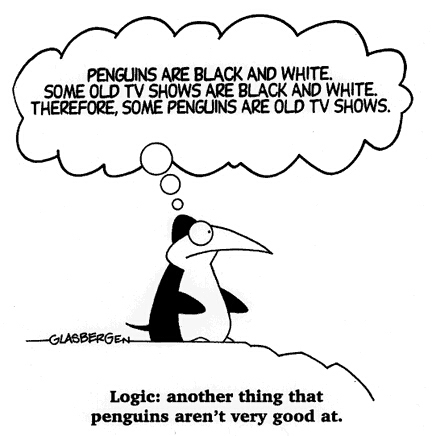
\includegraphics[scale=0.5]{penguin-logic}
  \caption{\label{penguin-logic}Ein Beispiel für einen (ungültigen)
  Syllogismus (Randy Glasbergen, verwendet ohne Erlaubnis).}
\end{figure}


\subsection{Ableitungen}

\begin{defn}Seien~$\varphi$ und~$\psi$ Aussagen in einem Kontext~$\vec x : \vec
A$. Genau dann ist~$\psi$ aus der Voraussetzung~$\varphi$ \emph{ableitbar}, in
Symbolen
$\varphi \seq{\vec x} \psi$,
wenn es eine entsprechende endliche \emph{Ableitung} gibt, welche nur die
in Tafel~\ref{ableitungsregeln:int} aufgeführten Ableitungsregeln verwendet.
\end{defn}

Aus dem Kontext muss hervorgehen, ob man eine Sequenz nur als solche
diskutieren möchte oder ob man ihre Ableitbarkeit unterstellt. Außerdem muss
man sich an die Notation der Ableitungsregeln gewöhnen, drei Beispiele seien im
Folgenden genauer erklärt.

\begin{table}
  \small
  \centering
  \textbf{Strukturelle Regeln} \\
  \vspace{-0.5em}
  \phantom{a}\hfill
  \AxiomC{$\phantom{\seq{\vec x}}$}\UnaryInfC{$\varphi \seq{\vec x} \varphi$}\DisplayProof\hfill
  \AxiomC{$\varphi \seq{\vec x} \psi$}\UnaryInfC{$\varphi[\vec s/\vec x]
  \seq{\vec y} \psi[\vec s/\vec x]$}\DisplayProof\hfill
  \AxiomC{$\varphi \seq{\vec x} \psi$}\AxiomC{$\psi \seq{\vec x}
  \chi$}\BinaryInfC{$\varphi \seq{\vec x} \chi$}\DisplayProof
  \phantom{a}\hfill
  \vspace{2.0em}

  \textbf{Regeln für Konjunktion} \\
  \vspace{-0.5em}
  \phantom{a}\hfill
  \AxiomC{$\phantom{\seq{\vec x}}$}\UnaryInfC{$\varphi \seq{\vec x} \top$}\DisplayProof\hfill
  \AxiomC{$\phantom{\seq{\vec x}}$}\UnaryInfC{$\varphi \wedge \psi \seq{\vec x} \varphi$}\DisplayProof\hfill
  \AxiomC{$\phantom{\seq{\vec x}}$}\UnaryInfC{$\varphi \wedge \psi \seq{\vec x} \psi$}\DisplayProof\hfill
  \AxiomC{$\varphi \seq{\vec x} \psi$}\AxiomC{$\varphi \seq{\vec x} \chi$}\BinaryInfC{$\varphi \seq{\vec x} \psi \wedge \chi$}\DisplayProof
  \phantom{a}\hfill
  \vspace{2em}

  \textbf{Regeln für Disjunktion} \\
  \vspace{-0.5em}
  \phantom{a}\hfill
  \AxiomC{$\phantom{\seq{\vec x}}$}\UnaryInfC{$\bot \seq{\vec x} \varphi$}\DisplayProof\hfill
  \AxiomC{$\phantom{\seq{\vec x}}$}\UnaryInfC{$\varphi \seq{\vec x} \varphi \vee \psi$}\DisplayProof\hfill
  \AxiomC{$\phantom{\seq{\vec x}}$}\UnaryInfC{$\psi \seq{\vec x} \varphi \vee \psi$}\DisplayProof\hfill
  \AxiomC{$\varphi \seq{\vec x} \chi$}\AxiomC{$\psi \seq{\vec x} \chi$}\BinaryInfC{$\varphi \vee \psi \seq{\vec x} \chi$}\DisplayProof
  \phantom{a}\hfill
  \vspace{2em}

  \textbf{Doppelregel für Implikation} \\
  \vspace{-0.5em}
  \phantom{a}\hfill
  \Axiom$\varphi \wedge \psi\ \fCenter\seq{\vec x} \chi$
  \doubleLine
  \UnaryInf$\varphi\ \fCenter\seq{\vec x} \psi \Rightarrow \chi$
  \DisplayProof
  \phantom{a}\hfill
  \vspace{2em}

  \textbf{Doppelregeln für Quantifikation} \\
  \vspace{-0.5em}
  \phantom{a}\hfill
  \Axiom$\varphi\ \fCenter\seq{\vec x, y} \psi$
  \doubleLine
  \UnaryInf$\exists y\?Y\_\! \varphi\ \fCenter\seq{\vec x} \psi$
  \DisplayProof
  {\tiny ($y$ keine Variable von~$\psi$)}
  \hfill
  \Axiom$\varphi\ \fCenter\seq{\vec x, y} \psi$
  \doubleLine
  \UnaryInf$\varphi\ \fCenter\seq{\vec x\phantom{, y}} \forall y\?Y\_\! \psi$
  \DisplayProof
  {\tiny ($y$ keine Variable von~$\varphi$)}
  \hfill\phantom{a}

  \caption{\label{ableitungsregeln:int}Die Schlussregeln intuitionistischer Logik.}
\end{table}

\begin{table}
  \small
  \centering
  \textbf{Regeln für Gleichheit} \\
  \vspace{-0.5em}
  \phantom{a}\hfill
  \AxiomC{$\phantom{\seq{\vec x}}$}
  \UnaryInfC{$\top \seq{x} x = x$}
  \DisplayProof
  \hfill
  \AxiomC{$\phantom{\seq{\vec x}}$}
  \UnaryInfC{$(\vec x = \vec y) \wedge \varphi \seq{\vec z} \varphi[\vec y/\vec x]$}
  \DisplayProof
  \hfill\phantom{a} \\[0.5em]
  (Dabei steht "`$\vec x = \vec y\,$"' für~$x_1 = y_1 \wedge \cdots \wedge x_n =
  y_n$.)
  \vspace{2em}

  \textbf{Prinzip vom ausgeschlossenen Dritten} \\
  \vspace{-0.5em}
  \phantom{a}\hfill
  \AxiomC{$\phantom{\seq{\vec x}}$}
  \UnaryInfC{$\top \seq{\vec x} \varphi \vee \neg\varphi$}
  \DisplayProof
  \hfill\phantom{a}

  \caption{\label{ableitungsregeln:weitere}Weitere Schlussregeln mancher
  formaler Systeme.}
\end{table}


\subsubsection*{Die Schnittregel}

Oberhalb des horizontalen Strichs in der sog. \emph{Schnittregel}
\begin{prooftree}
  \AxiomC{$\varphi \seq{\vec x} \psi$}
  \AxiomC{$\psi \seq{\vec x} \chi$}
  \BinaryInfC{$\varphi \seq{\vec x} \chi$}
\end{prooftree}
sind, nur durch horizontalen Freiraum getrennt, die Voraussetzungen der Regel
aufgeführt. Unterhalb des Strichs steht dann das Urteil, das man aus diesen
Voraussetzungen ziehen darf. Die Schnittregel besagt also: Ist in einem
Kontext~$\vec x$ aus~$\varphi$ die Aussage~$\psi$ ableitbar, und ist ferner
aus~$\psi$ die Aussage~$\chi$ ableitbar, so ist auch aus~$\varphi$
direkt~$\chi$ ableitbar. Die Schnittregel rechtfertigt also die Modularisierung
mathematischer Argumente in Lemmata.


\subsubsection*{Eine der Disjunktionsregeln}

Die Disjunktionsregel
\begin{prooftree}
  \AxiomC{$\varphi \seq{\vec x} \chi$}
  \AxiomC{$\psi \seq{\vec x} \chi$}
  \BinaryInfC{$\varphi \vee \psi \seq{\vec x} \chi$}
\end{prooftree}
besagt, dass, wenn aus~$\varphi$ die Aussage~$\chi$ ableitbar ist, und wenn
ferner auch aus~$\psi$ die Aussage~$\chi$ ableitbar ist, dass dann auch
aus~$\varphi \vee \psi$ die Aussage~$\chi$ ableitbar ist. Diese Regel
rechtfertigt also, bei einer Disjunktion als Voraussetzung einen Beweis durch
Unterscheidung der beiden möglichen Fälle zu führen.


\subsubsection*{Die Doppelregel für den Allquantor}

Der Doppelstrich in der Regel
\begin{prooftree}
  \Axiom$\varphi\ \fCenter\seq{\vec x, y} \psi$
  \doubleLine
  \UnaryInf$\varphi\ \fCenter\seq{\vec x\phantom{, y}} \forall y\?Y\_\! \psi$
\end{prooftree}
für den Allquantor, die nur angewendet werden darf, wenn~$y$ keine freie
Variable in~$\varphi$ ist, deutet an, dass die Regel sowohl wie üblich von oben
nach unten, als auch von unten nach oben gelesen werden kann. Sie besagt, dass
die beiden Urteile
\begin{itemize}
\item "`Im Kontext~$\vec x : \vec A, y : Y$ ist aus~$\varphi$ die
Aussage~$\psi$ ableitbar."'
\item "`Im Kontext~$\vec x : \vec A$ ist aus~$\varphi$ die Allaussage~$\forall
y\?Y{:}\, \psi$ ableitbar."'
\end{itemize}
äquivalent sind. Sie rechtfertigt daher das bekannte Standardvorgehen, um
Allaussagen nachzuweisen: Man nimmt sich ein "`beliebiges, aber festes"'~$y :
Y$, von dem man außer der Zugehörigkeit zu~$Y$ keine weiteren Eigenschaften
unterstellt, und weist die Behauptung dann für \emph{dieses}~$y$ nach.

\begin{aufg}Wieso sind die Variablenbeschränkungen in den Regeln für den
Existenz- und Allquantor nötig?\end{aufg}


\subsubsection*{Umfang der Ableitungsregeln}

\begin{motto}\label{allesformalisierbar}\emph{Alle} Beweise gewöhnlicher Mathematik, die man
gemeinhin als "`vollständig und präzise ausformuliert"' bezeichnet, lassen sich als
Ableitungen im Sinne der Definition formalisieren (ggf. unter Hinzunahme
klassischer logischer Axiome, Mengentheorieaxiome oder Typtheorieaxiome).
\end{motto}

\begin{aufg}Überzeuge dich von dieser Behauptung. \emph{Tipp:} Formalisiere so
viele Beweise deiner Wahl, bis du keine Lust mehr hast.\end{aufg}

Wer nicht so viel Zeit hat, dem sei verraten, dass
Tafel~\ref{ableitungsregeln:int} kein Haufen ungeordneter Ableitungsregeln ist.
Stattdessen sind die Axiome nach den sie betreffenden Junktoren bzw. Quantoren
gruppiert: Sie legen für jedes sprachliche Konstrukt ist fest, wie man es
\emph{einführt} (etwa: "`kann man sowohl~$\varphi$ als auch~$\psi$
ableiten, so auch~$\varphi \wedge \psi$"')
und \emph{eliminiert} (etwa: "`aus~$\varphi \wedge \psi$ folgt
schlicht~$\varphi$"').

\begin{bem}Neben den strukturellen Regeln sticht einzig das Prinzip vom
ausgeschlossenen Dritten aus diesem System von Einführungs- und
Eliminationsprinzipien heraus. Das ist ein rein formal-ästhetisches Argument
gegen klassische Logik.\end{bem}

\begin{bsp}Dass in jedem Kontext die Sequenz~$\varphi \wedge \psi \seq{\vec x}
\psi \wedge \varphi$ ableitbar ist, zeigt folgende Ableitung:
\vspace{-0.5em}
\begin{prooftree}
  \AxiomC{$\varphi \wedge \psi \seq{\vec x} \psi$}
  \AxiomC{$\varphi \wedge \psi \seq{\vec x} \varphi$}
  \BinaryInfC{$\varphi \wedge \psi \seq{\vec x} \psi \wedge \varphi$}
\end{prooftree}
Die beiden Sequenzen oberhalb des Strichs sind Instanzen des
Eliminationsprinzips für die Konjunktion, die Begründung für den Schritt von
oben nach unten ist das Einführungsprinzip.\end{bsp}

\begin{bsp}Folgende Ableitung zeigt, dass~$\top \seq{\vec x} (\varphi
\Rightarrow \varphi)$ ableitbar ist:
\vspace{-0.5em}
\begin{prooftree}
  \AxiomC{$\top \wedge \varphi \seq{\vec x} \varphi$}
  \UnaryInfC{$\top \seq{\vec x} (\varphi \Rightarrow \varphi)$}
\end{prooftree}
Hierbei wurde das Eliminationsprinzip für die Konjunktion und die Doppelregel
für die Implikation angewendet.\end{bsp}

\begin{bsp}Hier ein längeres Beispiel für eine Ableitung (ein Scan
aus~\cite[Seite~832]{johnstone:elephant}):
\begin{center}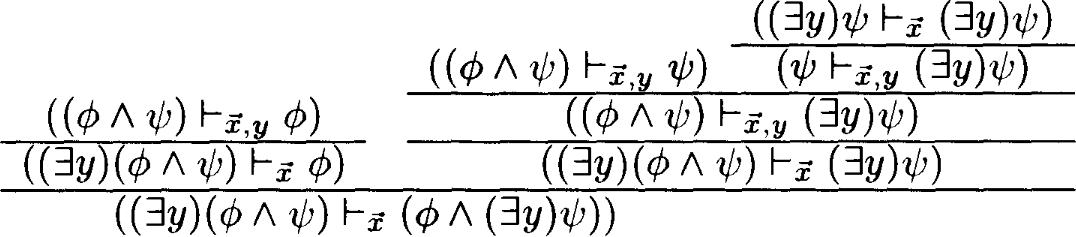
\includegraphics[scale=0.3]{prooftree-elephant.png}\end{center}
Diese Ableitung beweist (eine Richtung des) \emph{Frobenius-Prinzips}. Dabei
kommt die Variable~$y$ nicht in~$\phi$ vor.
\end{bsp}

Nicht verschwiegen werden sollte folgende Ergänzung des formalistischen Kredos:
\begin{motto}Das optimistische Motto~\ref{allesformalisierbar} stimmt nur in
erster Näherung. Es gibt mathematische Gedanken, die nicht formalisierbar
sind.\end{motto}

Zu solchen Gedanken gehören etwa die Überzeugung, jede Art finitistischer
Über\-le\-gung könne in Peano-Arithmetik formalisiert werden; die
Church-Turing-These, der zufolge jede "`algorithmisch berechenbare"' Funktion~$\NN
\to \NN$ durch eine Turing-Maschine gegeben
werden~\cite{plato:ct,goldin:wegner:myth,church70} könne; und manche allgemeinen
mathematischen Prinzipien. Außerdem ist seit Gödel allgemein bekannt, dass es
Beispiele für Aussagen gibt, die zwar in einem formalen System formalisierbar und
von einem höheren Standpunkt aus betrachtet wahr sind (gewissermaßen also einen
informalen Beweis besitzen), im gegebenen System aber nicht bewiesen werden
können.


\subsubsection*{Einschub: Der Quantor für eindeutige Existenz}

Der Quantor~$\exists!$ für eindeutige Existenz kommt in den Ableitungsregeln aus
Tafeln~\ref{ableitungsregeln:int} und~\ref{ableitungsregeln:weitere} nicht vor.
Das ist nicht weiter schlimm, da man diesen durch die anderen sprachlichen
Mittel ausdrücken kann: Die Aussage~"`$\exists!y\?Y\_ \varphi$"' steht für
\[ \exists y\?Y\_ \varphi \quad\wedge\quad
  \forall y\?Y\_ \forall y'\?Y\_
  \varphi \wedge \varphi[y'/y] \Rightarrow y = y'. \]

\begin{aufg}Zeige, dass diese Formalisierung äquivalent ist zur ebenfalls
naheliegenden Umschreibung
\[ \exists y\?Y\_ \bigl(\varphi \wedge (\forall y'\?Y\_ \varphi[y'/y] \Rightarrow y =
y')\bigr). \]
\end{aufg}


\subsection{Peano-Arithmetik und Heyting-Arithmetik}

\begin{defn}Das formale System \emph{Heyting-Arithmetik} ist gegeben durch
\begin{itemize}
\item intuitionistische Logik,
\item die Gleichheitsregeln (siehe Tafel~\ref{ableitungsregeln:weitere}),
\item einem einzigen Typ~$\NN$,
\item einer Termkonstante~$0 : \NN$,
\item einem 1-adischen Termkonstruktor~$S$ (für successor): Ist~$n : \NN$ ein
Term vom Typ~$\NN$, so ist~$S(n) : \NN$ ebenfalls ein Term vom Typ~$\NN$,
\item die Axiome \\
\vspace{-0.5em}
\phantom{a}\hfill
\AxiomC{$\phantom{\seq{\vec x}}$}
\UnaryInfC{$S(n) = 0 \seq{n} \bot$}
\DisplayProof
\hfill
\AxiomC{$\phantom{\seq{\vec x}}$}
\UnaryInfC{$S(n) = S(m) \seq{n,m} n = m$}
\DisplayProof
\hfill
\phantom{a} \\

und das Induktionsprinzip

\vspace{-1.0em}
\phantom{a}\hfill
\AxiomC{$\varphi \seq{\vec x} \psi[0/m]$}
\AxiomC{$\varphi \seq{\vec x, m} \psi \Rightarrow \psi[S(m)/m]$}
\BinaryInfC{$\varphi \seq{\vec x} \forall m\?\NN{:}\ \psi$}
\DisplayProof
\hfill\phantom{a}

\item sowie Regeln für alle primitiv-rekursiven Funktionen, insbesondere also
die erwarteten Regeln für Addition und Multiplikation.
\end{itemize}
\end{defn}

\begin{defn}Das formale System \emph{Peano-Arithmetik} ist genau wie
Heyting-Arithmetik gegeben, nur mit klassischer statt intuitionistischer
Logik.\end{defn}

\begin{defn}Ein formales System heißt genau dann \emph{inkonsistent}, wenn es in
ihm eine Ableitung der Sequenz~$\top \seq{} \bot$ (im leeren Kontext) gibt. Andernfalls heißt es
\emph{konsistent}.\end{defn}


\section{Beziehung zu klassischer Logik}

Auf den ersten Blick scheint intuitionistische Logik schlichtweg weniger
mächtig als klassische Logik zu sein: Viele Aussagen sind klassisch, aber nicht
intuitionistisch ableitbar. Das ist aber nur die halbe
Wahrheit: Es gibt nämlich die \emph{Doppel\-ne\-ga\-tions\-über\-set\-zung},
die Aussagen derart umformt, dass die
Übersetzung genau dann konstruktiv gilt, wenn die ursprüngliche Aussage
klassisch gilt. In diesem Sinn lässt sich also klassische Logik in
intuitionistische einbetten -- man hat also klassische Logik zur Verfügung,
wenn man sie ausnahmsweise verwenden möchte.

Eine Übersetzung in die andere Richtung gibt es leider nicht, man muss größeren
Aufwand treiben, um in einem klassischen Kontext die Sichtweise konstruktiver
Mathematiker zu verstehen. Darauf gehen wir am Ende dieses Abschnitts ein.


\subsection{Die Doppelnegationsübersetzung}

\begin{defn}Die \emph{Doppelnegationsübersetzung} (nach Kolmogorov, Gentzen,
Gödel und anderen) wird rekursiv wie folgt definiert:
\newcommand{\optnegneg}{\textcolor{grey}{\neg\neg}}
\begin{align*}
  \varphi^\circ &:\equiv \neg\neg \varphi \text{ für atomare Aussagen~$\varphi$} \\
  \top^\circ &:\equiv \top \\
  \bot^\circ &:\equiv \bot \\
  (\varphi \wedge \psi)^\circ &:\equiv \optnegneg(\varphi^\circ \wedge \psi^\circ) \\
  (\varphi \vee \psi)^\circ &:\equiv \neg\neg(\varphi^\circ \vee \psi^\circ) \\
  (\varphi \Rightarrow \psi)^\circ &:\equiv \optnegneg(\varphi^\circ \Rightarrow \psi^\circ) \\
  (\forall x\?X{:}\ \varphi)^\circ &:\equiv \optnegneg\forall x\?X{:}\ \varphi^\circ \\
  (\exists x\?X{:}\ \varphi)^\circ &:\equiv \neg\neg\exists x\?X{:}\ \varphi^\circ
\end{align*}
\end{defn}

\begin{bem}Da~$\neg\varphi :\equiv (\varphi \Rightarrow \bot)$,
gilt~$(\neg\varphi)^\circ \equiv \neg(\varphi^\circ)$.\end{bem}

\begin{aufg}Beweise durch Induktion über den Aussageaufbau, dass man auf die grau
gesetzten Doppelnegationen verzichten kann. Gewissermaßen besteht also der
einzige Unterschied zwischen klassischer und intuitionistischer Logik in der
Interpretation der Disjunktion und der Existenzquantifikation: Diese sagen
konstruktiv mehr aus als in klassischer Logik.\end{aufg}

\begin{satz}\label{dnt:proof}Seien~$\varphi$, $\psi$ beliebige Aussagen in einem Kontext~$\vec x$.
\begin{enumerate}
\item Klassisch gilt: $\varphi^\circ \Longleftrightarrow \varphi$.
\item Intuitionistisch gilt: $\neg\neg\varphi^\circ \Longrightarrow
\varphi^\circ$.
\item Wenn~$\varphi \seq{\vec x} \psi$ klassisch, dann~$\varphi^\circ \seq{\vec
x} \psi^\circ$ intuitionistisch; und umgekehrt.
\end{enumerate}
\end{satz}
\begin{proof}
\begin{enumerate}
\item Klar, für jede Aussage~$\chi$ ist~$\neg\neg\chi \Leftrightarrow \chi$
eine klassische Tautologie.
\item Induktion über den Aussageaufbau, ausgelassen.
\item Die Rückrichtung ist wegen der Ab\-wärts\-kom\-pa\-ti\-bi\-li\-tät
intuitionistischer Logik und Teilaussage~a) trivial.

Für die Hinrichtung müssen wir in einer Induktion über den Aufbau klassischer Ableitungen
nachweisen, dass wir jeden logischen Schluss klassischer Logik in der
Doppelnegationsübersetzung intuitionistisch nachvollziehen können. (Aus diesem
Grund mussten wir im vorherigen Abschnitt formal definieren, was wir unter
Ableitungen verstehen wollen.)

Etwa müssen wir zeigen, dass die übersetzte Schnittregel gültig ist:
\begin{prooftree}
  \AxiomC{$\varphi^\circ \seq{\vec x} \psi^\circ$}
  \AxiomC{$\psi^\circ \seq{\vec x} \chi^\circ$}
  \BinaryInfC{$\varphi^\circ \seq{\vec x} \chi^\circ$}
\end{prooftree}
Aber das ist klar, denn das ist wieder eine Instanz der intuitionistisch
zulässigen Schnittregel. Ein interessanteres Beispiel ist die übersetzte Form
von einer der Disjunktionsregeln:
\begin{prooftree}
  \AxiomC{}
  \UnaryInfC{$\varphi^\circ \seq{\vec x} \neg\neg(\varphi^\circ \vee \psi^\circ)$}
\end{prooftree}
Die Gültigkeit dieser Regel folgt aus der Disjunktionsregel und der
intuitionistischen Tautologie~$\chi \Rightarrow \neg\neg\chi$. Als letztes
und wichtigstes Beispiel wollen wir die Übersetzung des klassischen Axioms vom
ausgeschlossenen Dritten diskutieren:
\begin{prooftree}
  \AxiomC{}
  \UnaryInfC{$\top \seq{\vec x} \neg\neg(\varphi^\circ \vee \neg\varphi^\circ)$}
\end{prooftree}
Dass diese Regel intuitionistisch zulässig ist, haben wir in Übungsblatt~1
gesehen. Die Untersuchung aller weiteren Schlussregeln überlassen wir den Leser
(Übungsblatt~2).\qedhere
\end{enumerate}
\end{proof}

\begin{kor}Zeigt Peano-Arithmetik einen Widerspruch, so auch
Heyting-Arithmetik.\end{kor}
\begin{proof}Man kann leicht nachprüfen, dass die
Doppelnegationsübersetzungen der Peano-Axiome wiederum Instanzen den
Peano-Axiome sind und daher auch in Heyting"=Arithmetik gelten. Daher kann man
eine Ableitung von~$\bot$ in Peano-Arithmetik in eine Ableitung
von~$\bot^\circ \equiv \bot$ in Heyting-Arithmetik überführen.\end{proof}

Folgendes Lemma werden wir erst später, in Abschnitt~\ref{sect:friedman} über
Friedmans Trick, benötigen:
\begin{lemma}\label{dnt:geom}Sei~$\varphi$ eine Aussage, in der nur~$\top$, $\bot$,
$\wedge$, $\vee$ und $\exists$ (über
bewohnte Typen), aber nicht~$\Rightarrow$ und~$\forall$ vorkommen. Dann gilt
intuitionistisch: $\varphi^\circ \Longleftrightarrow \neg\neg\varphi$.
\end{lemma}
\begin{proof}Induktion über den Aussageaufbau.\end{proof}


\subsection{Interpretation der übersetzten Aussagen}

Die konstruktive Bedeutung übersetzter Aussagen lässt sich wegen der Vielzahl
vorkommender nichttrivialer doppelter Verneinungen nicht sofort überblicken. Es
gibt aber eine aus der theoretischen Informatik stammende
\emph{Zeitsprungmetapher}, mit der man den Inhalt übersetzter Aussagen doch
verstehen kann.

Dazu erinnern wir zunächst an die Dialogmetapher zur Interpretation logischer
Aussagen:
Wir stellen uns ein besonders kritisches Gegenüber vor, das unsere Behauptung
bezweifelt. In einem Dialog versuchen wir dann, das Gegenüber zu überzeugen.
Eine typische Stetigkeitsüberzeugung sieht etwa wie folgt aus:

\begin{dialogue}
\Eve Ich gebe dir~$x = \cdots$ und~$\varepsilon = \cdots$ vor.
\Alice Gut, dann setze ich~$\delta = \cdots$.
\Eve Dann ist hier ein~$\tilde x = \cdots$ zusammen mit einem Beleg von~$|x -
\tilde x| < \delta$.
\Alice Dann gilt tatsächlich~$|f(x) - f(\tilde x)| < \varepsilon$,
wie von mir behauptet, denn \ldots
\end{dialogue}

In Tafel~\ref{bhk} (Seite~\pageref{bhk}) ist festgelegt, nach welchen
Spielregeln Alice und Eve bei solchen Dialogen miteinander kommunizieren
müssen. Exemplarisch seien einige nochmal betont:
\begin{itemize}
\item Wenn Eve von Alice einen Beleg von~$\varphi \vee \psi$ fordert,
muss Alice einen Beleg von~$\varphi$ oder einen Beleg von~$\psi$ präsentieren.
Sie darf sich nicht mit einem "`angenommen, keines von beiden gälte"'
herausreden.
\item Wenn Eve von Alice einen Beleg von~$\varphi \Rightarrow \psi$
fordert, muss Alice ihr versprechen, Belege von~$\varphi$ in Belege von~$\psi$
überführen zu können. Dieses Versprechen kann Eve herausfordern, indem sie
einen Beleg von~$\varphi$ präsentiert; Alice muss dann in der Lage sein, mit
einem Beleg von~$\psi$ zu antworten.
\item Für die Negation als Spezialfall der Implikation gilt folgende Spielregel: Wenn Eve von
Alice einen Beleg von~$\neg\varphi \equiv (\varphi \Rightarrow \bot)$ verlangt,
muss Alice in der Lage sein, aus einem präsentierten Beleg von~$\varphi$ einen
Beleg von~$\bot$ zu produzieren. Wenn das betrachtete formale System konsistent
ist, gibt es keinen solchen Beleg; Alice kann unter der Konsistenzannahme also
nur dann~$\neg\varphi$ vertreten, wenn es keinen Beleg von~$\varphi$ gibt.
\end{itemize}

Als Motto können wir festhalten:

\begin{motto}
Eine Aussage~$\varphi$ intuitionistisch zu behaupten, bedeutet, in jedem
Dialog~$\varphi$ belegen zu können.
\end{motto}

Dank der Doppelnegationsübersetzung können wir damit auch eine
Dialoginterpretation klassischer Behauptungen angeben. Es stellt sich heraus,
dass die folgende Metapher sehr tragfähig ist. Diese wollen wir dann erst an
einem Beispiel veranschaulichen bevor wie sie begründen.

\begin{motto}
Eine Aussage~$\varphi$ klassisch zu behaupten (also~$\varphi^\circ$
intuitionistisch zu behaupten), bedeutet, in jedem Dialog~$\varphi$ belegen zu
können, wobei man aber beliebig oft Zeitsprünge in die Vergangenheit
durchführen darf.
\end{motto}


\subsubsection*{Beispiel: das Prinzip vom ausgeschlossenen Dritten}

Wir wollen sehen, wie man das klassische Prinzip~$\varphi \vee
\neg\varphi$ mit Hilfe von Zeitsprüngen vertreten kann.
\begin{dialogue}
\Eve Zeige mir~$\varphi \vee \neg\varphi$!
\Alice Gut! Es gilt~$\neg\varphi$.
\end{dialogue}
Wenn~$\varphi$ eine allgemeine Aussage ist, kann Alice nicht wissen,
ob~$\varphi$ oder~$\neg\varphi$ gilt. Sie hat daher an dieser Stelle geblufft.
Da sie eine Implikation behauptet -- nämlich~$(\varphi \Rightarrow \bot)$ --, ist nun Eve
wieder an der Reihe. Sie kann nur dann in ihrem Vorhaben, Alice zu widerlegen,
fortfahren, wenn sie einen Beleg von~$\varphi$ präsentiert und dann Alice
herausfordert, ihr Versprechen, daraufhin einen Beleg von~$\bot$ zu
präsentieren, einzulösen.

Wenn es keinen Beleg von~$\varphi$ gibt, ist das Streitgespräch daher an dieser
Stelle beendet, und Alice hat sogar die Wahrheit gesagt. Andernfalls geht es
weiter:
\begin{dialogue}
\Eve Aber hier ist ein Beleg von~$\varphi$: $x$. Belege mir nun~$\bot$!
\end{dialogue}
Wenn Alice nicht die Inkonsistenz des untersuchten formalen Systems nachweisen
kann, hat sie nun ein Problem: Ihre Lüge von Beginn straft sich, sie kann das
Gespräch nicht fortsetzen. Sie muss daher in einem Logikwölkchen verschwinden
und in der Zeit zurückspringen:
\begin{dialogue}
\Eve Zeige mir~$\varphi \vee \neg\varphi$!
\Alice Gut! Es gilt~$\varphi$, hier ist ein Beleg: $x$.
\end{dialogue}
Damit ist das Gespräch abgeschlossen.

Wer Zeitsprünge dieser Form betrügerisch findet, hat die
Grund\-über\-zeu\-gung konstruktiver Mathematik bereits verinnerlicht: In diesem (und
nur diesem) Sinn ist klassische Logik tatsächlich betrügerisch. Das macht
klassische Logik aber nicht trivial: Auch mit Zeitsprüngen kann man nicht jede
beliebige Aussage in einem Dialog vertreten. Wenn man etwa obiges Vorgehen
mit der im Allgemeinen ungerechtfertigten Aussage~$\varphi \vee \neg\psi$
versucht, wird man sehen, dass auch die Fähigkeit zu Zeitsprüngen
nicht hilft.


\subsubsection*{Dasselbe Beispiel, konservativer interpretiert}

Um zu sehen, dass die Zeitsprungmetapher berechtigt ist, wollen wir
exemplarisch dasselbe Beispiel erneut untersuchen, diesmal aber ohne die
Metapher. Wir wollen also einen
Dialog zur
Dop\-pel\-ne\-ga\-tions\-über\-set\-zung des Prinzips vom ausgeschlossenen
Dritten, also zu $\neg\neg(\varphi^\circ \vee \neg\varphi^\circ)$, führen. Da wir
für beliebige Aussagen~$\varphi$ sogar das Prinzip $\neg\neg(\varphi \vee
\neg\varphi)$ nachweisen können, ausgeschrieben
\[ ((\varphi \vee \neg\varphi) \Rightarrow \bot) \Rightarrow \bot, \]
und dieses geringfügig übersichtlicher ist, wollen wir tatsächlich dieses in Dialogform
belegen.

\begin{dialogue}
\Eve Zeige mir~$\neg\neg(\varphi \vee \neg\varphi)$!
Präsentiere mir also einen Beleg von~$\bot$, wobei du auf mich zurückkommen
kannst, wenn du einen Beleg von~$\varphi \vee \neg\varphi$ hast; dann
würde ich Beleg von~$\bot$ produzieren.
\Alice Gut! Dann komme ich sofort auf dich zurück, denn ich habe einen Beleg
von~$\neg\varphi$. $(\star)$
\end{dialogue}

Wie oben ist das Gespräch an dieser Stelle beendet, wenn Eve nicht einen Beleg
von~$\varphi$ produzieren kann, mit dem sie Alice herausfordern könnte. Falls
sie das doch schafft, geht es wie folgt weiter:

\begin{dialogue}
\Eve Ach wirklich? Hier ist ein Beleg von~$\varphi$: $x$. Zeige mir nun einen
Beleg von~$\bot$!
\Alice Dann komme ich auf deine Verpflichtung mir gegenüber ein zweites Mal
zurück -- hier ist ein Beleg von~$\varphi \vee \neg\varphi$: $x$.
\Eve Stimmt. Dann ist hier Beleg von~$\bot$: $y$.
\Alice Danke. Dann ist hier ein Beleg von~$\bot$: $y$. Damit habe ich meine
Pflicht erfüllt.
\Eve Stimmt. Dann erfülle ich meinen Teil der Verpflichtung (Stelle~$(\star)$),
hier ist Beleg von~$\bot$: $z$.
\Alice Danke. Dann ist hier Beleg von~$\bot$, wie gefordert: $z$.
\end{dialogue}

% XXX Fazit

% XXX Curry-Howard

Doppelnegationsübersetzung, Continuation-Passing-Style Transformation,
LCM, Stein der Weisen, \ldots

% XXX: Feinere Unterschiede


\subsection{Die umgekehrte Richtung: Modelle für intuitionistische Logik}

Mit der Doppelnegationsübersetzung kann eine konstruktive Mathematikerin auf
eine sehr einfache Art und Weise einen klassischen Kollegen verstehen: Wenn ein
klassischer Mathematiker eine Aussage~$\varphi$ behauptet, muss man als
konstruktiv nur~$\varphi^\circ$ verstehen.

Für die umgekehrte Richtung gibt es keine Übersetzung: Es gibt keine
Aussagentransformation~$\varphi \mapsto \varphi^\#$ mit den Eigenschaften
\begin{enumerate}
\item $\varphi \Longleftrightarrow \varphi^\#$ intuitionistisch und
\item genau dann $\varphi \seq{\vec x} \psi$ intuitionistisch, wenn $\varphi^\#
\seq{\vec x} \psi^\#$ klassisch.
\end{enumerate}
Denn aus der ersten Eigenschaft würde wegen der Abwärtskompatibilität
intuitionistischer Logik zu klassischer Logik ja klassisch die Äquivalenz $\varphi \Leftrightarrow
\varphi^\#$ folgen; das ist mit Eigenschaft~b) unverträglich.

Eine klassische Mathematikerin hat es also schwerer, konstruktiv arbeitende
Kollegen zu verstehen. Sie muss dazu geeignete \emph{Modelle} betrachten.


\subsubsection*{Topologische Modelle für propositionale intuitionistische
Logik}

Mit \emph{propositionaler} Logik bezeichnet man das Fragment, in dem keine
Variablen und daher insbesondere keine Quantoren vorkommen. (Ihre klassische
Variante kann man noch mit Wahrheitstafeln vollständig verstehen.)

Jeder topologischer Raum~$X$ liefert ein Modell~$\Ouv(X)$ für propositionale
intuitionistische Logik: Wenn man jeder atomaren Aussage~$\varphi$ eine
bestimmte offene Menge~$\brak{\varphi} \subseteq X$ zuordnet, kann man die
Interpretation der restlichen Aussagen gemäß folgender Definition festlegen.
\begin{defn}[topologische Interpretation zusammengesetzter Aussagen]
\begin{align*}
  \brak{\top} &:= X \\
  \brak{\bot} &:= \emptyset \\
  \brak{\varphi \wedge \psi} &:= \brak{\varphi} \cap \brak{\psi} \\
  \brak{\varphi \vee \psi} &:= \brak{\varphi} \cup \brak{\psi} \\
  \brak{\varphi \Rightarrow \psi} &:=
    \hcancel{$\brak{\varphi}^c \cup \brak{\psi}$}{0pt}{3pt}{0pt}{-2pt} =
    \interior(\brak{\varphi}^c \cup \brak{\psi})
\end{align*}
\end{defn}
Dabei bezeichnet~$U^c$ das Komplement von~$U$ in~$X$. Die Verwendung
von~$(\brak{\varphi}^c \cup \brak{\psi})$ würde die Menge der offenen Mengen
von~$X$ verlassen und ist daher schon aus diesem formalen Grund keine gute
Idee; Abhilfe schafft das Nehmen des inneren Kerns.

Anschaulich kann man sich~$\brak{\varphi}$ als den Ort, wo~$\varphi$ erfüllt
ist, vorstellen. Wenn~$\brak{\varphi} = \emptyset$ gilt, gilt~$\varphi$ also
nirgendwo; wenn~$\brak{\varphi} = X$ gilt, gilt~$\varphi$ überall; wenn~$X$
nicht gerade nur zwei offene Mengen besitzt, sind aber auch viele weitere
Abstufungen möglich. In diesem Sinn ist~$\Ouv(X)$ ein Modell mit mehr als zwei
Wahrheitswerten.

\begin{bsp}Sei~$X$ die Erdoberfläche. Dann kann man zwei atomare Aussagen~$A$
und~$B$ mit den Interpretationen
\begin{align*}
  \brak{A} &:= \{ x \in X \,|\, \text{an der Stelle~$x$ regnet es} \} \\
  \brak{B} &:= \{ x \in X \,|\, \text{an der Stelle~$x$ hat es mehr
  als~$20$ Grad} \}
\end{align*}
definieren. Die Aussage~$A \wedge B$ hat dann die Interpretation
$\brak{A \wedge B} = \brak{A} \wedge \brak{B}$, beschreibt also den Ort
derjenigen Stellen auf der Erde, an denen es bei mehr als~$20$ Grad
regnet.\end{bsp}

Die folgende Definition zeigt, dass diese Definition die Regeln
intuitionistischen Schließens respektiert und daher sinnvoll ist:
\begin{prop}Wenn~$\varphi \seq{} \psi$ intuitionistisch (im Fragment ohne
Variablen), dann $\brak{\varphi} \subseteq \brak{\psi}$.\end{prop}
\begin{proof}
Wir müssen zeigen, dass die offenen Mengen von~$X$ den Schlussregeln
propositionaler intuitionistischer Logik gehorchen. Etwa lautet die
Interpretation der Schnittregel
\begin{prooftree}
  \AxiomC{$\brak{\varphi} \subseteq \brak{\psi}$}
  \AxiomC{$\brak{\psi} \subseteq \brak{\chi}$}
  \BinaryInfC{$\brak{\varphi} \subseteq \brak{\chi}$}
\end{prooftree}
und ist offensichtlich erfüllt: Wenn~$\brak{\varphi} \subseteq \brak{\psi}$
und~$\brak{\psi} \subseteq \brak{\chi}$, dann auch~$\brak{\varphi} \subseteq
\brak{\chi}$. Die Interpretation einer der Konjunktionsregeln lautet
\vspace{-1em}
\begin{prooftree}
  \AxiomC{$\phantom{\seq{}}$}
  \UnaryInfC{$\brak{\varphi \wedge \psi} \subseteq \brak{\varphi}$}
\end{prooftree}
und ist ebenfalls erfüllt: Denn~$\brak{\varphi \wedge \psi} = \brak{\varphi}
\cap \brak{\psi} \subseteq \brak{\varphi}$. Die restlichen Fälle überlassen wir
dem Leser.\end{proof}

Eine andere Definition als die oben gegebene ist im Übrigen gar nicht möglich,
wenn man möchte, dass diese Proposition gültig bleibt. Schnell kann man das wie
folgt einsehen: Die Schlussregeln beschreiben \emph{universelle Eigenschaften}
für~$\top$, $\bot$, $\wedge$, $\vee$ und~$\Rightarrow$ und legen daher ihre
Interpretationen schon eindeutig fest.

\begin{bem}Wenn man auch in seiner Meta-Logik konstruktiv arbeiten möchte,
sollte man besser
\[ \brak{\varphi \Rightarrow \psi} :=
  \bigcup \{ U \,|\, \text{$U \subseteq X$ offen, $U \cap \brak{\varphi}
  \subseteq \brak{\psi}$} \} \]
definieren. Da in klassischer Logik genau dann~$U \subseteq V^c \cup W$,
wenn~$U \cap V \subseteq W$, ist diese Definition in klassischer Logik zu
obiger äquivalent.\end{bem}

\begin{bem}Die Menge~$\Ouv(X)$ der offenen Teilmengen von~$X$ hat die Struktur
einer \emph{Heyting-Algebra}. Etwas allgemeiner kann man Modelle
intuitionistischer propositionaler Logik in beliebigen Heyting-Algebren
untersuchen (und nicht nur solchen, die von topologischen Räumen
stammen).\end{bem}


\subsubsection*{Topologische Interpretation des Prinzips vom ausgeschlossenen
Dritten}

Die topologische Interpretation von~$\varphi \vee \neg\varphi$ ist die offene
Menge
\[ \brak{\varphi \vee \neg\varphi} = \brak{\varphi} \cup \interior
(\brak{\varphi}^c), \]
also die Vereinigung von~$\brak{\varphi}$ mit dem Inneren ihres Komplements. Es
ist klar, dass diese Vereinigung in den meisten interessanten Fällen nicht
gleich ganz~$X$ ist -- es fehlt der Rand von~$\brak{\varphi}$; das Prinzip vom
ausgeschlossenen Dritten gilt also in den
wenigsten topologischen Modellen.

% XXX: Anschauliche Interpretation


\subsubsection*{Ausblick: Kategorielle Modelle für intuitionistische Prädikatenlogik}

Ein Modell für intuitionistische Prädikatenlogik benötigt nicht nur
Wahrheitswerte, sondern auch Objekte, aus denen die Variablenwerte gezogen
werden können: Grundlage für ein solches Modell ist also eine Kategorie, in der
jeder Typ des untersuchten intuitionistischen Systems durch ein Objekt der
Kategorie repräsentiert wird. Um die Junktoren~$\wedge$, $\vee$
und~$\Rightarrow$ interpretieren zu können, muss für jedes Objekt~$A$ der
Kategorie die Menge der Unterobjekte von~$A$ die Struktur einer Heyting-Algebra
tragen. Den All- und den Existenzquantor interpretiert man als Rechts-
bzw. Linksadjungierte zu induzierten Rückzugsabbildungen.

Wichtige Beispiele für solche Kategorien sind \emph{Topoi}. In
Abschnitt~\ref{sect:topoi} gehen wir genauer darauf ein, wie man in ihnen
intuitionistische Logik interpretiert.
Zur weiterführenden Lektüre eignen sich das
Vorlesungsskript~\cite{streicher:ctcl} und der Artikel~\cite{vickers:loctop}.


\section[Beziehung zur theoretischen Informatik: die
Curry-Howard-Korrespondenz]{Beziehung zur theoretischen Informatik: \newline die
Curry-Howard-Korrespondenz}

% XXX: wadler:curry-howard zitieren

Unter der Curry-Howard-Korrespondenz versteht man grob folgendes fundamentale
Motto, das intuitionistische Logik und theoretische Information in Beziehung
setzt:

\begin{motto}Eine Aussage~$\varphi$ ist genau dann intuitionistisch ableitbar,
wenn es ein Computerprogramm vom Typ~$\varphi$ gibt.\end{motto}

Hierbei wird~$\varphi$ einerseits als Aussage, andererseits als Typ
interpretiert. Beispiele sollen diesen Doppelgebrauch deutlich machen.


\subsection{Beispiele}

\subsubsection*{Beispiel 1}

Konstruktiv gilt offensichtlich~$A \Rightarrow A$. Ein expliziter Beweis
verläuft wie folgt: \emph{Gelte~$A$. Dann gilt~$A$.} Wenn man dem Leser noch
weiter helfen möchte, kann man den zweiten Schritt noch explizit begründen:
\begin{quote}\emph{Gelte~$A$. $(\star)$ \\ Wegen~$(\star)$ gilt dann
auch~$A$.}\end{quote}
Man kann sich auch trauen, den gegebenen Zeugen von~$A$ mit einem
Kleinbuchstaben statt einem Symbol zu bezeichnen. Dann kann man schreiben:
\begin{quote}\emph{Sei~$p\?A$. Dann gilt~$p\?A$.}\end{quote}
Hieraus ist nun folgendes Computerprogramm ableitbar:
\[ \begin{array}{@{}rcl@{}}
  A &\longrightarrow& A \\
  p &\longmapsto& p
\end{array} \]
Dieses Computerprogramm hat den \emph{Typ}~$(A \to A)$. Man beachte, dass
dasselbe Symbol~"`$A$"' hier je nach Kontext als \emph{Aussage} oder als
\emph{Typ} (den man sich in erster Näherung als Menge der Zeugen der
Aussage~$A$ vorstellen kann) verwendet wird.


\subsubsection*{Beispiel 2}

Konstruktiv gilt~$A \Rightarrow (B \Rightarrow A)$. Ein Beweis verläuft
wie folgt:
\begin{quote}\emph{Sei~$p\?A$, dann ist~$(B \Rightarrow A)$ zu zeigen. Sei
dazu~$q\?B$ gegeben, dann ist~$A$ zu zeigen. Das ist klar
wegen~$p\?A$.}\end{quote}
Daraus kann man folgendes Programm ableiten:
\[ \begin{array}{@{}rcl@{}}
  A &\longrightarrow& B^A \\
  p &\longmapsto& (q \mapsto p)
\end{array} \]
Dabei bezeichnet~"`$B^A$"' den Typ der Funktionen von~$A$ nach~$B$.


\subsubsection*{Beispiel 3}

Konstruktiv gilt~$A \wedge B \Rightarrow A$, mit folgendem Beweis:
\begin{quote}\emph{Sei~$p\?(A \wedge B)$. Dann steckt in~$p$ ein Zeuge
von~$A$.}\end{quote}
Das zugehörige Computerprogramm lautet wie folgt:
\[ \begin{array}{@{}rcl@{}}
  A \times B &\longrightarrow& A \\
  (p,q) &\longmapsto& p
\end{array} \]
Hierfür ist der zu~$A \wedge B$ gehörige Typ~$A \times B$.


\subsection{Interpretation}

Die Curry-Howard-Korrespondenz hat einen ganz praktischen Nutzen: Aus
intuitionistischen Beweisen kann man Computerprogramme extrahieren und
umgekehrt. Beide Richtungen sind interessant: Etwa kann man offensichtlich ein
Computerprogramm schreiben, das zu einer Eingabe~$n \? \NN$ eine Primzahl~$p
\geq n$ produziert. Daher ist auch die entsprechende Aussage intuitionistisch
ableitbar:~$\forall n{:}\NN{:}\ \exists p \geq n{:}\ \text{$p$ prim}$.

Die Umkehrung ist im Kontext formaler Methoden in der Informatik wichtig.


\subsection{Genauere Formulierung}

Eine genauere Formulierung ist folgende: Es gibt eine 1:1--Korrespondenz
zwischen \emph{Ableitungen} einer Aussage~$\varphi$ einerseits und
\emph{Termen} vom Typ~$\varphi$ andererseits. Für eine völlig präzise
Formulierung muss man nur noch das gewählte Ableitungssystem und den gewählten
Termkalkül sowie die
Übersetzung von Aussagen zu Typen festlegen. Als Termkalkül kann man etwa den
einfach getypten~$\lambda$-Kalkül verwenden.

Als Korollar folgt aus der präziseren Formulierung das oben angegebene Motto:
Genau dann gibt es eine Ableitung, wenn es einen entsprechenden Term gibt.

Der Beweis ist übrigens trivial, wenn man die Behauptung nur präzise genug
formuliert hat. Denn die Ableitungsregeln entsprechen~1:1 den
Termkonstruktionsregeln.

Für Details sei der Übersichtsartikel~\cite{wadler:curry-howard} von Philip
Wadler (einem der Väter der Pro\-gram\-mier\-spra\-che Haskell) empfohlen. Wer die
Curry-Howard-Korrespondenz wirklich verstehen möchte, kann das
Vorlesungsskript~\cite{sorensen:urzyczyn:curryhoward} zurate ziehen. Es enthält
auch eine Einführung in den~$\lambda$-Kalkül.


\section{Hilberts Programm}

\subsection[Die mathematische Welt um 1900]{Die mathematische Welt um 1900
\qquad\small[unvollständig und fehlerhaft]}

Man erzählt sich folgende Geschichte. Im letzten Viertel des 19.~Jahrhunderts
kamen in der Mathematik neue, abstrakte Methoden auf. Dazu gehörte vor allem
Cantors Mengenlehre, die mit ihrer Akzeptanz des \emph{aktual Unendlichen} ein
Tabu brach: Es war zwar jeder mit dem Konzept \emph{potenzieller} Unendlichkeit
vertraut, wie etwa der Vorstellung, dass die natürlichen Zahlen "`nie
aufhören"', dass man "`immer weiter zählen kann"'. Aber manche hatten Angst
davor, unendlich viele Objekte zu einer vollendeten Menge zusammenzufassen.

Insbesondere wurde die Verwendung des Prinzips
\[ \neg\forall x\?X{:}\, \neg\varphi(x) \quad\Longrightarrow\quad
  \exists x\?X{:}\, \varphi(x) \]
kritisiert. Dies erscheint von unserem heutigen Standpunkt verwunderlich: Denn
dieses Prinzip folgt ja sofort aus dem Prinzip vom ausgeschlossenen Dritten,
welches man stets als evident annahm. Man muss aber zwischen verschieden
mächtigen Instanzen des Prinzips unterscheiden. Etwa ist für natürliche
Zahlen~$n$ die Aussage
\[ n = 0 \quad\vee\quad n \neq 0 \]
völlig unkritisch, sie ist sogar konstruktiv beweisbar. Die analoge Aussage für
reelle Zahlen~$x$ ist zwar nicht konstruktiv haltbar, aber im 19.~Jahrhundert
war noch nicht der Rahmen gegeben, um das einzusehen bzw. überhaupt die Frage
nach formaler konstruktiver Ableitbarkeit zu stellen. Stattdessen wurde diese
Aussage ebenfalls als einleuchtend empfunden und akzeptiert.

Widerspruchsbeweise wurden also durchaus akzeptiert. (Die manchmal behauptete
Aussage, klassische Logik sei erst im 20.~Jahrhundert aufgekommen, ist also
nicht richtig.) Angst bestand nur vor Anwendungen des Prinzips vom
ausgeschlossenen Dritten in Kombination mit unendlich großen Mengen. So
zerfielen die Mathematiker in zwei Lager: Solche, die neue abstrakte Methoden
mit Begeisterung aufnahmen, und solche, die den neuen Entwicklungen kritisch
gegenüber standen.

David Hilbert gehörte zu den Fans, nicht zuletzt deswegen, weil er selbst mit
nichtkonstruktiven Methoden seinen \emph{Basissatz} bewies, mit dem er
international bekannt wurde: Dieser besagt, dass jedes Ideal des
Polynomrings~$k[X_1,\ldots,X_n]$ endlich erzeugt ist. Vor Hilberts Beweis war
das überhaupt nicht klar, und es gab eine große Industrie, um explizit Erzeuger in
konkreten Fällen zu bestimmen. Da Hilbert kein Verfahren angeben konnte,
um die Erzeuger zu berechnen, sondern lediglich zeigte, dass die Annahme,
es gäbe kein endliches Erzeugendensystem, zu einem Widerspruch führte, vertrat
etwa Paul Gordan, der \emph{König der
Invariantentheorie}, folgende Meinung über Hilberts Resultat:
\begin{quote}
\emph{Das ist nicht Mathematik, das ist Theologie.}
\end{quote}

Um seine Kritiker zufrieden zu stellen, wollte Hilbert daher zeigen, dass man
die neuen abstrakten Methoden \emph{eliminieren} konnte. Damit hat er nicht die
Abschaffung derselbigen gemeint -- im Gegenteil: Er wollte ihre Zulässigkeit
rechtfertigen, indem er zeigen wollte, dass man aus jedem Beweis einer
konkreten Aussage, der abstrakte Methoden verwendet, einen Beweis erhalten
kann, der nur finitistisch zulässige Schlussweisen verwendet.

\begin{aufg}[Hilberts Programm]Zeige, dass man aus jedem Beweis einer konkreten
Aussage, welcher beliebige ideelle Prinzipien (etwa das Prinzip vom ausgeschlossenen
Dritten für beliebige Aussagen, das Auswahlaxiom oder maximale Ideale in der Algebra)
verwendet, einen finitistisch zulässigen Beweis erhalten kann.\end{aufg}

Dabei ist eine \emph{konkrete Aussage} eine solche, in deren Formulierung nur
die natürlichen Zahlen, aber keine höheren Konzepte wie Mengen natürlicher
Zahlen oder gar Mengen von Mengen vorkommen. Diese Beschränkung in Hilberts
Programm ist sicherlich notwendig: Etwa kann man offensichtlich keine Aussage
über Mengen ohne Verwendung von Mengen zu beweisen.

\begin{bsp}Die Aussage, dass die Menge der Primzahlen nicht endlich ist, ist
nicht konkret. Äquivalent ist aber die Aussage, dass zu jeder vorgegebenen
Schranke eine Primzahl existiert, die größer als die Schranke ist; und diese
ist konkret.\end{bsp}

In voller Allgemeinheit gilt Hilberts Programm seit 1931 als
\emph{gescheitert}. Denn in diesem Jahr veröffentlichte Gödel sein
Unvollständigkeitsresultat: Die Aussage \emph{Peano-Arithmetik ist konsistent}
lässt sich als "`konkrete Aussage"' formulieren und leicht mit abstrakten
Methoden beweisen (in üblicher Mengenlehre liefert die unendliche Menge~$\NN$
ein Modell), kann aber keinen finitistisch zulässigen Beweis besitzen, da es
nach Gödels Unvollständigkeitssatz nicht einmal einen Beweis in der stärkeren
Peano-Arithmetik geben kann.

Teilweise kann Hilberts Programm jedoch schon realisiert werden, unter anderem
in Analysis und Algebra: Mittels \emph{proof mining} kann aus klassischen
Beweisen mehr oder weniger systematisch noch konstruktiver Inhalt extrahiert
werden. Je nach Situation kann \emph{konstruktiver Inhalt} etwa
explizite Schranken für Konstanten,
stetige (oder noch bessere) Abhängigkeit von Parametern,
explizite Zeugen von Existenzbehauptungen oder
Algorithmen
umfassen.

\begin{motto}\label{motto:inhaltvonbeweisen}In einem \emph{Beweis} einer
Aussage steckt viel mehr Inhalt als die bloße Information, dass die Aussage
wahr ist.\end{motto}

Dieses Motto ist keine tiefe Einsicht: \emph{Natürlich} steckt in
einem Beweis einer Aussage viel mehr Inhalt als in einer bloßen
Wahrheitsbekundung -- nämlich ein \emph{Grund}, wieso die Aussage stimmt.
Interessant ist, dass man dieses Motto auch formal ernst nehmen kann.

Siehe~\cite{plato:hilbert,zach:hilbert,raatikainen:hilbert} für ausführlichere
Darstellungen von
Hilberts Programm und~\cite{kohlenbach:applprooftheory} für ein Lehrbuch zu
proof mining. Einen kurzen Überblick geben auch die
Vortragsfolien~\cite{avigad:proofmining}.

Später änderte Gordan übrigens seine Meinung:
\begin{quote}
\emph{Ich habe erkannt, dass auch Theologie nützlich sein kann.}
\end{quote}


\subsection{Beispiel aus der Zahlentheorie: Friedmans Trick}

\label{sect:friedman}%
\begin{defn}Die \emph{Friedmanübersetzung}
wird für eine feste Aussage~$F$ wie folgt rekursiv definiert:
\begin{align*}
  \varphi^F &:\equiv \varphi \vee F \text{ für atomare Aussagen~$\varphi$} \\
  \top^F &:\equiv \top \\
  \bot^F &:\equiv F \\
  (\varphi \wedge \psi)^F &:\equiv (\varphi^F \wedge \psi^F) \\
  (\varphi \vee \psi)^F &:\equiv (\varphi^F \vee \psi^F) \\
  (\varphi \Rightarrow \psi)^F &:\equiv (\varphi^F \Rightarrow \psi^F) \\
  (\forall x\?X{:}\ \varphi)^F &:\equiv (\forall x\?X{:}\ \varphi^F) \\
  (\exists x\?X{:}\ \varphi)^F &:\equiv (\exists x\?X{:}\ \varphi^F)
\end{align*}
Wenn in~$F$ Variablen vorkommen, muss man ggf. manche Variablen umbenennen, um
Variablenkollisionen zu vermeiden.
\end{defn}

\begin{bem}Da~$\neg\varphi :\equiv (\varphi \Rightarrow \bot)$,
gilt~$(\neg\varphi)^F \equiv (\varphi^F \Rightarrow F)$.\end{bem}

\begin{satz}\label{friedman:proof}
\begin{enumerate}
\item Sei~$\varphi$ eine Aussage, in der Existenzquantoren nur über bewohnte
Typen gehen. Dann gilt intuitionistisch: $F \Longrightarrow \varphi^F$.

\item Sei~$\varphi$ eine Aussage, in der nur~$\top$, $\bot$,
$\wedge$, $\vee$ und $\exists$ (über
bewohnte Typen), aber nicht~$\Rightarrow$ oder~$\forall$ vorkommen.
Dann gilt intuitionistisch: $\varphi^F \Longleftrightarrow \varphi \vee F$.
% Wenn sich die Nummerierung ändert, auch unten anpassen!

\item Seien~$\varphi$ und~$\psi$ beliebige Aussagen in einem Kontext~$\vec x$,
in der Existenzquantoren nur über bewohnte Typen gehen.
Wenn~$\varphi \seq{\vec x} \psi$ intuitionistisch, dann gilt auch~$\varphi^F
\seq{\vec x} \psi^F$ intuitionistisch.
\end{enumerate}
\end{satz}
\begin{proof}
\begin{enumerate}
\item Induktion über den Aussageaufbau. Exemplarisch zeigen wir den Fall
\[ F \Longrightarrow (\exists x\?X{:}\ \varphi)^F. \]
Gelte also~$F$. Da~$X$ bewohnt ist, gibt es ein~$x : X$. Nach
Induktionsvoraussetzung gilt~$F \Rightarrow \varphi^F$.
Somit folgt~$\varphi^F$, das war zu zeigen.
\item Induktion über den Aussageaufbau.
\item Induktion über den Aufbau intuitionistischer Ableitungen. Wie beim
analogen Theorem über die Doppelnegationsübersetzung (Satz~\ref{dnt:proof})
muss man zeigen, dass die Friedmanübersetzungen der Schlussregeln gültig sind.
Das ist sogar einfacher als bei der Doppelnegationsübersetzung.\qedhere
\end{enumerate}
\end{proof}

\begin{kor}\label{peanokons}Peano-Arithmetik ist für Aussagen der Form~$\forall (\cdots
\Rightarrow \cdots)$, wobei die Teilaussagen den Beschränkungen
aus~\ref{friedman:proof}b) unterliegen müssen, \emph{konservativ} über
Heyting-Arithmetik: Aus jedem Beweis in Peano-Arithmetik lässt sich ein Beweis
in Heyting-Arithmetik gewinnen.\end{kor}
\begin{proof}Gelte~$\top \seq{} (\forall x\?X{:}\ \varphi \Rightarrow \psi)$ in
Peano-Arithmetik. Dann gilt auch
\[ \varphi \seq{x} \psi \]
in Peano-Arithmetik; so schaffen wir den Allquantor und die Implikation weg.
Nach dem Satz über die Doppelnegationsübersetzung (Satz~\ref{dnt:proof}) folgt
die Ableitbarkeit der übersetzten Sequenz in Heyting-Arithmetik. Da~$\varphi$
und~$\psi$ den genannten Einschränkungen unterliegen, sind~$\varphi^\circ$
und~$\psi^\circ$ intuitionistisch äquivalent zu ihren Doppelnegationen
(Lemma~\ref{dnt:geom}); also ist die Sequenz
\[ \neg\neg\varphi \seq{x} \neg\neg\psi \]
in Heyting-Arithmetik ableitbar. Nun können wir die Friedmanübersetzung
bezüglich einer erst noch unspezifizierten Aussage~$F$ anwenden. Da sich leicht die
Friedmanübersetzungen der Peano-Axiome in Heyting-Arithmetik zeigen lassen,
folgt die Ableitbarkeit von
\[ ((\varphi^F \Rightarrow F) \Rightarrow F) \seq{x}
  ((\psi^F \Rightarrow F) \Rightarrow F) \]
in Heyting-Arithmetik. Dass~$\varphi$ und~$\psi$ den genannten Einschränkungen
unterliegen, können wir ein weiteres Mal ausnutzen: Heyting-Arithmetik kann die
Sequenz
\[ ((\varphi \vee F \Rightarrow F) \Rightarrow F) \seq{x}
  ((\psi \vee F \Rightarrow F) \Rightarrow F) \]
zeigen. \emph{Friedmans Trick} besteht nun darin, für~$F$ speziell~$\psi$ zu
wählen. Die rechte Seite vereinfacht sich dann zu~$\psi$, und die linke wird
von~$\varphi$ impliziert.
Wir erhalten also in Heyting-Arithmetik die Ableitbarkeit
von $\varphi \seq{x} \psi$, also von
\[ \top \seq{} (\forall x\?X{:}\ \varphi \Rightarrow \psi). \qedhere \]
\end{proof}

Bemerkenswert ist, dass dieses Konservativitätsresultat nur eine Forderung
an die Form der untersuchten Aussage stellt, nicht aber an die Form des gegebenen
klassischen Beweises. Dieser kann Hilfsaussagen beliebiger Form verwenden.
Somit kann man das Resultat als eine (äußerst limierte) partielle Realisierung
von Hilberts Programm ansehen: Denn es besagt, dass für Aussagen der
beschriebenen Form das ideelle Prinzip des ausgeschlossenen Dritten eliminiert
werden kann.

\begin{bsp}Die Aussage der Zahlentheorie, dass es unendlich viele Primzahlen
gibt, lässt sich in der Form
\[ \forall n\?\NN{:}\ \exists p\?\NN{:}\ p \geq n \wedge \text{$p$ ist prim} \]
schreiben. Zur Formalisierung der Primalitätsaussage benötigt man nur
\emph{beschränkte Allquantifikation}, für welche die Konservativitätsaussage
ebenfalls gilt. Also kann man aus jedem klassischen Beweis der Unendlichkeit
der Primzahlen einen konstruktiven extrahieren.
\end{bsp}
% XXX: Wie muss /p prim/ formuliert werden?

\begin{bsp}Das Konservativitätsresultat trifft insbesondere
auf~$\Pi^0_2$-Aussagen zu -- das sind solche der Form
\[ \forall \cdots \forall\ \exists \cdots \exists\ (\cdots), \]
wobei die abschließende Teilaussage keine Quantoren mehr enthält. Zu diesen
gehört die Aussage, dass eine gegebene Turingmaschine bei jeder
beliebigen Eingabe schlussendlich terminiert ("`$\forall\,\text{Eingaben}\
\exists\,\text{Stoppzeitpunkt}$"'). Wenn man also beweisen möchte, dass eine
Turingmaschine terminiert, kann man ruhigen Gewissens klassische Logik
verwenden: Dabei verwendete Instanzen des ideellen Prinzips vom ausgeschlossenen Dritten
lassen sich auf maschinelle Art und Weise eliminieren, sodass man automatisch
auch einen konstruktiven Terminierungsbeweis erhält. Aus einem solchen kann man
für jede Eingabe eine explizite Schranke für die Anzahl der bis zum Stopp
benötigten Verarbeitungsschritte gewinnen.
\end{bsp}


\subsubsection*{Markovs Regel}

In klassischer Logik gilt \emph{Markovs Prinzip}: Für jede Aussage~$\varphi$
(in der unter anderem die Variable~$x$ vorkommt) gilt
\[ \neg\neg \exists x{:}\ \varphi \quad\Longrightarrow\quad
  \exists x{:}\ \varphi. \]
Dieses Prinzip folgt sofort aus dem Prinzip vom ausgeschlossenen Dritten.
Konstruktiv lässt sich dieses Prinzip nicht zeigen (etwa liefert fast jeder
Garbentopos ein Gegenbeispiel). In Heyting-Arithmetik gilt aber zumindest
Markovs \emph{Regel}:

\begin{kor}[Markovs Regel]Sei~$\varphi$ eine Aussage, die den Beschränkungen
aus Satz~\ref{friedman:proof}b) unterliegt. Wenn intuitionistisch
\[ \seq{\vec x} \neg\neg\exists y\?\NN{:}\ \varphi \]
ableitbar ist, so ist auch
\[ \seq{\vec x} \exists y\?\NN{:}\ \varphi \]
intuitionistisch ableitbar.\end{kor}
\begin{proof}Nach Teil~c) von Satz~\ref{friedman:proof} ist die
Friedmanübersetzung der Voraussetzung~$\neg\neg\exists
y\?\NN{:}\ \varphi$ intuitionistisch ableitbar. Wegen Teil~b) ist diese äquivalent zu
\[ ((\exists y\?\NN{:}\ (\varphi \vee F)) \Rightarrow F) \Rightarrow F. \]
Wählt man daher trickreich~$F :\equiv \exists y\?\NN{:}\ \varphi$, folgt die Behauptung.
Alternativ kann man auch direkt das Konservativitätsresultat~\ref{peanokons}
verwenden.
\end{proof}

Erstaunlicherweise steckt also in jedem intuitionistischen Beweis der doppelt
negierten und daher schwachen Aussage~$\neg\neg \exists y\?\NN{:}\ \varphi$
wider Erwarten doch eine Konstruktionsvorschrift für ein~$y\?\NN$, das~$\varphi$
erfüllt. Diese lässt sich rein maschinell aus dem Beweis extrahieren, indem man
den Beweis, dass Markovs Regel zulässig ist, Schritt für Schritt durchgeht.

% XXX: Signifikanz
% XXX: Zusammenhang mit Oleg?


\subsection{Beispiel aus der Algebra: dynamische Methoden}

In der kommutativen Algebra sind einige Techniken gebräuchlich, mit deren Hilfe
man konkrete Aussagen beweisen kann, deren Zulässigkeit man aber nur
in klassischer Logik und unter Verwendung starker Auswahlprinzipien beweisen
kann. Vier Beispiele sind folgende:

\begin{itemize}
\item Um zu zeigen, dass ein Element~$x$ eines Rings~$R$ nilpotent ist (dass
also eine gewisse Potenz~$x^n$ Null ist), genügt es zu zeigen, dass~$x$ in
allen Primidealen von~$R$ liegt (siehe Proposition~\ref{intersectprim}).
\item Um zu zeigen, dass ein Element~$x$ im Jacobson-Radikal liegt (dass
also~$1-rx$ für alle~$r \in R$ invertierbar ist), genügt es zu zeigen, dass~$x$
in allen maximalen Idealen von~$R$ liegt.
\item Um zu zeigen, dass ein Element~$x$ eines Körpers~$K$ ganz über einem
Unterring~$R$ ist, genügt es zu zeigen, dass~$x$ in allen Bewertungsringen
liegt.
\item Um zu zeigen, dass zwischen Polynomen~$f_1,\ldots,f_m \in
K[X_1,\ldots,X_n]$, wobei~$K$ ein algebraisch abgeschlossener Körper ist, eine
Relation der Form~$1 = p_1 f_1 + \cdots + p_m f_m$ besteht, genügt es zu
zeigen, dass die~$f_i$ keine gemeinsame Nullstelle besitzen.
\end{itemize}

Mit sog. \emph{dynamischen Methoden} kann man aus Beweisen, die diese
Prinzipien verwenden, noch konstruktiven Inhalt retten.
Siehe~\cite{clr:dynamicalmethod,cl:logical} für relevante Originalartikel
und~\cite{coquand:sitesur,lombardi:hilbertworks} für Vortragsfolien zum Thema.


\subsubsection*{Standardbeispiel: Nilpotente Polynome}
\label{bsp:nilpotentepolynome}

Die Nützlichkeit des Nilpotenzkriteriums wird oft an folgendem Standardbeispiel
demonstriert. Alle benötigten Vorkenntnisse aus der Idealtheorie sind in
Anhang~\ref{appendix:ideale} zusammengefasst.

\begin{prop}[auch konstruktiv]Sei~$f \in R[X]$ ein Polynom über einem Ring~$R$. Dann gilt:
\[ \text{$f$ ist nilpotent} \quad\Longleftrightarrow\quad
  \text{alle Koeffizienten von~$f$ sind nilpotent}. \]
\end{prop}
\begin{proof}[Beweis (nur klassisch)]Die Rückrichtung ist einfach: Sei~$f = \sum_{i=0}^n a_i X^i$
mit~$a_i^m = 0$ für alle~$i = 0,\ldots,n$. Dann überzeugt man sich durch
Ausmultiplizieren und dem Schubfachprinzip, dass die Potenz~$f^{(m-1)(n+1) +
1}$ Null ist.

Interessant ist die Hinrichtung. Gelte~$f^m = 0$. Sei ein beliebiges
Primideal~$\pp \subseteq R$ gegeben. Dann liegen alle Koeffizienten von~$f^m$
in~$\pp$. Nach einem allgemeinem Lemma (Lemma~\ref{produktprim}) liegen dann
schon alle Koeffizienten von einem der Faktoren, also von~$f$, in~$\pp$. Das
zeigt schon die Behauptung.
\end{proof}

Der Beweis gelingt also völlig mühelos: Man muss nur
das Nilpotenzkriterium (Proposition~\ref{intersectprim}) und das auch anderweitig nützliche
Lemma~\ref{produktprim} verwenden. Allerdings ist der Beweis in dieser Form
\emph{ineffektiv}: Man erhält keine Abschätzung der Nilpotenzindizes der
Koeffizienten, also der minimal möglichen Exponenten~$m_i$ mit~$a_i^{m_i} = 0$.
Auch ist die Abhängigkeit der~$m_i$ von den Daten nicht klar: Gibt es eine
universelle Schranke, die für jeden Ring und jedes Polynom gültig wäre? Oder
kann der Nilpotenzindex bei schlimmen Ringen oder Polynomen beliebig hoch
werden?\footnote{Zumindest diese Sorge kann man mit furchtloser Anwendung von
etwas Ringtheorie zerstreuen: Über dem speziellen Ring~$S :=
\ZZ[A_0,\ldots,A_n]/(A_0^{m_0},\ldots,A_n^{m_n})$ gibt es das \emph{universelle
Polynom} $f_\text{univ} := \sum_{i=0}^n A_i X^i$. \emph{Universell} heißt es
deswegen, da es zu jedem Polynom der Form~$f = \sum_{i=0}^n a_i X^i$ über einem
beliebigen Ring~$R$, dessen Koeffizienten die Gleichungen~$a_i^{m_i} = 0$
erfüllen, genau einen Ringhomomorphismus~$\varphi : S \to R$
mit~$\varphi(f_\text{univ}) = f$ gibt. (Dieser schickt die Unbestimmte~$A_i$
auf den konkreten Wert~$a_i$.) Nach der Proposition gibt es nun einen
Exponenten~$m$ mit~$f_\text{univ}^m = 0$, der nur von~$n$ und den
Exponenten~$m_i$, nicht aber von den Werten der~$a_i$ eines solchen
Polynoms~$f$ abhängen kann. Es folgt~$f^m = \varphi(f_\text{univ})^m =
\varphi(f_\text{univ}^m) = \varphi(0) = 0$.}

Diese Fragen könnte man durch eine manuelle Untersuchung, etwa mit
verschachtelten Induktionsbeweisen, klären. Es gibt aber auch ein
systematisches Verfahren, das ganz ohne weitere Arbeit direkt aus obigem Beweis die
gesuchten Schranken extrahiert. Der Schlüssel zu diesem Verfahren liegt in
folgender Erkenntnis: Der Beweis verwendet gar nicht die speziellen
Eigenschaften der Primideale des Rings~$R$ (welche das auch immer sein mögen).
Stattdessen verwendet er nur die \emph{allgemeinen Primidealaxiome}. Gewissermaßen
zeigt er also nicht nur, dass die Koeffizienten in allen Primidealen enthalten
sind, sondern dass sie in \emph{dem generischen Primideal} enthalten sind.

\begin{motto}Die \emph{generische} Verwendung ideeller Konzepte (Primideale,
maximale Ideale, Bewertungen, \ldots) lässt sich eliminieren.\end{motto}


\subsubsection*{Axiomatisierung des generischen Primideals}

Sei~$R$ ein Ring.

\begin{defn}\label{defn:genprime}Die Axiome für das \emph{generische Primideal}
sind folgende.
\begin{enumerate}
\item[1.] $\top \seq{} Z(0).$
\item[2.] $Z(x) \wedge Z(y) \seq{} Z(x+y)$ für alle~$x,y \in R$.
\item[3.] $Z(x) \seq{} Z(rx)$ für alle~$r,x \in R$.
\item[4.] $Z(1) \seq{} \bot.$
\item[5.] $Z(xy) \seq{} Z(x) \vee Z(y)$ für alle~$x,y \in R$.
\end{enumerate}
\end{defn}

\begin{satz}\label{satz:genprime}Aus einem Beweis der Sequenz
\[ Z(a_1) \wedge \cdots \wedge Z(a_n) \seq{} Z(b) \]
welcher als sprachliche Mittel nur~$\top$, $\bot$, $\wedge$ und~$\vee$, nicht
aber~$\Rightarrow$ oder die Quantoren, und als Schlussregeln neben den Axiomen
aus Definition~\ref{defn:genprime} nur die
strukturellen Regeln und die Regeln für Konjunktion und Disjunktion verwendet (siehe
Tafel~\ref{ableitungsregeln:int}), kann man einen expliziten Zeugen der Aussage
\[ b \in \sqrt{(a_1,\ldots,a_n)} \]
extrahieren (siehe Definitionen~\ref{def:idealerz} und~\ref{def:radikal} für
die Notation), also eine natürliche Zahl~$m \geq 0$ und
Ringelemente~$u_1,\ldots,u_n \in R$ mit
\[ b^m = u_1 a_1 + \cdots + u_n a_n. \]
\end{satz}

Der Satz ist eine beeindruckende
Demonstration von Motto~\ref{motto:inhaltvonbeweisen}, demnach in
Beweisen viel mehr Inhalt steckt als die bloße Information
über die Wahrheit der Behauptung. Bevor wir den Beweis des Satzes führen (welcher
erstaunlich einfach ist), wollen wir das Resultat noch genauer
diskutieren.

\begin{kor}Aus einem Beweis der Sequenz
\[ \top \seq{} Z(x) \]
folgt die Nilpotenz von~$x$, und man kann sogar eine explizite Schranke
für den Nilpotenzindex von~$x$, d.\,h. eine Zahl~$m \geq 0$ mit $x^m = 0$,
extrahieren.
\end{kor}
\begin{proof}[Beweis des Korollars] Mit den Axiomen kann man die Äquivalenz
von~$\top$ mit~$Z(0)$ zeigen. Nach dem Satz folgt daher, dass man einen
expliziten Zeugen der Zugehörigkeit~$x \in \sqrt{(0)}$ extrahieren
kann.\end{proof}

Mit der Interpretation des Korollars und des Satzes muss man ein wenig
vorsichtig sein. Die Aussage ist \emph{nicht}, dass aus der Zugehörigkeit
von~$x$ zu allen Primidealen die Nilpotenz von~$x$ folgt. Diese stärkere
Aussage kann man (bewiesenermaßen) nur in einem klassischen Rahmen zeigen.
Stattdessen kann man lediglich aus einem entsprechend formalisierten
\emph{Beweis}, dass~$x$ in allen Primidealen enthalten ist, die Nilpotenz
von~$x$ folgern.

\begin{bem}
Man kann sich die Frage stellen, ob das generische Primideal durch ein
gewöhnliches Primideal realisiert werden kann, ob es also ein Primideal~$\pp
\subseteq R$ gibt, das genau die Eigenschaften hat, die auch das generische
Primideal hat. Das ist nicht zu erwarten -- jedes konkrete Primideal kann nicht
die Vorstellung des generischen Primideals fassen -- und in der Tat im
Allgemeinen auch nicht der Fall. Denn wenn ein Primideal~$\pp$ für alle~$x \in
R$ die Äquivalenz
\[ x \in \pp \quad\Longleftrightarrow\quad \top \seq{} Z(x) \]
erfüllt, gilt schon~$\pp = \sqrt{(0)} = (\text{Ideal aller nilpotenten
Elemente})$. Also ist jeder Nullteiler in~$R$ nilpotent. Das ist aber eine
besondere Eigenschaft, die nur wenige Ringe haben. (Etwa ist in~$\ZZ \times
\ZZ$ das Element~$(1,0)$ ein Nullteiler, aber nicht nilpotent. In der
algebraischen Geometrie lernt man, dass ein Ring~$R$ genau dann diese besondere
Eigenschaft hat, wenn sein Spektrum als topologischer Raum irreduzibel ist.)
% Siehe etwa:
% http://ocw.mit.edu/courses/mathematics/18-726-algebraic-geometry-spring-2009/lecture-notes/MIT18_726s09_lec11_more_schemes.pdf
Wenn man das generische Primideal unbedingt durch ein tatsächliches Ideal
realisieren möchte, muss man bereit sein, den Topos zu wechseln.\footnote{In dem
Topos der Garben auf~$\Spec R$ gibt es den Ring~$\ul{R}$, auf offenen
Mengen~$U$ definiert durch~$\Gamma(U,\ul{R}) := \{ f : U \to R \,|\, \text{$f$
stetig} \}$, wobei man~$R$ mit der diskreten Topologie versieht. In diesem kann
man das Ideal~$Z$, definiert durch~$\Gamma(U,Z) := \{ f \in
\Gamma(U,\ul{R}) \,|\, \text{$f(\pp) \in \pp$ für alle~$\pp \in U$} \}$,
betrachten. Mit den Regeln der Kripke-Joyal-Semantik kann man nun nachrechnen,
dass für Ringelemente~$a_1,\ldots,a_n, b \in R$ genau dann in der internen
Sprache die Implikation
\[ \Spec A \models a_1,\ldots,a_n \in Z \Rightarrow b \in Z \]
gilt, wenn~$b \in \sqrt{(a_1,\ldots,a_n)}$. Also ist das Ideal~$Z$ im Topos der
% XXX: Stimmt nur im Fall n = 0...
Garben auf~$\Spec R$ eine Verkörperung des generischen Primideals. Die
Lokalisierung von~$\ul{R}$ an diesem Primideal ist übrigens die
Strukturgarbe~$\O_{\Spec R}$.}
\end{bem}

\begin{bem}Die Beschränkungen in Satz~\ref{satz:genprime} an die Form des
gegebenen Beweises sind unnötig restriktiv, insbesondere können anders als dort
beschrieben durchaus Quantoren verwendet werden. Das diskutieren wir im
übernächsten Abschnitt.\end{bem}


\subsubsection*{Beweis des Satzes}

\begin{proof}[Beweis von Satz~\ref{satz:genprime}]
Wir geben ein explizites \emph{Modell} des in der Formulierung des Satzes
beschriebenen Axiomensystems an. Die Aussagen~$\varphi$ der Sprache wollen wir als
gewisse Radikalideale~$\brak{\varphi} \subseteq R$ interpretieren, die
Ableitungsrelation~$\seq{}$ als umgekehrte Idealinklusion.
Lemma~\ref{lemma:rad} ist für das Verständnis der folgenden Übersetzungstabelle
hilfreich. Konkret definieren wir
\begin{align*}
  \brak{Z(x)} &:= \sqrt{(x)} \\
  \brak{\top} &:= \sqrt{(0)} \\
  \brak{\bot} &:= (1) \\
  \brak{\varphi \wedge \psi} &:= \sup\{\brak{\varphi},\brak{\psi}\} = \sqrt{\brak{\varphi} + \brak{\psi}} \\
  \brak{\varphi \cap \psi} &:= \inf\{\brak{\varphi},\brak{\psi}\} = \brak{\varphi} \cap \brak{\psi}
\end{align*}
und
\[ \varphi \models \psi \quad:\Longleftrightarrow\quad
  \brak{\varphi} \supseteq \brak{\psi}. \]
Dann kann man nachrechnen, dass diese semantisch definierte Relation~$\models$
die geforderten Axiome erfüllt. Etwa gilt
\begin{align*}
  Z(x) \wedge Z(y) \models Z(x+y), &
    \quad\text{denn } \sqrt{\sqrt{(x)} + \sqrt{(y)}} \supseteq \sqrt{(x+y)},\ \text{und} \\
  Z(xy) \models Z(x) \vee Z(y), &
    \quad\text{denn } \sqrt{(xy)} \supseteq \sqrt{(x)} \cap \sqrt{(y)},
\end{align*}
die restlichen Nachweise überlassen wir dem Leser. Jeden Beweis, der nur die
angegebenen Schlussregeln verwendet, kann man also in der Menge der
Radikalideale nachbauen. Nun ist es leicht, die Behauptung zu zeigen:
\begin{align*}
  Z(a_1) \wedge \cdots \wedge Z(a_n) \seq{} Z(b)
  &\Longrightarrow
  \brak{Z(a_1) \wedge \cdots \wedge Z(a_n)} \models \brak{Z(b)} \\
  &\Longleftrightarrow
  \sqrt{(b)} \subseteq \sqrt{(a_1,\ldots,a_n)} \\
  &\Longleftrightarrow
  b^m = u_1 a_1 + \cdots + u_n a_n \\
  &\qquad\qquad
    \text{für gewisse~$m \geq 0$, $u_1,\ldots,u_n \in R$.} \qedhere
\end{align*}
\end{proof}

Nur zur Illustration wollen wir auch noch einen Alternativbeweis des Satzes
führen, welcher die speziellen Möglichkeiten klassischer Logik nutzt, daher
keinen expliziten Zeugen liefert und somit völlig witzlos ist:
\begin{proof}[Beweis von Satz~\ref{satz:genprime} (nur klassisch)]
Da die einzelnen Axiome des generischen Primideals von jedem tatsächlichen
Primideal~$\pp$ erfüllt werden, folgt aus dem gegebenen Beweis von~$Z(a_1) \wedge
\cdots \wedge Z(a_n) \seq{} Z(b)$, dass für jedes Primideal~$\pp$ die
Implikation
\[ a_1,\ldots,a_n \in \pp \quad\Longrightarrow\quad b \in \pp \]
gilt. In klassischer Logik folgt daraus die Behauptung: Für~$n = 0$ ist das
gerade die Aussage der nur klassisch gültigen Proposition~\ref{intersectprim};
für~$n > 0$ ist das ebenfalls eine Standardaussage aus kommutativer Algebra
(welche man durch Rückführung auf den Spezialfall beweist).
\end{proof}


\subsubsection*{Ausführliches Beispiel}

Um die Wirkungsweise der Zeugenextraktion zu verstehen, wollen wir ein
Beispiel diskutieren: Wir wollen durch Introspektion eines Beweises
der für beliebige Primideale~$\pp$ und Ringelemente~$a,b$ gültigen Implikation
\[ ab^2,\ 1-a,\ ba+b-a \in \pp \quad\Longrightarrow\quad b-a \in \pp \]
auf maschinelle Art und Weise einen expliziten Zeugen der Implikation gewinnen.
Wir untersuchen dazu folgenden Beweis, der der Einfachheit halber in
informaler Sprache wiedergegeben ist, prinzipiell aber in dem benötigten logischen
Fragment formuliert werden könnte:
\begin{quote}
Da~$ab^2 \in \pp$, gilt~$a \in \pp$ oder~$b^2 \in \pp$ und wir können eine
Fallunterscheidung führen: Falls~$a \in \pp$,
folgt~$1 = a + (1-a) \in \pp$ (da~$(1-a) \in \pp$). Dieser Fall kann also nicht eintreten, oder
anders formuliert: Daraus folgt trivialerweise~$b-a = (b-a) \cdot 1 \in \pp$.

Falls~$b^2 \in \pp$, folgt~$b \in \pp$ oder~$b \in \pp$ und wir können eine
Fallunterscheidung führen: Falls~$b \in \pp$, folgt~$b-a = (ba+b-a) + (-a)b \in
\pp$ (da~$(ba+b-a) \in \pp$). Der zweite Fall geht genau gleich.
\end{quote}
In Abbildung~\ref{dynamical} ist der Beweisverlauf grafisch dargestellt.
Zu jedem einzelnen Beweisschritt können wir nun auf rein maschinelle Art und
Weise Zeugen angeben und so einen Zeugen für die gesamte Behauptung erhalten.
\vspace{-1em}
\begin{align*}
\intertext{Zeuge für~$a \in \pp \Longrightarrow (b-a) \in \pp$:}
b - a &= (b-a) \cdot (a + (1-a)) =: x(a). \\
\intertext{Zeuge für~$b \in \pp \Longrightarrow (b-a) \in \pp$:}
b - a &= (ba+b-a) + (-a)b =: y(b). \\
\intertext{Zeuge für~$b^2 \in \pp \Longrightarrow (b-a) \in \pp$:}
(b - a)^2 &= y(b) \cdot y(b) = (ba+b-a)^2 + 2(ba+b-a)(-a)b + a^2b^2 \\
&= (b-a-ab) \cdot (ba+b-a) + a^2b^2 =: z(b^2).
\intertext{Zeuge für~$(b-a) \in \pp$:}
(b-a)^3 &= (b-a) \cdot (b-a)^2 = x(a) \cdot z(b^2) = \cdots.
\end{align*}
Multiplizieren wir den Ausdruck~$x(a) \cdot z(z^2)$ aus, erhalten wir eine Darstellung
von~$(b-a)^3$ als Summe von Vielfachen von~$ab^2$, $1-a$ und~$ba+b-a$. Diese
Darstellung ist der gesuchte explizite Zeuge der Implikation.

\begin{figure}
  \centering
  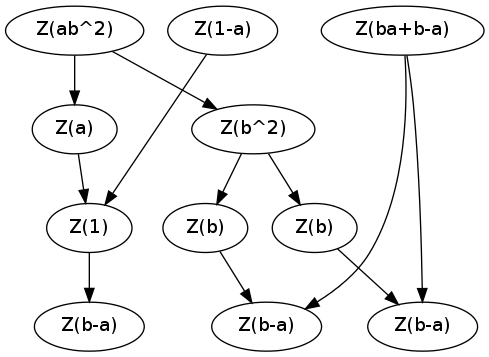
\includegraphics[scale=0.5]{dynamical-proof}
  \caption{\label{dynamical}Grafische Darstellung des Beispielbeweises.}
\end{figure}


\subsubsection*{Erweiterungen}

Satz~\ref{satz:genprime} hat gezeigt, dass man die klassische Vorgehensweise
\begin{quote}
\emph{Um zu zeigen, dass ein Element~$x \in R$ nilpotent ist, zeige, dass es in allen
Primidealen liegt.}\end{quote}
konstruktiv rechtfertigen kann -- obwohl konstruktiv nicht bewiesen werden
kann, dass der Schnitt aller Primideale nur die Menge der nilpotenten Elemente
ist. Klassisch gibt es aber auch noch folgendes stärkeres Prinzip:
\begin{lemma}[in dieser Form nur klassisch]\label{lemma:nullinabschl}%
Sei~$x \in R$ ein Element eines Rings~$R$. Wenn~$x$ in jedem algebraisch
abgeschlossenen Oberkörper von~$R$ Null ist, wenn also für jeden
Ringhomomorphismus~$\varphi : R \to K$, wobei~$K$ ein algebraisch
abgeschlossener Körper ist, das Element~$\varphi(x) \in K$ Null ist, dann
ist~$x$ nilpotent.\end{lemma}
In diesem Abschnitt wollen wir zeigen, dass auch dieses Prinzip
in einem konstruktiven Kontext verwendbar ist -- obwohl die Existenz
algebraischer Abschlüsse, und schon die Existenz von Zerfällungskörpern,
konstruktiv eine diffizile Angelegenheit ist. In diesem Abschnitt setzen wir
etwas mehr Vorwissen aus kommutativer Algebra voraus.

\begin{proof}[Beweis des Lemmas (nur klassisch)]
Wir weisen nach, dass~$x$ in allen Primidealen von~$R$ liegt, klassisch genügt
das ja. Sei also~$\pp$ ein beliebiges Primideal. Dann ist der
Faktorring~$R/\pp$ ein Integritätsbereich und wir können seinen
Quotientenkörper betrachten. Diesen wiederum können wir in einen algebraisch
abgeschlossenen Oberkörper~$K$ einbetten (hier geht klassische Logik ein). Wir
haben also Ringhomomorphismen
\[ R \longrightarrow R/\pp \lhra \Quot(R/\pp) \lhra K. \]
Nach Voraussetzung ist das Bild von~$x$ in~$K$ Null. Daher ist auch das Bild
von~$x$ in~$\Quot(R/\pp)$ Null, somit auch das Bild von~$x$ in~$R/\pp$, und
daher liegt~$x$ in~$\pp$.
\end{proof}

Die konstruktive Umsetzung dieses Prinzips im Rahmen der dynamischen Methoden
ist folgende:

\begin{satz}
Aus einem Beweis der Sequenz
\[ Z(a_1) \wedge \cdots \wedge Z(a_n) \seq{} Z(b) \]
welcher als sprachliche Mittel nur~$\top$, $\bot$, $\wedge$, $\vee$ sowie die
Quantoren, nicht aber~$\Rightarrow$, und als Schlussregeln
\begin{enumerate}
\item[1.] die Axiome aus Definition~\ref{defn:genprime} (jetzt in beliebigen
Kontexten, nicht nur im leeren),
\item[2.] $\top \seq{\vec x} Z(x) \vee \exists y{:}\, Z(1-xy)$,
\item[3.] $\top \seq{\vec x} \exists y{:}\, Z(y^n + a_{n-1}y^{n-1} + \cdots +
a_1y + a_0)$, und
\item[4.] die strukturellen Regeln, die Regeln für Konjunktion, Disjunktion,
Allquantifikation und Existenzquantifikation
\end{enumerate}
verwendet, kann man einen expliziten Zeugen der Aussage
\[ b \in \sqrt{(a_1,\ldots,a_n)} \subseteq R \]
extrahieren.
\end{satz}
\begin{proof}Wird nachgeliefert. Die Idee ist wieder, ein Modell anzugeben. Die
Interpretation einer Aussage im Kontext~$x_1,\ldots,x_n$ soll dabei ein
Radikalideal in~$R[x_1,\ldots,x_n]$ sein.\end{proof}
% XXX


\section{Ein topostheoretischer Zugang zu Quantenmechanik: der Bohr-Topos}

Als Anwendung konstruktiver Mathematik wollen wir einen topostheoretischen
Zugang zu (manchen Grundlagen von) Quantenmechanik vorstellen. Dieser geht auf
eine wegweisende Arbeit von Jeremy Butterfield, John Hamilton und Chris Isham
zurück~\cite{butterfield:hamilton:isham:1}, welche dann von weiteren
mathematischen Physikern, unter anderem Andreas Döring, Chris Heunen und Nicolaas
Landsman, und den konstruktiven Mathematikern Thierry Coquand und Bas Spitters
aufgegriffen wurde. Unsere Darstellung ist im Wesentlichen eine Zusammenfassung
der Artikel~\cite{topos:aqt} und~\cite{nlab:bohrtopos}. Ein genauerer Abriss
der Geschichte findet sich in~\cite{nlab:bohrtopos} und den dort genannten
Referenzen.

Die grundlegende Idee ist folgende:
Klassisch-mechanische Systeme können durch kommutative \csalgebren{} und
dazugehörige Phasenräume beschrieben werden. Die \csalgebra{} zu
quantenmechanischen Systemen ist dagegen im Allgemeinen nichtkommutativ und die
schöne Idee eines Phasenraums bricht zusammen. Man kann nun das das
mathematische Universum, in dem man arbeitet, wechseln; ein geeignetes
Alternativuniversum enthält ein Abbild der nichtkommutativen \csalgebra,
welches dort kommutativ erscheint und dort auch einen Phasenraum zulässt. In
diesem (restriktiven) Sinn wird Quantenmechanik in diesem anderen Universum zu
klassischer Mechanik.

Um diesen Ansatz zu verstehen, sind drei Zutaten nötig: die Dualität zwischen
Räumen und Algebren; eine für diese Zwecke geeignete Formulierung von
klassischer Mechanik und Quantenmechanik; und die Auffassung von Topoi als
mathematische Alternativuniversen. Diese Zutaten wollen wir in den folgenden
Abschnitten grob umreißen.


\subsection{Gelfand-Dualität zwischen topologischen Räumen und \csalgebren}

Grundlegend für das Wechselspiel zwischen Geometrie und Algebra ist folgende
Erkenntnis: Zu einem geometrischen Objekt~$X$ kann man die Menge der
(reellwertigen, komplexwertigen, allgemeineren) Funktionen auf~$X$ betrachten.
Diese Menge trägt algebraische Struktur (ist etwa ein Ring) und kann daher mit
Mitteln der Algebra untersucht werden. Dabei besteht die Hoffnung, dadurch
etwas über~$X$ zu lernen; in guten Fällen legt die Algebra von Funktionen
das geometrische Objekt~$X$ sogar schon eindeutig fest.

Dieses Motto hat in mehreren Teilgebieten der Mathematik konkrete Ausprägungen.
Etwa ist in algebraischer Geometrie folgende Proposition fundamental:
\begin{prop}Die Kategorie der affinen Schemata ist dual äquivalent zur Kategorie der
Ringe:
\[ \begin{array}{@{}rcl@{}}
  \textnormal{(Kat. der affinen Schemata)}^\op &\simeq& \textnormal{(Kat. der Ringe)} \\
  X &\mapsto& \Gamma(X, \O_X) = \textnormal{Ring der regulären Funktionen auf~$X$} \\
  \textnormal{Spektrum von~$A$} = \Spec A &\mapsfrom& A
\end{array} \]
\end{prop}

Für unsere Zwecke ist die \emph{Gelfand-Dualität} wichtig, die zwischen
kompakten Hausdorffräumen einerseits und \csalgebren{} andererseits vermittelt.
\begin{defn}Eine \csalgebra~$A$ ist ein Banachraum über~$\CC$ (also ein vollständiger
normierter Vektorraum über~$\CC$) zusammen mit einer
Multiplikationsoperation~$A \times A \to A$ und einer Involution~$(\freist)^* :
A \to A$, sodass gewisse natürliche Axiome erfüllt sind.\end{defn}
Prototypbeispiele für~\csalgebren{} sind~$\CC$ mit der komplexen Konjugation
als Involution und~$L(H,H) = \{ f : H \to H \,|\, \text{$f$ linear und stetig}
\}$ mit der Zuordnung~$f \mapsto f^\star$ (adjungierter Operator
zu~$f$) als Involution. Siehe~\cite{harpe:jones:cstar} für eine Einführung in
die Theorie der \csalgebren.
\begin{satz}[Gelfand-Dualität, so nur klassisch]
Die Kategorie der kompakten Hausdorffräume ist dual äquivalent zur Kategorie
der kommutativen~\csalgebren{} (mit Eins):
\[ \begin{array}{@{}rcl@{}}
  \textnormal{(Kat. der kompakten Hausdorffräume)}^\op &\simeq&
  \textnormal{(Kat. der kommutativen \csalgebren)} \\
  X &\mapsto& C(X, \CC) = \{ f : X \to \CC \,|\, \textnormal{$f$ stetig} \} \\
  \Spec A &\mapsfrom& A
\end{array} \]
Dabei wird~$C(X, \CC)$ vermöge der punktweisen Addition, Multiplikation und
Konjugation sowie der Supremumsnorm zu einer~\csalgebra. Die Punkte von~$\Spec
A$ sind genau die \csalgebren{}homomorphismen~$A \to \CC$.
\end{satz}
\begin{proof}
Führt hier zu weit. Wir wollen nur anmerken, dass der Homöomorphismus~$X \to
\Spec C(X,\CC)$ durch~$x \longmapsto \freist(x)$ mit~$\freist(x) = (f \mapsto
f(x))$ gegeben ist. An einer Stelle im Beweis muss man geeignete
Algebrenhomomorphismen~$A \to \CC$ konstruieren; dazu benötigt man das
Auswahlaxiom.
\end{proof}

Unter der Korrespondenz des Satzes entsprechen die selbstadjungierten
Elemente~$a \in A$ gerade den stetigen Abbildungen~$X \to \RR$.

\begin{bem}Die Gelfand-Dualität liefert einen Ansatz für \emph{nichtkommutative
Geometrie}: Wie man die Definition eines topologischen Raums abändern sollte,
sodass sie nicht mehr "`kommutativ"' wäre, ist völlig unklar, denn in
der Definition kommen ja gar keine binären Verknüpfungen vor. Auf der algebraischen Seite
ist es dagegen einfach. Daher kann man das formale Duale zur Kategorie der
(nicht notwendigerweise kommutativen) \csalgebren{} als erste Approximation für
eine Kategorie nichtkommutativer Räume verwenden.
\end{bem}


\subsection{Örtlichkeiten für punktfreie Topologie}

In der obigen Formulierung gilt die Gelfand-Dualität leider nur in einem
klassischen Kontext. Da wir sie später in einem alternativen
Mathematik-Universum (dem Bohr-Topos zu einer nichtkommutativen \csalgebra)
nutzen wollen, in dem das Auswahlaxiom unabhängig von unseren philosophischen
Vorlieben schlichtweg \emph{nicht gilt}, ist das unzureichend. Im Zeitraum von
etwa 20~Jahren wurde glücklicherweise auch folgende konstruktiv zulässige Variante
entwickelt:

\begin{satz}[auch konstruktiv]Die Kategorie der kompakten und vollständig
regulären Örtlichkeiten (Locales) ist dual äquivalent zur Kategorie der
kommutativen~\csalgebren. Dabei geht analog zur klassischen Formulierung eine
Örtlichkeit~$X$ auf die Algebra der stetigen Abbildungen~$X \to \CC$.
(Auf die hierfür nötige konstruktiv geeignete Definition der komplexen Zahlen
gehen wir nicht ein.)
\end{satz}

Dabei ist das Konzept einer \emph{Örtlichkeit} (Locale) eine milde
Verallgemeinerung des Konzepts eines topologischen Raums, bei dem \emph{Punkte}
nicht im Vordergrund stehen: Während ein topologischer Raum bekanntlich durch
eine Menge von Punkten sowie der Deklaration gewisser Mengen von Punkten als
offen gegeben ist, besteht eine Örtlichkeit nur aus der Angabe von
gewissen \emph{offenen Dingen}, welche nicht notwendigerweise Mengen von
Punkten sein müssen. Von den offenen Teilmengen eines topologischen Raums
schaut man sich die Axiome ab, die die offenen Dinge einer Örtlichkeit
erfüllen sollen:

\begin{defn}Eine \emph{Örtlichkeit}~$X$ besteht aus einem Verband~$\Ouv(X)$
\emph{offener Dinge} (also einer Halbordnung zusammen mit Operationen~$\wedge$
und~$\vee$, die geeignete Axiome erfüllen), in dem zusätzliche beliebige
Suprema existieren und für diese folgendes Distributivitätsgesetz gilt:
\[ u \wedge \bigvee_i v_i = \bigvee_i (u \wedge v_i). \]
\end{defn}

\begin{bsp}
Jeder topologischer Raum~$X$ liefert ein Beispiel für eine Örtlichkeit~$X$
mit~$\Ouv(X) = \{ U \subseteq X \,|\, \text{$U$ offen} \}$ und~$\wedge =
\cap$, $\vee = \cup$, $\bigvee = \bigcup$.\end{bsp}

\begin{bsp}Speziell ist der einpunktige Raum~$\pt$ als Örtlichkeit
durch~$\Ouv(\pt) = \P(\{\star\})$ gegeben.\end{bsp}

Das Konzept eines Punkts ist in der Theorie der Örtlichkeiten nicht
grundlegend, kann aber sehr wohl definiert werden: Ein \emph{Punkt} einer
Örtlichkeit~$X$ ist ein Morphismus~$\pt \to X$ von Örtlichkeiten. Die Menge
aller Punkte einer Örtlichkeit kann man mit einer natürlichen Topologie
versehen; der so entstehende topologische Raum spiegelt aber nur dann die
Örtlichkeit getreu wieder, wenn diese \emph{räumlich} war. Insbesondere gibt es
nichttriviale und interessante Örtlichkeiten, die keinen einzigen Punkt
besitzen: Die Vorstellung eines Punkts ist gewissermaßen ein ideelles und
schwerer fassbares Konzept als das eines offenen Teils eines Raums. Auch, wenn
es einem Raum an Punkten mangelt, kann man manchmal dennoch von offenen
Teilbereichen sprechen.

\begin{bsp}Folgende Örtlichkeiten sind nichttrivial und besitzen keine Punkte:
die Örtlichkeit aller Surjektionen~$\NN \twoheadrightarrow \RR$, die
Örtlichkeit aller zufälligen~$0/1$-Folgen, der örtlichkeitstheoretische Schnitt
beliebig vieler dichter Unterörtlichkeiten einer nichttrivialen Örtlichkeit.\end{bsp}

Umgekehrt spiegelt auch die Örtlichkeit zu einem topologischen Raum diesen nur
dann getreu wieder, wenn dieser \emph{nüchtern} war. Jeder Hausdorffraum ist
nüchtern (in klassischer Logik).
Stattet man aber etwa eine aus mehr als nur einem Element bestehende Menge 
mit der indiskreten Topologie aus, erhält man einen
topologischen Raum, der nicht nüchtern ist: Die Vielzahl seiner Punkte schlägt
sich nicht in seiner Topologie nieder. Seine \emph{Nüchternifizierung}
(\emph{Ausnüchterung}?) ist der einpunktige Raum.

Hier ist nicht der richtige Ort, um auf die vielen Vorteile (und die Nachteile) von
Örtlichkeiten gegenüber topologischen Räumen einzugehen. Es sei nur erwähnt,
dass durch den Wegfall von Punkten als grundlegendes Konzept diese auch
seltener konstruiert werden müssen. Da man zur Angabe spezieller Punkte oft das
Auswahlaxiom oder andere klassische Prinzipien benötigt, eignen sich
Örtlichkeiten also besser, wenn man solche nicht verwenden möchte oder (wie bei
der Arbeit in anderen Topoi) nicht verwenden kann.

Wir wollen mit einem Zitat von Alexander Grothendieck über
Topoi~\cite{grothendieck:zitat}, das aber
genauso gut auf Örtlichkeiten anwendbar ist, schließen:\footnote{%
"`Diese \glq Wahrscheinlichkeitswolken\grq, welche die beruhigenden materiellen
Partikel von früher ersetzen, erinnern mich irgendwie an die flüchtigen
\glq offenen Umgebungen\grq{} der Topoi -- wie dahinschwindende Phantome, um
die fiktiven \glq Punkte\grq{} zu umgeben, [\ldots]."'}
\begin{quote}
\selectlanguage{french}
Ces “nuages probabilistes”, remplaçant les rassurantes particules matérielles
d’antan, me rappellent étrangement les élusifs “voisinages ouverts” qui
peuplent les topos, tels des fantômes évanescents, pour entourer des “points”
imaginaires, [\ldots].
\end{quote}


\subsection{Algebraische Sicht auf klassische Mechanik und Quantenmechanik}

\subsubsection*{Klassische Mechanik}

Zu einem klassisch-mechanischen System gehört ein Phasenraum~$\Sigma$, dessen
Punkte die reinen Zustände des Systems sind.

\begin{bsp}Der Phasenraum des freien Teilchens im~$\RR^3$ ist~$\Sigma = \RR^3
\times \RR^3$, denn durch Position und Impuls ist die Systemkonfiguration
eindeutig festgelegt. Die beiden Projektionen~$\Sigma \to \RR^3$ sind die
Observablen \emph{Position} und \emph{Impuls}.\end{bsp}

Auf der algebraischen Seite gehört zum Phasenraum~$\Sigma$ eine \csalgebra~$A
:= C(\Sigma, \CC)$; es ergibt sich dann folgendes Wörterbuch zwischen
Formulierungen auf der geometrischen und der algebraischen
Seite~\cite{nlab:classmech}:

\begin{itemize}
\item \emph{Reine Zustände} sind Punkte~$x \in \Sigma$ oder, da~$\Sigma \cong \Spec
A$, äquivalent \csalgebren{}\-ho\-mo\-mor\-phis\-men $A \to \CC$.

\item \emph{Gemischte Zustände} sind Wahrscheinlichkeitsmaße~$\mu$ auf~$\Sigma$ oder
äquivalent lineare Abbildungen~$\rho : A \to \CC$, welche normiert
(d.\,h.~$\rho(1) = 1$) und positiv sind (d.\,h.~$\rho(a^\star a) \geq 0$
für alle~$a \in A$). (Solche Abbildungen sind automatisch stetig.)

Der Zusammenhang zwischen den beiden Sichtweisen wird durch
\[ \rho(f) = \int_\Sigma f(x) \,d\mu(x) \]
für alle~$f \in A$ gegeben: Ein Wahrscheinlichkeitsmaß~$\mu$ definiert über
diese Setzung eine normierte, positive und lineare Abbildung; dass umgekehrt
jedes solche Funktional von dieser Form ist, garantiert der Darstellungssatz
von Riesz-Markov-Kakutani.

Unter dieser Korrespondenz entspricht ein reiner Zustand~$x \in \Sigma$ dem
in~$x$ konzentrierten Dirac-Maß bzw. der Abbildung~$\rho$ mit~$\rho(f) =
f(x)$.

\item \emph{Observable} sind stetige Funktionen~$\Sigma \to \RR$ oder
äquivalent selbstadjungierte Elemente~$a \in A$.

Eine spezielle Observable ist die Eins von~$A$, also die Funktion, die konstant
den Wert~$1 \in \RR$ annimmt.

\item Der Erwartungswert einer Observablen~$a$ in einem Zustand~$\rho$
ist~$\rho(a)$. Ist~$\rho$ durch ein Wahrscheinlichkeitsmaß~$\mu$ gegeben,
lässt sich dieser Ausdruck auch als~$\int_\Sigma a(x) \,d\mu(x)$ schreiben;
diese Form ist vielleicht vertrauter.

Die Forderung, dass~$\rho$ normiert ist, ist dann anschaulich: Denn der
Erwartungswert der konstanten Observable~$1 \in A$ sollte auch tatsächlich~$1$
sein.

Ist~$\rho = \freist(x)$ ein reiner Zustand, so ist~$\rho(a) = a(x)$ nicht nur
der Erwartungswert, sondern der tatsächliche Wert von~$a$.
\end{itemize}

\begin{bem}In Anwendungen ist der Phasenraum sogar eine
(Poisson"~)""Mannigfaltigkeit. Diese zusätzliche Struktur sollte man nicht
ignorieren. Machen wir hier aber trotzdem.\end{bem}


\subsubsection*{Quantenmechanik}

Quantenmechanische Systeme können nicht mehr durch einen Phasenraum im
traditionellen Sinn beschrieben werden. Es bleibt aber die Möglichkeit, sie
durch nichtkommutative~\csalgebren{} zu beschreiben.

\begin{bsp}Wird ein System durch einen Hilbertraum~$H$ beschrieben, so ist~$A
:= L(H,H) = \{ f : H \to H \,|\, \text{$f$ linear und stetig} \}$ die
zugehörige~\csalgebra.\end{bsp}

Grundlegende Konzepte können also nicht mehr geometrisch über einen Phasenraum
verstanden werden, sondern müssen algebraisch formuliert werden. In Analogie
zur klassischen Situation könnte man definieren:
\begin{itemize}
\item \emph{Reine Zustände} sind \csalgebren{}\-homo\-mor\-phis\-men~$A \to
\CC$.
\item \emph{Gemischte Zustände} sind normierte, positive und lineare
Abbildungen~$A \to \CC$.
\item \emph{Observablen} sind selbstadjungierte Elemente von~$A$.
\item Der Erwartungswert einer Observablen~$a$ in einem Zustand~$\rho$
ist~$\rho(a)$.
\end{itemize}

\begin{bsp}Jeder reine Zustand ist auch ein gemischter Zustand, da
\csalgebren{}\-homo\-mor\-phis\-men~$\rho : A \to \CC$ automatisch normiert (da sie das
Einselement auf die komplexe Zahl~$1$ schicken müssen) und positiv sind
(da~$\rho(a^* a) = \rho(a)^* \rho(a) = |\rho(a)|^2 \geq 0$).\end{bsp}

\begin{bsp}\begin{itemize}
\item Ist~$\psi \in H$ eine normierte Wellenfunktion, so ist~$\rho$
mit~$\rho(a) = (\psi, a(\psi))$ ein gemischter Zustand, im Allgemeinen aber
kein reiner.
\item Ist~$(\psi_i)_i$ eine Familie normierter Wellenfunktionen und~$(p_i)_i$
eine Familie nichtnegativer Zahlen mit~$\sum_i p_i = 1$, so ist~$\rho$
mit~$\rho(a) = \sum_i p_i \cdot (\psi_i, a(\psi_i))$ ein gemischter Zustand.
\item Ist~$a : H \to H$ ein selbstadjungierter Operator, so ist~$a \in A$ eine
Observable.
\end{itemize}
\end{bsp}

Bei näherer Betrachtung stellt sich dieser Ansatz jedoch als zu naiv heraus. Das
Problem steckt in der unscheinbaren Bedingung
\[ \rho(a + b) = \rho(a) + \rho(b) \quad\text{für alle~$a,b \in A$} \]
an gemischte Zustände~$\rho$ bzw. der analogen Forderung der
Multiplikativität an reine Zustände. Man kann nämlich
argumentieren~\cite[Seite~27]{topos:aqt},
dass zwei Observable~$a$ und~$b$ nur dann physikalisch sinnvoll addierbar sind,
wenn sie gemeinsam messbar sind, also miteinander kommutieren. Die
mathematischen Physiker, die nicht nur vorgeben, sich mit diesem Thema
auszukennen, begründen das mit einer Referenz auf Bohrs \emph{Doktrin
klassischer Konzepte}, auf die wir weiter unten eingehen. Jedenfalls sollte man
besser folgende Definition treffen:

\begin{defn}\begin{enumerate}
\item
Ein \emph{reiner Quasi-Zustand} einer \csalgebra~$A$ ist eine Abbildung~$A \to \CC$,
die auf jeder kommutativen Unter-\csalgebra~$C \subseteq A$ ein
\csalgebren\-homo\-mor\-phis\-mus ist.
\item Ein \emph{gemischter Quasi-Zustand} einer \csalgebra~$A$ ist eine Abbildung~$A
\to \CC$, welche normiert, positiv und auf jeder kommutativen
Unter-\csalgebra~$C \subseteq A$ linear ist.
\end{enumerate}
\end{defn}

\begin{bem}In der Praxis ist der Unterschied zwischen Zuständen und den besser
motivierten Quasi-Zuständen nicht so groß: Denn nach Gleasons Theorem ist jeder
gemischte Quasi-Zustand auf~$A = L(H,H)$ mit~$\dim H \geq 3$ schon ein
gemischter Zustand.\end{bem}

\begin{bem}\label{bem:keine-reinen-quasi-zustaende}%
Es gibt einen Grund, wieso wir kein Beispiel eines reinen Quasi-Zustands
angeführt haben: Das Kochen-Specker-Theorem besagt, dass es zumindest im
interessanten Fall~$A = L(H,H)$ mit~$\dim H \geq 3$ keinen solchen gibt. Das
hat eine physikalische Interpretation: Ein reiner Quasi-Zustand würde allen
Observablen konsistente Zahlenwerte als Messwerte zuweisen. So etwas ist nicht
möglich.\end{bem}


\subsection{Topoi als mathematische Alternativuniversen}

\label{sect:topoi}%
Topostheorie hat viele Facetten. Hier betonen wir nur eine, nämlich
die Auffassung von Topoi als mathematische Alternativuniversen. Unter anderem
hat Topostheorie aber auch eine geometrische Komponente: Topoi kann man als
verallgemeinerte Räume ansehen. Eine informale Einführung in Topostheorie
von Tom Leinster~\cite{leinster:topos} diskutiert auch diese anderen
Standpunkte.

In diesem und im folgenden Abschnitt setzen wir etwas Grundkenntnisse in
Kategorientheorie voraus. Alle benötigten Konzepte kann man etwa im
Skript zum vorherigen Pizzaseminar~\cite{pizzaseminar:kategorientheorie}
nachlesen. Gelegentlich werden wir auch über Garben sprechen; die wesentlichen
Definitionen dazu sind in Anhang~\ref{appendix:garben} zusammengestellt. Man
kann solche Passagen aber auch überlesen.


\subsubsection*{Was ist ein Topos?}

\begin{defn}Ein \emph{Topos} ist eine Kategorie, die endliche Limiten besitzt,
kartesisch abgeschlossen ist und über einen Unterobjektklassifizierer verfügt.
\end{defn}

Notwendig und hinreichend für die Existenz endlicher Limiten ist die Existenz
eines terminalen Objekts (eines Objekts~$1$, sodass für jedes Objekt~$X$ genau
ein Morphismus~$X \to 1$ existiert), von Produkten~$X \times Y$ für je zwei
Objekte~$X$ und~$Y$ und von Differenzkernen für je zwei parallele Morphismen~$X
\to Y$.

\emph{Kartesisch abgeschlossen} bedeutet, dass es zu je zwei Objekten~$X$
und~$Y$ nicht nur wie in jeder Kategorie eine Menge (oder Klasse)~$\Hom(X,Y)$
von Morphismen zwischen~$X$ und~$Y$ gibt, sondern dass man sinnvoll von einem
internen \emph{Hom-Objekt}~$\underline{\Hom}(X,Y)$ der Kategorie sprechen kann.
Das ist etwa in der Kategorie der Mengen und beinahe in der Kategorie der
topologischen Räume der Fall (da man die Hom-Mengen mit einer Topologie
versehen kann).

Ein \emph{Unterobjektklassifizierer} ist ein spezielles Objekt~$\Omega$, sodass
Unterobjekte eines Objekts~$X$ in 1:1-Korrespondenz zu Morphismen~$X \to
\Omega$ stehen. In der Kategorie der Mengen ist~$\Omega = \P(\{\star\})$ ein solches, in
klassischer Logik also~$\Omega = \{ 0, 1 \}$: Denn bekanntlich
können Teilmengen~$U$ einer Menge~$X$ ja eindeutig durch ihre klassifizierende
Abbildung~$X \to \Omega,\ x \mapsto \{ \star \,|\, x \in U \}$ (also~$x \mapsto
1$, falls~$x \in U$, und~$x \mapsto 0$, falls~$x \not\in U$) beschrieben
werden.

Obige Definition ist völlig korrekt, für unsere Zwecke aber aus zwei
Gründen nicht gut geeignet: Zum einen ist sie nur dann anschaulich
verständlich, wenn man schon einige Erfahrung mit Kategorientheorie hat. Zum
anderen ist sie in einem gewissen Sinn sogar irreführend, denn ein Topos hat
viel mehr Struktur, als die auf Minimalität getrimmte Definition vermuten ließe.
Eine umfassendere Definition, die diese weiteren wesentlichen Strukturen nicht
verschweigt, ist etwa folgende: Ein \emph{Topos} ist eine lokal kartesisch
abgeschlossene, endlich vollständige und kovollständige Heyting-Kategorie,
welche exakt und extensiv ist und über einen Unterobjektklassifizierer verfügt.

Für unsere Zwecke genügen ein Motto und Beispiele für Topoi.

\begin{motto}Ein Topos ist eine Kategorie, die dadurch, dass sie ähnliche
kategorielle Eigenschaften wie die Kategorie der Mengen hat, über eine
\emph{interne Sprache} verfügt.\end{motto}

\begin{bsp}Archetypisches Beispiel für einen Topos ist die Kategorie~$\Set$ der
Mengen und Abbildungen.
\end{bsp}

\begin{bsp}Ist~$X$ ein topologischer Raum (oder eine Örtlichkeit), so ist die
Kategorie der mengenwertigen Garben über~$X$ und der Garbenmorphismen ein
Topos. Das terminale Objekt ist die konstante Garbe~$U \mapsto \{ \star \}$,
das initiale die Garbe~$U \mapsto \{ \star \,|\, U = \emptyset \}$ und der
Unterobjektklassifizierer ist die Garbe~$U \mapsto \{ V \subseteq U \,|\,
\text{$V$ offen} \}$.
\end{bsp}

\begin{bsp}Die Kategorien der Gruppen, der Vektorräume und der topologischen Räume sind
keine Topoi.\end{bsp}


\subsubsection*{Was ist die interne Sprache?}

Die interne Sprache eines Topos~$\E$ erlaubt es,
Objekte und Morphismen des Topos zu konstruieren,
Eigenschaften über diese zu formulieren und
gegebenenfalls solche Eigenschaften zu beweisen --
und zwar in einer \emph{naiven}, \emph{element-basierten} Sprache, die der
üblichen formalen mathematischen Sprache sehr stark ähnelt.

Etwa erscheint ein Objekt von~$\E$, das also vielleicht eine komplizierte Garbe
von Mengen ist, aus Sicht der internen Sprache wie eine gewöhnliche
Menge\footnote{Besser sollte man hier \emph{Typ} schreiben. Auf den
Unterschied wollen wir hier nicht eingehen.}. Folgerichtig erscheint ein
Morphismus von~$\E$, der tatsächlich vielleicht ein Garbenmorphismus und daher
eine komplizierte unendliche
Familie von Abbildungen ist, aus Sicht der internen Sprache wie eine
gewöhnliche Abbildung zwischen Mengen.

Diese Auffassung ist sehr tragfähig: Etwa sieht das initiale Objekt aus Sicht
der internen Sprache auch in der Tat wie die leere Menge, ein Monomorphismus
wie eine injektive Abbildung und ein Epimorphismus wie eine surjektive
Abbildung aus, siehe Tafel~\ref{tafel:externintern}.

Wichtige Eigenschaft der internen Sprache ist, dass sie \emph{korrekt} (engl.
\emph{sound}) bezüglich konstruktiver Logik ist. Jeder konstruktive Beweis
lässt sich also auch in der internen Sprache beliebiger Topoi interpretieren.
Im Folgenden Abschnitt illustrieren wir das anhand des anschaulichen
Garbentopos zu einem topologischen Raum.

\begin{table}
  \centering
  \small
  \setlength{\extrarowheight}{0.3em}
  \begin{tabular}{@{}r|l@{}}
    externe Sicht & interne Sicht
    \\\hline
    Objekt von~$\E$ & gewöhnliche Menge \\
    Morphismus von~$\E$ & gewöhnliche Abbildung zwischen Mengen \\
    initiales Objekt von~$\E$ & leere Menge \\
    terminales Objekt von~$\E$ & einelementige Menge \\
    Unterobjektklassifizierer von~$\E$ & Menge~$\P(\{\star\})$ der
    Wahrheitswerte \\
    Monomorphismus in~$\E$ & injektive Abbildung \\
    Epimorphismus in~$\E$ & surjektive Abbildung
  \end{tabular}
  \caption{\label{tafel:externintern}Externe und interne Sicht auf Objekte und
  Morphismen eines Topos~$\E$}
\end{table}


\subsubsection*{Die interne Sprache eines Garbentopos}

\label{internesprache}%
Sei~$X$ ein topologischer Raum (oder eine Örtlichkeit). Dann definieren wir rekursiv
\[ U \models \varphi \quad \text{("`$\varphi$ gilt auf~$U$"')} \]
für offene Teilmengen~$U \subseteq X$ und Aussagen~$\varphi$ gemäß
der Regeln in Tafel~\ref{tafel:kripke-joyal} (der
\emph{Kripke-Joyal-Semantik}).

\begin{table}
  \centering
  \small
  \setlength{\extrarowheight}{0.3em}
  \newcommand{\Ll}{:\Longleftrightarrow}
  \[ \renewcommand{\arraystretch}{1.3}\begin{array}{@{}lcl@{}}
    U \models f = g \? \F &\Ll& f|_U = g|_U \in \Gamma(U, \F) \\
    U \models \top &\Ll& \text{$U = U$ (gilt stets)} \\
    U \models \bot &\Ll& U = \emptyset \\
    U \models \varphi \wedge \psi &\Ll&
      \text{$U \models \varphi$ und $U \models \psi$} \\
    U \models \varphi \vee \psi &\Ll&
      \hcancel{\text{$U \models \varphi$ oder $U \models \psi$}}{0pt}{3pt}{0pt}{-2pt} \\
    && \text{es gibt eine Überdeckung $U = \bigcup_i U_i$ sodass für alle~$i$:} \\
    && \quad\quad \text{$U_i \models \varphi$ or $U_i \models \psi$} \\
    U \models \varphi \Rightarrow \psi &\Ll&
      \text{für alle offenen~$V \subseteq U$: } 
    \text{$V \models \varphi$ impliziert $V \models \psi$} \\
    U \models \forall f \? \F\_ \varphi(f) &\Ll&
      \text{für alle Schnitte~$f \in \Gamma(V, \F), V \subseteq U$: $V \models
      \varphi(f)$} \\
    U \models \exists f \? \F\_ \varphi(f) &\Ll&
      \hcancel{\text{es gibt einen Schnitt~$f \in \Gamma(U, \F)$ mit~$U \models
      \varphi(f)$}}{0pt}{3pt}{0pt}{-2pt} \\
    &&
      \text{es gibt eine Überdeckung $U = \bigcup_i U_i$ sodass für alle~$i$:} \\
    && \quad\quad \text{es gibt~$f_i \in \Gamma(U_i, \F)$ sodass
    $U_i \models \varphi(f_i)$}
  \end{array} \]
  \vspace{-1.5em}
  \caption{\label{tafel:kripke-joyal}Die Kripke-Joyal-Semantik eines
  Garbentopos~$\Sh(X)$.}
\end{table}

\begin{bsp}Seien~$s,t \in \Gamma(X, \F)$ globale Schnitte einer Garbe~$\F$.
Dann gilt~$U \models s = t$ genau dann, wenn~$s|_U = t|_U$, und~$U \models
\neg\neg(s = t)$ genau dann, wenn es eine dichte offene Teilmenge~$V \subseteq
U$ mit~$s|_V = t|_V$ gibt.\end{bsp}

Auf den ersten Blick erscheinen die Regeln der Kripke-Joyal-Semantik völlig
willkürlich. Tatsächlich sind sie aber fein aufeinander abgestimmt, schon
kleine Änderungen führen dazu, dass das gesamte System zusammenbricht. Nur so
gilt folgende grundlegende Proposition:

\begin{satz}\label{soundness}%
Die interne Sprache von~$\Sh(X)$ hat folgende Eigenschaften:
\begin{enumerate}
\item \emph{Lokalität:} Sei~$U = \bigcup_i U_i$ eine offene Überdeckung. Dann
gilt genau dann~$U \models \varphi$, wenn für alle~$i$ jeweils~$U_i \models
\varphi$ gilt.
\item \emph{Korrektheit:} Wenn~$U \models \varphi$ und
intuitionistisch~$\varphi \seq{} \psi$ ableitbar ist, dann gilt auch~$U \models
\psi$.
\end{enumerate}
\end{satz}

Diese Proposition ist der Grund für die Nützlichkeit der internen Sprache: Wenn
man eine garbentheoretische Implikation~$A \Rightarrow B$ beweisen möchte, kann man vielleicht
Voraussetzung und Behauptung als Interpretationen gewisser naiv-sprachlicher
Aussagen~$\tilde A$ bzw.~$\tilde B$ mit der Kripke-Joyal-Semantik erkennen. Um
dann die Implikation zu beweisen, genügt es, in naiver Sprache einen
konstruktiven Beweis von~$\tilde A \Rightarrow \tilde B$ zu führen.

\begin{bsp}In einer Grundvorlesung zeigt man, dass die Verkettung surjektiver
Abbildungen wieder surjektiv ist. Da der Beweis konstruktiv ist, folgt durch
Interpretation im Garbentopos daraus sofort, dass die Verkettung von
Epimorphismen von Garben wieder ein Epimorphismus ist. Der Beweis der Aussage, dass jede
surjektive Abbildung~$f$ einen Schnitt~$g$ (eine Abbildung in die umgekehrte
Richtung mit~$g \circ f = \id$) zulässt, erfordert dagegen das Auswahlaxiom und
lässt sich daher nicht in der internen Sprache interpretieren; tatsächlich
haben Epimorphismen von Garben auch nur in den seltensten Fällen Rechtsinverse.\end{bsp}

\begin{bsp}Nur um Neugierde zu wecken hier ein komplexeres Beispiel:
Konstruktiv kann man nicht zeigen, dass jeder endlich erzeugte Vektorraum über
einem Körper eine Basis besitzt. Das liegt nicht etwa daran, dass solche
plötzlich unendlichdimensional werden, sondern schlichtweg daran, dass man
konstruktiv keine Basis explizit angeben kann. Man kann aber die schwächere
Behauptung zeigen, dass jeder endlich erzeugte Vektorraum \emph{nicht nicht}
eine Basis besitzt. Diese Aussage zieht durch Interpretation im
Garbentopos~$\Sh(X)$ eines reduzierten Schemas~$X$ sofort folgendes Korollar
nach sich: Jeder~$\O_X$-Modul, der lokal von endlichem Typ ist, ist zwar nicht
unbedingt lokal frei, aber zumindest auf einer dichten offenen Teilmenge lokal
frei. (Die Reduziertheitsvoraussetzung geht insofern ein, als dass~$\O_X$ aus
Sicht der internen Sprache genau dann ein geeignetes Körperaxiom erfüllt,
wenn~$X$ reduziert ist.)\end{bsp}

\begin{aufg}Sei~$\alpha : \F \to \G$ ein Morphismus von Garben auf~$X$. Zeige:
\begin{enumerate}
\item
Der Morphismus~$\alpha$ ist genau dann ein Monomorphismus von Garben, wenn
$X \models \forall x,y\?\F\_ \alpha(x) = \alpha(y) \Rightarrow x = y$.
\item
Der Morphismus~$\alpha$ ist genau dann ein Epimorphismus von Garben, wenn
$X \models \forall y\?\G\_ \exists x\?\F\_ \alpha(x) = y$.
\end{enumerate}
\end{aufg}

\begin{bem}In dem Garbentopos eines ($\text{T}_1$-)Raums~$X$ gilt genau dann das Prinzip
vom ausgeschlossenen Dritten, wenn~$X$ diskret ist. Das ist ein langweiliger
Fall. Garbentopoi zu interessanten topologischen Räumen liefern also einen
völlig sachlichen Grund, wieso es nützlich ist, sich mit konstruktiver Logik zu
beschäftigen.
\end{bem}

\subsubsection*{Kann man mit der Topossprache Sätze beweisen, die man ohne sie
nicht beweisen könnte?}

Im Beweis von Satz~\ref{soundness} ist ein Verfahren versteckt, wie man aus
jedem intern geführten Beweis einen Beweis der entsprechenden übersetzten
Aussagen im gewöhnlichen extern Sinn gewinnen kann. Daher kann man mit der
Topossprache sicherlich \emph{nicht} Sätze beweisen, die man ohne sie nicht
beweisen könnte.

Allerdings kann es sehr viel einfacher sein, in der internen Welt zu denken und
zu arbeiten. Dieser Vorteil ist nicht zu unterschätzen: Wenn man sich etwa
einmalig ein Wörterbuch zwischen externen Begriffen der algebraischen Geometrie
und zugehörigen internen Begriffen geeigneter Topoi anlegt, kann man fortan
viele Beweise von grundlegenden Aussagen kurz und konzeptionell
führen, anstatt wie sonst mit affinen Überdeckungen, Übergang zu Halmen
und ähnlichen Techniken hantieren zu müssen.


\subsection{Der Bohr-Topos zu einer nichtkommutativen \csalgebra}

Sei~$A$ die nichtkommutative \csalgebra{} eines quantenmechanischen Systems.

\begin{defn}\begin{enumerate}
\item
Ein \emph{klassischer Kontext} von~$A$ ist eine kommutative Unter-\csalgebra~$C
\subseteq A$.
\item Die bezüglich der Inklusion geordnete Menge aller klassischen Kontexte
von~$A$ sei~$\C(A)$.
\end{enumerate}
\end{defn}

Die Idee hinter dieser Namensgebung ist folgende: Die Observablen
(selbstadjungierten Elemente) einer kommutativen Unteralgebra~$C \subseteq
L(H,H)$ lassen sich \emph{simultan} diagonalisieren und erlauben daher einen
konsistenten Satz von Messwerten -- ohne, dass Heisenbergs Unschärferelation in
die Quere kommt.

\begin{defn}Der \emph{Bohr-Topos} zur \csalgebra~$A$ ist die Koprägarbenkategorie
\[ \Bohr(A) := [\C(A), \Set] \]
aller Funktoren~$\C(A) \to \Set$ und natürlichen Transformationen zwischen
ihnen.\footnote{Äquivalent kann man den Bohr-Topos auch als den Garbentopos
über~$A$, versehen mit der Alexandroff-Topologie, auffassen: Die offenen Mengen
sind dabei die nach oben abgeschlossenen Teilmengen, und eine Basis der
Topologie ist durch die Teilmengen der Form~${\uparrow}(C) := \{ C' \in \C(A)
\,|\, C \subseteq C' \}$ für~$C \in \C(A)$ gegeben. Unter dieser Äquivalenz
induziert eine Garbe~$F$ auf diesem
Raum einen Funktor~$\C(A) \to \Set$ durch die Setzung~$C \mapsto
F({\uparrow}(C))$.}
\end{defn}

Ein solcher Funktor~$F : \C(A) \to \Set$ ordnet auf konsistente Art und Weise
jedem klassischen Kontext~$C \subseteq A$ eine Menge~$F(C)$ zu. Gewissermaßen
setzt daher der Topos solcher Funktoren Bohrs Doktrin klassischer Konzepte um
-- in Bohrs eigenen Worten~\cite[Seite~209]{bohr} (Hervorhebung im
Original)\footnote{"`\emph{Inwieweit auch
die Phänomene die Grenzen klassischer physikalischer
Erklärungen sprengen, die Darstellung aller Anhaltspunkte muss trotzdem
in klassischer Sprache ausgedrückt werden.} Das Argument ist einfach:
Mit dem Wort \glq Experiment\grq{} drücken wir eine Situation aus, in der wir
anderen erzählen können, was wir getan und gelernt haben. Deshalb müssen
Versuchsanordnung und Beobachtungsresultate in
unmissverständlicher Sprache ausgedrückt werden -- unter passender
Anwendung der Terminologie klassischer Physik."'}:
\begin{quote}
\selectlanguage{english}
[\ldots] \emph{however far the phenomena transcend the scope of classical physical
explanation, the account of all evidence must be expressed in
classical terms.} The argument is simply that by the word ``experiment''
we refer to a situation where we can tell others what we
have done and what we have learned and that, therefore, the account of
the experimental arrangements and of the results of the observations
must be expressed in unambiguous language with suitable application of
the terminology of classical physics.
\end{quote}

\begin{bem}Wer die Definition von Garben auf topologischen Räumen~$X$ als
Funktoren~$\Ouv(X)^\op \to \Set$
kennt, findet die unterschiedliche Wahl der Varianz an dieser Stelle vielleicht
überraschend. Tatsächlich aber ist diese zu erwarten: Offene Mengen werden umso
interessanter, je kleiner sie werden, da sie dann genauere Information über die
Lage ihrer enthaltenen Punkte vermitteln. Kommutative Unteralgebren werden
dagegen umso interessanter, je größer sie werden, denn für Elemente wird
es umso schwerer, miteinander zu kommutieren, je mehr sie werden. Man bedenke auch, dass
beliebige Vereinigungen (aber nicht beliebige Schnitte) offener Mengen offen
sind, und dass umgekehrt beliebige Schnitte (aber nicht beliebige
Summen) kommutativer Unteralgebren kommutativ sind.\end{bem}

Die nichtkommutative \csalgebra~$A$ besitzt nun ein Abbild~$\ul{A}$ im
Bohr-Topos. Diese \emph{interne} \csalgebra{} ist \emph{kommutativ}. In diesem
(restriktiven) Sinn wird Quantenmechanik bei interner Betrachtung zu klassischer
Mechanik.

\begin{defn}Die tautologisch definierte Koprägarbe
\[ \begin{array}{@{}rrcl@{}}
  \ul{A}:\ & \C(A) &\longrightarrow& \Set \\
  & C &\longmapsto& C
\end{array} \]
heißt \emph{Bohrifizierung} von~$A$.\end{defn}
\begin{prop}Die Bohrifizierung von~$A$
ist aus der internen Sicht des Bohr-Topos eine \emph{kommutative} \csalgebra.
\end{prop}
\begin{proof}Die additive und multiplikative Struktur erhält~$\ul{A}$
objektweise: Für jeden klassischen Kontext~$C \subseteq A$ gibt es
auf~$\ul{A}(C) = C$ offensichtlich eine Addition und Multiplikation. Da diese
mit den Inklusionen~$C \subseteq C'$ verträglich sind, werden so
Morphismen~$\ul{A} \times \ul{A} \to \ul{A}$ festgelegt.

An Eigenschaften weisen wir nur die Kommutativität nach, denn um die restlichen
Eigenschaften zu diskutieren, müssten wir sie zunächst auf geeignete Art und
Weise formulieren, und das würde unnötig ablenken. (Man kann nicht die
klassische Definition einer \csalgebra{} naiv übernehmen, da diese sich in
einem konstruktiven Kontext wie dem Bohr-Topos nicht gut verhält. Die geeignet
umformulierte Definition ist in klassischer Logik äquivalent zur üblichen
Definition.)

Wir zeigen also
\[ \Bohr(A) \models \forall a,b\?\ul{A}\_ a b = b a. \]
Nach der Kripke-Joyal-Semantik in Koprägarbentopoi (in diesem Skript nicht
angegeben, aber etwa in~\cite[Seite~100f.]{streicher:ctcl} zu finden) müssen wir dazu
\[ \forall C \in \C(A)\_ \forall a,b \in \ul{A}(C)\_ a b = b a \]
nachweisen. Das ist trivial.\end{proof}

Mit dem Bohr-Topos können wir also das formale Kunststück vollführen, die
Familie aller kommutativen Unteralgebren von~$A$ als eine einzige kommutative
Algebra anzusehen.


\subsubsection*{Gemischte Quasi-Zustände}

Die Bohrifizierung~$\ul{A}$ wäre nicht interessant, wenn sich die Quasi-Zustände
von~$A$ nicht irgendwie in~$\ul{A}$ wiederspiegeln würden. Tatsächlich gibt es
folgendes schönes Resultat:

\begin{prop}Die gemischten Quasi-Zustände von~$A$ stehen in Bijektion zu den
gemischten Zuständen von~$\ul{A}$.\end{prop}
\begin{proof}Mit dem internen Objekt komplexer Zahlen~$\ul{\CC}$ meinen wir die
konstante Koprägarbe~$C \mapsto \CC$. Sei~$\rho : A \to \CC$ ein Quasi-Zustand
von~$A$. Dann definiert die Familie~$(\rho|_C)_{C \in \C(A)}$ von
Einschränkungen eine natürliche Transformation~$\ul{\rho} : \ul{A} \to
\ul{\CC}$, also einen Morphismus im Bohr-Topos. Es ist klar, dass dieser aus
interner Sicht normiert, positiv und homogen ist. Dass er aus interner Sicht
additiv ist, dass also
\[ \Bohr(A) \models \forall a,b\?\ul{A}\_ \ul{\rho}(a+b) = \ul{\rho}(a) +
\ul{\rho}(b) \]
gilt, bedeutet tatsächlich
\[ \forall C \in \C(A)\_ \forall a,b\?\ul{A}(C)\_ \rho_C(a+b) = \rho_C(a) +
\rho_C(b). \]
Das ist gerade die Aussage, dass~$\rho$ auf kommutativen Unteralgebren additiv
ist.

Sei umgekehrt ein Morphismus~$\eta : \ul{A} \to \ul{\CC}$ gegeben, der aus
Sicht der internen Sprache normiert, positiv und linear ist. Dann können wir
eine Abbildung~$\rho : A \to \CC$ durch die Setzung
\[ \rho(a) := \eta_C(a), \quad\text{wobei~$C \in \C(A)$ beliebig mit~$a \in
C$}, \]
definieren. Denn für jedes~$a \in A$ existiert eine solche kommutative Unteralgebra (man kann
etwa die von~$a$ erzeugte nehmen), und die Wahl von~$C$ spielt wegen der
Natürlichkeitseigenschaft von~$\eta$ keine Rolle. Man kann nachrechnen, dass
diese Abbildung~$\rho$ normiert, positiv und auf allen kommutativen
Unteralgebren linear ist.

Es ist klar, dass diese Zuordnungen zueinander invers sind.\end{proof}


\subsubsection*{Eine geometrische Interpretation}

Da die interne \csalgebra~$\ul{A}$ kommutativ ist, ist auf diese wieder -- wie
in der Situation klassischer Mechanik -- Gelfand-Dualität anwendbar. Die
\emph{interne Örtlichkeit}~$\ul{\Sigma} := \Spec \ul{A}$ des Bohr-Topos ist
also eine Art Phasenraum für das gegebene quantenmechanische System.

Folglich lassen sich Quasi-Zustände von~$A$ geometrisch als interne
Wahrscheinlichkeitsmaße auf~$\ul{\Sigma}$ deuten -- ganz so, wie es bei
klassischen Systemen auch im üblichen mathematischen Universum möglich ist.

\begin{motto}Nichtkommutative \csalgebren~$A$ besitzen zwar keine zugehörige
Örtlichkeit im üblichen mathematischen Universum, wohl aber im speziell auf sie
zugeschnittenen Topos~$\Bohr(A)$.\end{motto}


\subsubsection*{Observable}

\begin{prop}Jede Observable von~$A$ induziert eine interne stetige
Abbildung~$\ul{\Sigma} \to \ul{\mathbb{IR}}$. Diese Zuordnung von Observablen
zu internen Örtlichkeitsmorphismen ist
injektiv.\end{prop}
\begin{proof}Siehe~\cite[Prop.~15]{topos:aqt}. Mit~$\ul{\mathbb{IR}}$ ist eine
spezielle Art eines Objekts reeller Zahlen gemeint.\end{proof}

% Simons Bemerkung integrieren


\subsubsection*{Reine Quasi-Zustände}

Analog zu den gemischten Zuständen stehen die reinen Quasi-Zustände in
1:1-Kor\-res\-pon\-denz zu 
den internen reinen Zuständen von~$\ul{A}$, bzw. wegen Gelfand-Dualität
äquivalent zu internen Punkten von~$\ul{\Sigma}$ (stetigen
Abbildungen~$\ul{\pt} \to \ul{\Sigma}$). Da wir in
Bemerkung~\ref{bem:keine-reinen-quasi-zustaende} schon festgehalten haben, dass es im
interessanten Fall~$A = L(H,H)$ mit~$\dim H \geq 3$ keine reinen Quasi-Zustände
gibt, ist~$\ul{\Sigma}$ also eine exotische Örtlichkeit: Sie ist nichttrivial,
besitzt aber trotzdem keine Punkte.

%Die Tatsache, dass es durchaus reine Quasi-Zustände~$C \to \CC$ gibt, welche
%nur auf gewissen kommutativen Unteralgebren~$C \in \C(A)$ definiert sind,

%Der Witz: Auf kommutativen Unteralgebren von A kann es durchaus
%Bewertungen geben. Das spiegelt die Tatsache wieder, dass es in
%klassischer Mechanik kein Problem ist, eindeutige Messwerte zu allen
%Observablen zuzuordnen.

% XXX: Vergleich Hilbertraumzugang


\appendix
\section{Das Auswahlaxiom impliziert das Prinzip vom ausgeschlossenen Dritten}

\label{appendix:axc}%
\begin{axiom}[Auswahlaxiom, kategoriell formuliert]Jede surjektive
Abbildung~$f$ besitzt einen Schnitt~$g$, d.\,h. eine Abbildung in die
umgekehrte Richtung mit~$g \circ f = \id$.\end{axiom}
Ein solcher Schnitt ist automatisch injektiv.

\begin{prop}[Satz von Diaconescu]Aus dem Auswahlaxiom folgt das Prinzip vom ausgeschlossenen
Dritten.\end{prop}
\begin{proof}Sei~$\varphi$ eine beliebige Aussage. Dann definieren wir die
Teilmengen
\begin{align*}
  U &= \{ x \in X \,|\, x = 0 \vee \varphi \} \\
  V &= \{ x \in X \,|\, x = 1 \vee \varphi \}
\end{align*}
von~$X := \{ 0, 1 \}$. Die Definition ist so gemacht, dass genau dann~$U = V$
gilt, wenn~$\varphi$ gilt: Wenn~$U = V$, so liegt~$0$ in~$V$, also gilt~$0 = 1
\vee \varphi$. Da~$0 \neq 1$, ist das äquivalent zu~$\varphi$. Wenn umgekehrt~$\varphi$
gilt, so sind~$U$ und~$V$ beide gleich~$X$.

Da die Abbildung
\[ \begin{array}{@{}rrcl@{}}
  f\ : & X &\longrightarrow& \{U,V\} \\
  & 0 &\longmapsto& U \\
  & 1 &\longmapsto& V
\end{array} \]
surjektiv ist, besitzt sie nach Voraussetzung
einen Schnitt~$g : \{U,V\} \to \{0,1\}$. Da~$g$ injektiv ist, gilt
\[ s(U) = s(V) \quad\Longleftrightarrow\quad U = V
\quad\Longleftrightarrow\quad \varphi. \]
Da~$s(U)$ und~$s(V)$ Elemente der diskreten Menge~$X$ sind, gilt~$s(U) = s(V)$
oder~$s(U) \neq s(V)$, also~$\varphi$ oder~$\neg\varphi$.
\end{proof}

\begin{aufg}Zeige, dass die kategorielle Formulierung des Auswahlaxioms
äquivalent zu folgender Formulierung ist: \emph{Jede Familie~$(X_i)_{i \in I}$
von bewohnten Teilmengen einer Menge~$Y$ besitzt eine Auswahlfunktion, d.\,h.
eine Abbildung~$f : I \to Y$ mit~$f(i) \in X_i$ für alle~$i \in I$.}\end{aufg}


\section{Ideale in Ringen}
\label{appendix:ideale}

\subsection{Grundlegende Konzepte}

\begin{defn}Ein \emph{kommutativer Ring mit Eins} (kurz \emph{Ring}) besteht aus
\begin{itemize}
\item einer Menge~$R$,
\item einer additiv geschriebenen Verknüpfung~${+} : R \times R \to R$,
\item einer multiplikativ geschriebenen Verknüpfung~${\cdot} : R \times R \to R$,
\item einem ausgezeichneten Element~$0 \in R$ und
\item einem ausgezeichneten Element~$1 \in R$,
\end{itemize}
sodass
\begin{itemize}
\item Addition und Multiplikation assoziativ sind,
\item Addition und Multiplikation kommutativ sind,
\item Addition über Multiplikation distribuiert,
\item das Element~$0$ neutral bezüglich der Addition ist,
\item das Element~$1$ neutral bezüglich der Multiplikation ist und
\item jedes Element ein bezüglich der Addition inverses Element besitzt.
\end{itemize}
\end{defn}

\begin{defn}Ein \emph{Körper} ist ein Ring, in dem jedes Element
\emph{entweder} Null \emph{oder} (bezüglich der Multiplikation) invertierbar
ist.\end{defn}

\begin{bsp}Die Mengen~$\ZZ$, $\QQ$, $\RR$, $\ZZ/(n)$, $\ZZ[X]$, $\QQ[X]$ bilden
bezüglich ihrer üblichen Additionen und Multiplikationen Ringe. Für~$n$ prim
ist~$\ZZ/(n)$ sogar ein Körper. Die Menge~$\NN$ bildet bezüglich der üblichen
Addition und Multiplikation noch keinen Ring, da bis auf die Null kein Element
ein Negatives besitzt. (Die natürlichen Zahlen bilden etwas, das man \emph{Rig}
nennt -- einen Ring ohne Negative.)\end{bsp}

\begin{defn}Ein \emph{Ideal} eines Rings~$R$ ist eine Teilmenge~$\aa \subseteq R$, die
\begin{itemize}
\item die Null enthält: $0 \in \aa$,
\item abgeschlossen unter Addition ist: $x + y \in \aa$ für alle~$x,y \in \aa$, und
\item die \emph{Magneteigenschaft} hat: $r x \in \aa$ für alle~$r \in R, x
\in \aa$.
\end{itemize}
\end{defn}

Die Axiome werden durch folgendes Beispiel motiviert:

\begin{bsp}Sei~$R$ ein Ring (zum Beispiel~$R = \ZZ$) und~$u \in R$ ein Element
(zum Beispiel deine Lieblingszahl). Dann ist die Menge
\[ (u) := \{ r u \,|\, r \in R \} \subseteq R \]
aller Vielfachen von~$u$ ein Ideal, das sog. \emph{von~$u$ erzeugte Ideal}.
Denn die Null ist ein Vielfaches von~$u$ (das Null-fache), die Summe zweier
Vielfachen von~$u$ ist ein Vielfaches von~$u$, und ist~$x$ ein Vielfaches
von~$u$, so ist~$r x$ für ein beliebiges Element~$r \in R$ "`umso mehr"' ein
Vielfaches von~$u$.
\end{bsp}

In Körpern~$K$ ist der Idealbegriff dagegen langweilig: Körper besitzen stets nur
genau zwei Ideale, nämlich das sog. Nullideal~$(0) = \{ 0 \}$ und das sog.
Einsideal~$(1) = K$.

\begin{defn}\label{def:idealerz}Seien~$x_1,\ldots,x_n$ Elemente eines
Rings~$R$. Dann heißt das Ideal
\[ (x_1,\ldots,x_n) := \{ r_1 x_1 + \cdots + r_n x_n \,|\, r_1,\ldots,r_n \in R
\} \subseteq R \]
das \emph{von~$x_1,\ldots,x_n$ erzeugte Ideal}.\end{defn}

\begin{bsp}Für den Ring der ganzen Zahlen gilt~$(2,3) = (1) = \ZZ$.\end{bsp}

\begin{defn}Ein Ideal~$\pp \subseteq R$ heißt genau dann \emph{Primideal}, wenn
\begin{itemize}
\item die Eins nicht enthalten ist: $1 \not\in \pp$, und
\item wann immer ein Produkt in~$\pp$ enthalten ist, schon ein Faktor in~$\pp$
liegt:
\[ xy \in \pp \quad\Longrightarrow\quad x \in \pp \,\vee\, y \in \pp
  \qquad\text{für alle~$x,y \in R$.} \]
\end{itemize}
\end{defn}

\begin{bsp}Sei~$u \in \ZZ$. Dann ist das von~$u$ erzeugte Ideal~$(u) \subseteq
\ZZ$ genau dann ein Primideal, wenn~$u$ Null ist oder wenn~$u$ oder~$-u$ eine
Primzahl ist.\end{bsp}


\subsection{Historische Motivation für Idealtheorie}

Historisch gab es eine große Motivation, dieses Konzept einzuführen. Vom Ring
der ganzen Zahlen war natürlich bekannt, dass sich (bis auf die Null) jedes
Element auf eindeutige Weise als Produkt von Primfaktoren schreiben lässt. Man
fragte sich nun, ob gewisse für die Zahlentheorie relevante Ringe dieselbe
Eigenschaft hatten: Das wäre zum einen recht "`nett"', zum anderen aber auch
enorm nützlich: Denn man kannte schon einfache Beweise von Fermats letztem
Satz, welche als einzige ungesicherte Zutat diese Eigenschaft voraussetzten.

Leider stellte es sich heraus, dass diese Eigenschaft vielen der interessanten
Ringe \emph{nicht} zu kam. Kronecker hatte nun die geniale Einsicht, von
Zahlen zu Idealen und von Primzahlen zu Primidealen zu verallgemeinern. Denn in
diesen Ringen gilt zumindest noch, dass sich jedes \emph{Ideal} eindeutig als
Produkt von Prim\emph{idealen} schreiben lässt. Mit dieser schwächeren Eigenschaft
lässt sich zwar kein allgemeiner Beweis von Fermats letztem Satz führen,
zumindest lässt sich jedoch eine große Klasse von Spezialfällen damit
behandeln.

Wer sich für dieses Thema interessiert, dem sei das deutschsprachige
Buch~\cite{schmidt:zahlentheorie} von Alexander Schmidt empfohlen. Als Vorwissen
setzt es nur Schulkenntnisse voraus.


\subsection{Die Ideale im Ring der ganzen Zahlen}

Tafel~\ref{ideale:z} zeigt die endlich erzeugten Ideale des Rings~$\ZZ$.
Ergänzt man die aus Platzgründen ausgelassenen Ideale, ist das
sogar eine vollständige Übersicht über \emph{alle} Ideale von~$\ZZ$ --
wenn man klassische Logik voraussetzt.

\begin{table}
  \centering
  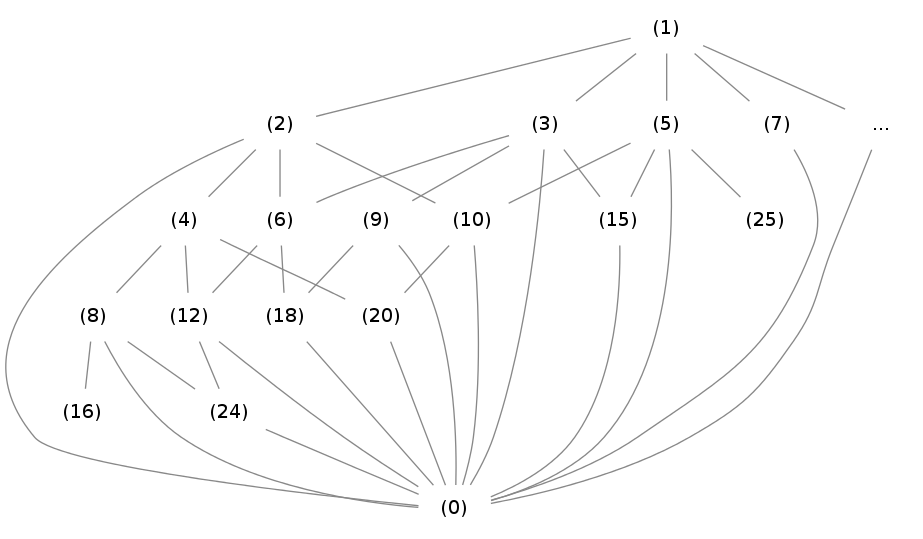
\includegraphics[scale=0.4]{ideale-z}
  \caption{\label{ideale:z}Modulo Platz und klassische Logik eine
  vollständige Übersicht über alle Ideale von~$\ZZ$.}
\end{table}

\begin{aufg}Zeige, dass wenn alle Ideale von~$\ZZ$ von der Form~$(x)$ für
eine ganze Zahl~$x$ sind, das Prinzip vom ausgeschlossenen Dritten gilt.
\emph{Tipp:} Betrachte für eine beliebige Aussage~$\varphi$ das Ideal
$\{ x \in \ZZ \,|\, x = 0 \vee \varphi \} \subseteq \ZZ$ (wieso
sind die Idealaxiome erfüllt?).\end{aufg}


\subsection{Primideale und Nilpotenz}

\begin{defn}Ein Element~$x \in R$ eines Rings~$R$ heißt genau dann
\emph{nilpotent}, wenn eine gewisse Potenz Null ist:
\[ x^n = 0 \qquad\text{für ein~$n \geq 0$}. \]
\end{defn}

\begin{bsp}Im Ring~$\ZZ/(4)$ ist das Element~$[2]$ nilpotent.\end{bsp}

\begin{prop}Die nilpotenten Elemente eines Rings liegen in allen Primidealen
des Rings.\end{prop}
\begin{proof}Sei~$x$ mit~$x^n = 0$ ein nilpotentens Element. Sei~$\pp$ ein
beliebiges Primideal. Dann ist also~$x^n$ in~$\pp$ enthalten. Wegen der
Primalitätsbedingung ist daher auch~$x$ in~$\pp$ enthalten. Das war zu
zeigen.\end{proof}

Interessant ist nun, dass -- in einem klassischen Kontext -- auch die Umkehrung
dieser Proposition gilt. Somit hat man ein einfaches Kriterium an der Hand, um
die Nilpotenz eines Ringelements nachzuweisen.

\begin{prop}[nur klassisch]\label{intersectprim}%
Im Schnitt aller Primideale eines Rings liegen nur
die nilpotenten Elemente.\end{prop}
\begin{proof}Sei~$x$ ein Element von~$R$, welches in allen Primidealen liegt.
Wir wollen zeigen, dass~$x$ nilpotent ist; dazu führen wir einen
Widerspruchsbeweis, nehmen also an, dass~$x$ nicht nilpotent ist. Dann enthält
die Menge
\[ S := \{ x^n \,|\, n \geq 0 \} \subseteq R \]
also nicht die Null. Wir betrachten nun das bezüglich der
Teilmengeninklusionsrelation partiell geordnete Mengensystem
\[ \U := \{ \aa \subseteq R \,|\, \text{$\aa$ ist ein Ideal mit~$\aa \cap S =
\emptyset$} \}. \]
Dieses ist bewohnt: Das Nullideal liegt wegen~$0 \not\in S$ in~$\U$. Außerdem
liegt die Vereinigung~$\bigcup_i \aa_i$ einer in~$\U$ liegenden Kette von
Elementen aus~$\U$ wieder in~$\U$. Damit sind alle Voraussetzung des Lemmas von
Zorn erfüllt, womit~$\U$ also ein maximales Element~$\mm$ enthält.

Man kann nun nachrechnen, dass~$\mm$ ein Primideal ist. Da~$x \not\in \mm$
(wegen~$x \in S$), ist das ein Widerspruch zur Voraussetzung.
\end{proof}

Dieser Beweis ist aus zwei Gründen inhärent klassisch: Zum einen, weil
er ein echter Widerspruchsbeweis ist; zum anderen, weil das Lemma von Zorn
verwendet wird (dieses ist zum Auswahlaxiom äquivalent). Man kann sogar zeigen,
dass ein konstruktiver Beweis dieser Proposition nicht möglich ist. Daher
ist folgendes Meta-Theorem absolut erstaunlich:

\begin{wunder}Sei~$x \in R$ ein Element eines Rings. Sei ein \emph{klassischer
Beweis} (einer gewissen Form) der Aussage~$x \in \pp$, wobei man von~$\pp$ nur
die Axiome eines Primideals voraussetzen darf, gegeben. Dann ist~$x$ nilpotent
(konstruktiv!). Aus dem klassischen Beweis kann man also auf konstruktive Art
und Weise einen konstruktiven Beweis der Nilpotenzbehauptung extrahieren.
\end{wunder}

Die genaue Formulierung steht im Haupttext als Satz~\ref{satz:genprime}.


\subsubsection*{Polynome mit Koeffizienten in Primidealen}

Für das Beispiel in Abschnitt~\ref{bsp:nilpotentepolynome} benötigen wir
folgendes Lemma.
\begin{lemma}\label{produktprim}Seien~$f,g \in R[X]$ Polynome über einem Ring~$R$. Sei~$\pp
\subseteq R$ ein Primideal. Wenn alle Koeffizienten von~$fg$ in~$\pp$ liegen,
so liegen schon alle Koeffizienten von~$f$ oder alle Koeffizienten von~$g$
in~$\pp$.\end{lemma}
Wenn man mit der Faktorringkonstruktion vertraut ist, lässt sich das Lemma
einfacher formulieren: Ist ein Produkt in~$(R/\pp)[X]$ Null, so ist schon einer
der Faktoren in~$(R/\pp)[X]$ Null. Diese Aussage ist Instanz eines noch
allgemeineren Lemmas: Ist ein Ring~$S$ ein Integritätsbereich, so auch~$S[X]$.


\subsection{Radikalideale}

\begin{defn}\label{def:radikal}\begin{enumerate}
\item Ein Ideal~$\aa \subseteq R$ eines Rings~$R$ heißt genau dann
\emph{Radikalideal}, wenn für alle~$x
\in R$ und~$n \geq 0$ aus~$x^n \in \aa$ schon~$x \in \aa$ folgt.
\item Sei~$\aa \subseteq R$ ein Ring. Dann heißt das Ideal
\[ \sqrt{\aa} := \{ x \in R \,|\, \exists n \geq 0{:}\ x^n \in \aa \} \]
das \emph{Radikal von~$\aa$}. Es ist stets ein Radikalideal, und zwar das
kleinste, das~$\aa$ umfasst.
\end{enumerate}\end{defn}

\begin{bsp}Das Ideal~$(12) \subseteq \ZZ$ ist kein Radikalideal, $\sqrt{(12)} =
(6)$ dagegen schon.\end{bsp}

\begin{bem}Die Zuordnung von Radikalen zu Idealen bildet einen
Linksadjungierten zum Vergissfunktor der Kategorie der Radikalideale von~$R$ in
die Kategorie aller Ideale von~$R$.\end{bem}

\begin{lemma}\label{lemma:rad}%
Für die bezüglich der Inklusionsbeziehung partiell geordnete Menge~$\Rad(R)$
der Radikalideale eines Rings~$R$ gilt:
\begin{enumerate}
\item Das kleinste Element ist~$\sqrt{(0)}$, das Ideal aller nilpotenten
Elemente.
\item Das größte Element ist~$(1)$, das Einsideal.
\item Das Supremum zweier Elemente~$\aa,\bb$, also das kleinste Radikalideal,
das~$\aa$ und~$\bb$ umfasst, ist
\[ \sqrt{\aa + \bb} := \{ x \in R \,|\, \text{$x^n = u + v$ für ein~$n \geq 0,
u \in \aa, v \in \bb$} \}. \]
\item Das Infimum zweier Elemente~$\aa,\bb$, also das größte Radikalideal,
das in~$\aa$ und~$\bb$ enthalten ist, ist $\aa \cap \bb$.
\end{enumerate}
\end{lemma}
\begin{proof}Nachrechnen.\end{proof}

\begin{bsp}Für den Ring der ganzen Zahlen gilt~$(6) \cap (5) = (30)$ und~$(6)
\cap (15) = (30)$.\end{bsp}

\begin{bsp}Allgemein gilt
\[ \sup\bigl\{ \sqrt{(x)}, \sqrt{(y)} \bigr\} = \sqrt{\sqrt{(x)} + \sqrt{(y)}} =
\sqrt{(x,y)}. \]
\end{bsp}


\section{Garben}

\label{appendix:garben}

\subsection{Prägarben und Garben}

\begin{defn}\begin{enumerate}
\item Eine \emph{Prägarbe} auf einem topologischen Raum~$X$ (oder einer
Örtlichkeit) ist eine Prägarbe im kategoriellen Sinne auf der
als dünne Kategorie aufgefassten Halb\-ord\-nung~$\Ouv(X)$ der offenen
Teilmengen (bzw.  offenen Dinge) von~$X$, also ein Funktor~$\Ouv(X)^\op \to
\Set$.
\item Ein \emph{Morphismus von Prägarben}~$\F \to \G$ ist eine natürliche
Transformation~$\F \to \G$.
\end{enumerate}
\end{defn}

Ist~$\F$ eine Prägarbe auf~$X$ und~$U \subseteq X$ eine offene
Menge, so schreibt man auch~"`$\Gamma(U, \F)$"' für~$\F(U)$ und nennt die
Elemente dieser Menge \emph{Schnitte von~$\F$ auf~$U$}. Wenn~$V \subseteq U$,
schreibt man die induzierte Abbildung~$F(\text{"`$V \subseteq U$"'}) : \F(U)
\to \F(V)$ auch als~"`$(\freist)|_V$"'. Diese Schreibweise rührt von den
wichtigsten Beispielen für Prägarben her.

Die Prototyp-Beispiele für Prägarben stammen nämlich von verschiedenen
Funktionsbegriffen ab. Etwa gibt es auf jedem topologischen Raum~$X$ die
Prägarbe~$\C^0$ der stetigen Funktionen, definiert über
\[ \begin{array}{@{}rcl@{}}
  \Ouv(X)^\op &\longrightarrow& \Set \\
  U &\longmapsto& \{ U \xra{f} \RR \,|\, \text{$f$ stetig} \} \\
  \text{"`$V \subseteq U$"'} &\longmapsto& \res^U_V
\end{array} \]
mit~$\res^U_V : \C^0(U) \to \C^0(V), f \mapsto f|_V$ der
Einschränkungsabbildung.  Trägt~$X$ sogar die Struktur einer glatten
Mannigfaltigkeit, kann man analog auch die Garbe~$\C^\infty$ der glatten
Funktionen definieren -- man setzt $\Gamma(U, \C^\infty) := \{ U \xra{f} \RR
\,|\, \text{$f$ glatt} \}$.


\subsubsection*{Die Garbenbedingung}

\begin{defn}\begin{enumerate}
\item Eine Prägarbe~$\F$ auf~$X$ heißt genau dann \emph{Garbe}, wenn
folgendes Verklebeaxiom erfüllt ist: Ist~$U = \bigcup_i U_i \subseteq X$ eine
offene Überdeckung einer offenen Teilmenge und ist~$(s_i)_{i \in I}$ eine
Familie von Schnitten mit~$s_i \in \Gamma(U_i, \F)$, welche auf Überlappungen
übereinstimmen, also
$s_i|_{U_i \cap U_j} = s_j|_{U_i \cap U_j}$
für alle Indizes~$i,j$ erfüllen, so soll es genau einen Schnitt~$s \in
\Gamma(U,\F)$ mit~$s|_{U_i} = s_i$ für alle~$i$ geben.
\item Ein \emph{Morphismus von Garben} ist ein Morphismus der zugrundeliegenden
Prägarben.
\end{enumerate}\end{defn}

Die Kategorie der Garben auf~$X$, $\Sh(X)$, ist also eine volle Unterkategorie
der Kategorie der Prägarben auf~$X$, $\PSh(X)$.

\begin{bsp}Die Prägarben~$\C^0$ und~$\C^\infty$ (sofern definierbar) sind
Garben: Man kann stetige bzw. glatte Funktionen, die auf Überlappungen
übereinstimmen, miteinander \emph{verkleben}; die resultierende Funktion wird
wieder stetig bzw. glatt sein.\end{bsp}

\begin{bsp}Die Prägarbe~$\C_{\text{const}}$ der konstanten Funktionen,
\[ \Gamma(U, \C_{\text{const}}) = \{ U \xra{f} \RR \,|\, \text{$f$ konstant}
\}, \]
ist außer in pathologischen Fällen keine Garbe. Denn wenn zwei konstante
Funktionen~$f_1 : U_1 \to \RR$ und~$f_2 : U_2 \to \RR$ auf zwei sich nicht
überlappenden offenen Mengen definiert sind, ist die Kompatibilitätsbedingung
leer, sie lassen sich jedoch im Allgemeinen nicht zu einer konstanten Funktion
auf~$U_1 \cup U_2$ zusammensetzen: Das geht genau dann, wenn sie denselben
konstanten Wert haben. Die analog definierte Prägarbe~$\C_{\text{lc}}$ der
lokal konstanten Funktionen ist dagegen durchaus eine Garbe. (Eine Funktion heißt genau
dann lokal konstant, wenn es eine Überdeckung ihres Urbildbereichs gibt, sodass
die Einschränkungen der Funktion auf die Überdeckungsmengen jeweils konstant
sind.)\end{bsp}

\begin{bem}Es gibt ein allgemeine Technik, die \emph{Garbifizierung}, mit der
man auf universelle Art und Weise aus Prägarben Garben machen kann. (Genauer
ist der Garbifizierungsfunktor linksadjungiert zum Vergissfunktor~$\Sh(X) \to
\PSh(X)$.) Die Garbifizierung der Prägarbe der konstanten Funktionen ist dann
gerade die Garbe der lokal konstanten Funktionen.\end{bem}


\subsubsection*{Globale Schnitte}

Historisch eine der wichtigsten Garben ist die Garbe~$\O_X$ der holomorphen
Funktionen auf einer komplexen Mannigfaltigkeit~$X$ (etwa~$X = \CC$ oder~$X =
\widehat{\CC} = \CC \cup \{ \infty \}$, der riemannschen Zahlenkugel), definiert
über
\[ \Gamma(U, \O_X) = \{ U \xra{f} \CC \,|\, \text{$f$ holomorph} \}. \]
Sie hat die für viele Garben typische Eigenschaft, oftmals nur recht wenige
\emph{globale Schnitte} (Elemente von~$\Gamma(X,\O_X)$) zu besitzen -- im Fall
der riemannschen Zahlenkugel sind das nach dem Satz von Liouville etwa nur
die konstanten Funktionen. Nichttrivial sind nur Schnitte, die auf
kleineren offenen Teilmengen definiert sind.

Sinnvolle Bedingungen an Garben oder Garbenmorphismen erhält man in der Regel
also nur dann, wenn man alle offenen Mengen einbezieht, nicht nur~$X$ selbst.
Die Kripke-Joyal-Semantik zur Interpretation der internen Sprache eines
Garbentopos achtet von selbst darauf (siehe Abschnitt~\ref{internesprache}).


\subsection{Monomorphismen und Epimorphismen von Garben}

\begin{prop}Sei~$\alpha : \F \to \G$ ein Morphismus von Prägarben. Dann gilt:
\begin{enumerate}
\item Der Morphismus~$\alpha$ ist genau dann ein Monomorphismus in~$\PSh(X)$,
wenn für alle offenen Teilmengen~$U \subseteq X$ die Komponente~$\alpha_U :
\Gamma(U,\F) \to \Gamma(U,\G)$ eine injektive Abbildung ist, wenn also gilt:
\[ \forall \text{$U \subseteq X$ offen}\_
  \forall s,t \in \Gamma(U,\F)\_
  \alpha_U(s) = \alpha_U(t) \Rightarrow s = t. \]
\item Der Morphismus~$\alpha$ ist genau dann ein Epimorphismus in~$\PSh(X)$,
wenn für alle offenen Teilmengen~$U \subseteq X$ die Komponente~$\alpha_U :
\Gamma(U,\F) \to \Gamma(U,\G)$ eine surjektive Abbildung ist, wenn also gilt:
\[ \forall \text{$U \subseteq X$ offen}\_
  \forall s \in \Gamma(U,\G)\_
  \exists t \in \Gamma(U,\F)\_
  \alpha_U(t) = s. \]
\end{enumerate}
\end{prop}

\begin{prop}Sei~$\alpha : \F \to \G$ ein Morphismus von Garben. Dann gilt:
\begin{enumerate}
\item Der Morphismus~$\alpha$ ist genau dann ein Monomorphismus in~$\Sh(X)$,
wenn für alle offenen Teilmengen~$U \subseteq X$ die Komponente~$\alpha_U :
\Gamma(U,\F) \to \Gamma(U,\G)$ eine injektive Abbildung ist.
\item Der Morphismus~$\alpha$ ist genau dann ein Epimorphismus in~$\Sh(X)$,
wenn jeder Schnitt von~$\G$ \emph{lokal} ein Urbild besitzt, d.\,h. wenn für
alle offenen Teilmengen~$U \subseteq X$ und Schnitte~$s \in \Gamma(U,\G)$ eine
Überdeckung~$U = \bigcup U_i$ und Schnitte~$t_i \in \Gamma(U_i,\F)$
mit~$\alpha_{U_i}(t_i) = s|_{U_i}$ existieren.
\end{enumerate}
\end{prop}

Wenn man sich das erste Mal mit Garben beschäftigt, verwundert vielleicht die
Charakterisierung von Epimorphismen in der Garbenkategorie: Vielleicht hätte man eher die
Bedingung, dass alle Komponentenabbildungen~$\alpha_U$ surjektiv sind,
erwartet. Diese stärkere Bedingung ist zwar ebenfalls hinreichend für Epimorphie,
aber nur in der größeren Kategorie aller \emph{Prä}garben notwendig.

\begin{bsp}Sei~$\O_X$ die Garbe der holomorphen Funktionen auf~$X = \CC$.
Sei~$\O_X^\times$ die Untergarbe der bezüglich der Multiplikation
invertierbaren holomorphen Funktionen, also der nirgends verschwindenden
Funktionen. Dann ist der "`$\exp$"' genannte Garbenmorphismus
\[ \begin{array}{@{}rrcl@{}}
           & \O_X &\longrightarrow& \O_X^\times \\
  \text{auf $U \subseteq X$:} & f \in \O_X(U) &\longmapsto& \exp \circ f \in
  \O_X^\times(U)
\end{array} \]
ein Epimorphismus (da man \emph{lokal} die Exponentialfunktion mittels eines
geeigneten Zweigs des Logarithmus umkehren kann). Aber seine
Komponentenabbildungen~$\exp_U$ sind nicht alle surjektiv, etwa für solche
Teilmengen~$U$, die einen Kreisring um den Ursprung umfassen.\end{bsp}

\begin{bem}Mit \emph{Garbenkohomologie} kann man \emph{messen}, inwieweit ein
Epimorphismus von Garben davon entfernt ist, auch ein Epimorphismus von
Prägarben zu sein.
\end{bem}

\begin{bem}In den meisten Lehrbüchern sind \emph{Mono-} und \emph{Epimorphismus} speziell
definierte Begriffe: Ein Morphismus~$\alpha : \F \to \G$ von Garben heißt dort genau dann
mono- bzw. epimorph, wenn die induzierten Abbildungen~$\alpha_x : \F_x \to
\G_x$, $x \in X$, auf allen \emph{Halmen} injektiv bzw. surjektiv sind. Diese
Definition ist äquivalent zur allgemeinen kategoriellen Definition und somit
zur Charakterisierung aus der Proposition. Sie hat allerdings den Nachteil, dass sie nicht
unmittelbar auf Örtlichkeiten übertragbar ist.\end{bem}


\nocite{*}
\printbibliography

\end{document}


\section{Elemente in Kategorien}

\subsection{Globale und verallgemeinerte Elemente}

Sei~$X \xra{f} Y$ eine Abbildung von Mengen. Bekanntlich heißt diese genau dann
\emph{injektiv}, wenn
\begin{equation}\label{inj}
  \forall x,x' \in X\_\ f(x) = f(x') \ \Longrightarrow\  x = x'.
\end{equation}
Diese Bedingung lässt sich nicht nur in~$\Set$, sondern in jeder Kategorie
interpretieren, deren Objekte Mengen mit Zusatzstruktur und deren Morphismen
gewisse Abbildungen sind. Wenn man aber über solche Kategorien hinaus
verallgemeinern möchte, muss man die Aussage in kategorieller Notation
umschreiben; sie lautet dann:
\begin{equation}\label{injcat}
  \forall (1 \xra{x} X), (1 \xra{x'\!} X)\_\ f \circ x = f \circ x'
  \ \Longrightarrow\  x = x'.
\end{equation}
Morphismen der Form~$1 \to X$ heißen \emph{globale Elemente} von~$X$.
Bedingung~\eqref{injcat} lässt sich in allen Kategorien interpretieren, in denen es ein
terminales Objekt~$1$ gibt, und ist in~$\Set$ äquivalent zur mengensprachlich
formulierten Bedingung~\eqref{inj}. Das hat einen tieferen Grund: In~$\Set$ ist
die einelementige Menge~$1 = \{ \star \}$ ein \emph{Erzeuger}, d.\,h. Objekte
in~$\Set$ sind schon durch ihre globalen Elemente (bis auf Isomorphie) eindeutig bestimmt.

In Kategorien, in denen das terminale Objekt aber kein Erzeuger ist, ist
Bedingung~\eqref{injcat} dagegen nicht sehr aussagekräftig. Konkret der Fall
ist das beispielsweise beim Topos~$\Sh(A)$ der Garben auf einem topologischen
Raum~$A$. Globale Elemente einer Garbe~$\F$ stehen in natürlicher Bijektion mit
globalen Schnitten~$x \in \F(A)$ (daher der Name), sodass
Bedingung~\eqref{injcat} nur aussagt, dass die Garbenabbildung~$f$
\emph{injektiv auf globalen Schnitten} ist. Da viele interessante Garben
überhaupt keine oder nur wenige globale Schnitte besitzen, ist das in der Regel
eine gehaltlose Aussage.

Man löst das Problem dadurch, indem man nicht nur globale Elemente~$1 \to X$,
sondern auch \emph{verallgemeinerte} Elemente~$I \to X$ betrachtet. Dabei
muss~$I$ alle Objekte der untersuchten Kategorie~$\C$ durchlaufen; mit diesem
Prinzip ist eine bessere Übersetzung der Injektivitätsbedingung die Aussage
\begin{equation}\label{injallg}
  \forall \text{Objekte $I$ in~$\C$}\_ \forall (I \xra{x} X), (I \xra{x'\!} X) \text{ in~$\C$}\_\ 
  f \circ x = f \circ x' \ \Longrightarrow\ x = x',
\end{equation}
und diese fängt die Intuition hinter dem Injektivitätsbegriff auch in
beliebigen Kategorien~$\C$ richtig ein: Ein Morphismus~$f$, der
Bedingung~\eqref{injallg} erfüllt, heißt bekanntlich \emph{Monomorphismus}. Den
tieferen Grund, wieso diese Idee funktioniert, drückt das
\emph{Yonedalemma}~\cite{yoneda} aus, demnach ein Objekt (bis auf Isomorphie) schon
eindeutig durch die Morphismen in das Objekt hinein bestimmt ist.
% XXX: Letzten Satz verstehe ich nicht?


\subsection{Die interne Sprache}

In der Praxis ist es allerdings umständlich, immer an verallgemeinerte
Elemente denken und diese in der Notation berücksichtigen zu müssen. Als
Abhilfe dazu gibt es die \emph{interne Sprache} einer Kategorie
(nach J.~Bénabou, A.~Joyal und W.~Mitchell, siehe~\cite[Kap.~1]{catlogprime}):
In dieser
kann man die Injektivitätsbedingung als
\begin{equation}\label{injtype}
  \forall x,x'\?X\_\ f(x) = f(x') \ \Longrightarrow\ x = x'
\end{equation}
formulieren, die Ähnlichkeit zur ursprünglichen Definition~\eqref{inj} ist
offensichtlich. Der Doppelpunkt beim Allquantor soll andeuten, dass~$X$ nicht
notwendigerweise eine Menge und~$x,x'$ nicht notwendigerweise Elemente einer
Menge im wörtlichen (materiellen) Sinn sein müssen. Stattdessen sagt man,
dass~$X$ ein \emph{Typ} und~$x,x'$ \emph{Werte} dieses Typs sind, und
bezeichnet den Ausdruck~\eqref{injtype} als \emph{Aussage im leeren Kontext}.
(Freie, nicht durch Quantoren gebundene Variablen sammelt der sog. Kontext
der Aussage auf.)

Wenn die untersuchte Kategorie genügend gute Eigenschaften hat -- ein
\emph{Topos} ist --, gibt es ein konkretes, algorithmisch gegebenes und auch in der Praxis einfach
durch\-führ\-ba\-res Verfahren, um solche intern formulierten Aussagen in die externe
mathematische Sprache zu übersetzen, die sog.
\emph{Kripke-Joyal-Semantik}~\cite[Kap~VI.6]{moerdijkmaclane}.
Wendet man dieses auf die Aussage~\eqref{injtype} an, erhält man (nach einem
Vereinfachungsschritt) genau die zuvor hergeleitete Bedingung~\eqref{injallg}
mit verallgemeinerten Elementen.

Die interne Sprache erlaubt nicht nur, Bedingungen einfach formulieren zu
können, sondern auch logische Schlussfolgerungen anzustellen. Beispielsweise
kann man, indem man den üblichen Beweis mit
minimalen syntaktischen Änderungen abschreibt, intern zeigen, dass
\[ \speak{$f$ ist injektiv} \wedge \speak{$f$ ist surjektiv}
  \Longrightarrow \speak{$f$ besitzt eine Umkehrfunktion}. \]
Die Häkchen sollen andeuten, dass die Teilaussagen nur umgangssprachlich vorliegen und
daher vom Leser formalisiert werden müssen.
Extern besagt diese Implikation, dass jeder Morphismus~$f$ eines Topos, der zugleich ein
Mono- und Epimorphismus ist, schon einen Umkehrmorphismus besitzt, also ein
Isomorphismus ist.


\subsection{Beschränkung auf intuitionistische Logik}

Damit die Übersetzungen intern bewiesener Schlussfolgerungen
in beliebigen Topoi gültig sind, ist man beim Beweisen aber einer Reihe von
Einschränkungen unterworfen: Man darf in Abgrenzung der gewohnten klassischen
Logik nur die Schlussregeln
\emph{intuitionistischer Logik}~\cite{dalen} verwenden, d.\,h. man muss auf das Prinzip vom
ausgeschlossenen Dritten, demnach man für jede Aussage~$\phi$ voraussetzen
darf, dass
\[ \phi \vee \neg\phi \]
gilt, verzichten; und ebenso kann man das Prinzip der
Doppelnegationselimination ("`$\neg\neg\phi \Rightarrow \phi$"') und das
Auswahlaxiom nicht verwenden. Infolgedessen sind Widerspruchsbeweise
("`um~$\phi$ zu zeigen, zeige, dass~$\neg\phi$ falsch ist"') nicht
zulässig.\footnote{Davon unbetroffen sind Beweise negierter Aussagen, d.\,h.
Aussagen der Form~$\neg\psi$. Das übliche Vorgehen ("`Gelte $\psi$. Dann
\ldots, also Widerspruch."') ist für solche zulässig, es handelt sich dabei
nicht um Widerspruchsbeweise im eigentlichen Sinn. Klassisch kann man den
Unterschied nicht erkennen, da man gewohnt ist, nach Belieben doppelte
Verneinungen einzuführen oder zu streichen.} Zwei Beispiele sollen dieses
Phänomen am Garbentopos~$\Sh(A)$ über einem topologischen Raum~$A$ verdeutlichen:
\begin{enumerate}
\item Dass eine Aussage~$\phi$ der internen Sprache von~$\Sh(A)$ gilt, kann man
sich so vorstellen, dass sie auf jeder offenen Teilmenge~$U \subseteq A$
erfüllt ist. Die doppelte Negation~$\neg\neg\phi$ bedeutet dagegen nur, dass
jede nichtleere offene Teilmenge~$U \subseteq A$ eine weitere, kleinere nichtleere offene
Teilmenge~$V \subseteq U$ enthält, auf der~$\phi$ gilt.

Sei etwa~$A = \RR$ die reelle Zahlengerade und~$f$ eine stetige reellwertige Funktion
auf~$\RR$. Dann bedeutet die interne Aussage
\[ \speak{$f$ ist (bzgl. der Multiplikation) invertierbar}, \]
dass~$f$ auf jeder offenen Teilmenge
invertierbar ist, also dass~$f(a) \neq 0$ für alle~$a \in A$. Die doppelt
negierte Aussage dagegen wird beispielsweise auch von Funktionen erfüllt, die
isolierte Nullstellen besitzen, und allgemeiner von allen Funktionen, die auf
keinem Intervall konstant null sind.
% XXX: Also auf einer dichten Menge nicht null sind!

\item Sei~$A = \CC$ die komplexe Zahlenebene und~$f$ eine auf ganz~$\CC$
definierte holomorphe Funktion. Holomorphe Lösungen der Funktionalgleichung
\[ \exp(g) = f \]
organisieren sich auf natürliche Art und Weise in einer Garbe~$\F$ auf~$\CC$,
explizit durch die Setzung
\begin{equation}\label{holsheaf}
  \F(U) = \{ U \xra{g} \CC \,|\, \text{$g$ holomorph und~$\exp(g) = f$ auf~$U$} \}
\end{equation}
für offene Teilmengen~$U \subseteq \CC$ gegeben. Wenn~$f$ Nullstellen besitzt,
ist die Aussage $\exists g\?\F$ der internen Sprache nicht erfüllt: Diese
bedeutet nämlich, dass es eine Überdeckung von~$\CC$ durch offene Mengen gibt,
sodass es auf jeder dieser offenen Mengen~$U$ jeweils eine auf~$U$ definierte Lösung
der Funktionalgleichung gibt (wobei diese Teillösungen auf Überlappungen nicht
unbedingt zusammenpassen müssen) -- das kann man kurz als das Motto \emph{Existenz in der
internen Sprache bedeutet lokale Existenz} ausdrücken. Aber in jeder solchen Überdeckung würde
mindestens eine offene Menge~$U$ eine Nullstelle von~$f$ enthalten, und auf
einer solchen Menge ist die Funktionalgleichung natürlich nicht erfüllbar.

Es gilt aber die doppelt negierte Aussage~$\neg\neg(\exists g\?\F)$, denn zu
jeder nichtleeren offenen Teilmenge~$U \subseteq \CC$ kann man eine genügend
kleine weitere nichtleere offene Teilmenge~$V \subseteq U$ finden, die keine
Nullstellen von~$f$ enthält (diese sind ja isoliert) und auf der es einen
passenden Logarithmus gibt.
\end{enumerate}

% XXX: \seq{} erzeugt falschen horizontalen Freiraum.

% Mögliche weitere Themen:
% * Lindenbaumzeugs
% * Suche auf unendlichen Datentypen
% * Andrejs Gems and Stones
% * Arbeit mit universellen Objekten und Elementen
%   (vielleicht erstmal universelle Ringelemente,
%   dann universelle Objektelemente (Scheibentopoi)
%   und zuletzt universelle Objekte (E[X]))
% * Mutter aller Monaden verstehen. Was ist die logische Interpretation?

% Im nächsten Vortrag erklären:
% * konkrete vs. abstrakte Aussagen
% * Hilberts Programm
% * verschiedene Stufen für Schlimmheit von LEM
% * "Von konkreten Aussagen sollte es konkrete Beweise geben"
% * Proof mining auch für Beweise aus der Analysis relevant,
%   siehe etwa Kohlenbach, Applied Proof Theory.
% * Grund, wieso PA/HA inkonsistent sein KÖNNTE
% * Gelfand-Schneider-FUD wieder auflösen
%
% Dazu noch herausfinden:
% * historischer Umgang mit LEM
% * Theorem von Barr verstehen. Ist es wirklich nicht konstruktiv?
%   Bezug zu Friedmans Trick?
%
% Ideen für Übungsaufgaben:
% * Bei Coquand und Troelstra inspirieren lassen.

% Literatur:
% * http://math.stanford.edu/~feferman/papers/highlights.pdf

% Steve Russ. The Mathematical Works of Bernard Bolzano.
% Google Docs Seite 276 und vorher.
% http://books.google.de/books?id=zp7cLQn0x3gC&lpg=PA146&ots=riM_BDSt8G&dq=bolzano%20early%20analysis%20rb&hl=de&pg=PA276#v=onepage&q&f=false

% Weglassen von Variablen geht nicht (und folgt auch nicht aus struktureller
% Regel)
% Logik-Geist
% Mutter aller Monaden

% Diagramm zur internen Algebra
% Geister-Abbildung
% Cover

% Bornsche Regel

% Jordan-Algebra
% Bohr-Topos als *Garben*topos
% Quantornotation einheitlich machen

% verschiedene Schulen

% C(Kompaktifizierung)

% Das Beispiel RH ==> Beh, neg-RH ==> Beh.

% Ausblick: Gödel richtig verstehen:
% Lambek, Reflections on a categorical foundations of mathematics

% Artemov.pdf

% Intuitionismus vs. russischer Konstruktivismus;
% siehe http://staff.science.uva.nl/~ulle/teaching/lolaco/2013/slides/vdberg.pdf.
% Das auch als Quelle aufnehmen!

% Beispiel-Topos: Klassifizierender Topos zur Theorie der Gruppen oder so

% Problem mit der BHK-Interpretation nennen

% http://video.ias.edu/members/1213/0318-AndrejBauer

% XXX: Stetigkeitsnachweise unnötig

% "demnach"

% können wir Corfield zitieren?

% Sind alle Quellen zitiert? Nein, coquand:classical zum Beispiel nicht.

In einer hyphotetischen überarbeiteteten Version:

- Inwieweit genau ist konstruktive Logik philosophisch einfacher zu
  rechtfertigen als klassische?

- Kann man konstruktive Logik sinnvoll in Philosophie selbst anwenden?

- Ausführen: Curry-Howard im Kontext formaler Methoden
